%%%%%%%%%%%%%%%%%%%%%%%%%%%%%%%%%%%%%%%%%
% Masters/Doctoral Thesis 
% LaTeX Template
% Version 2.5 (27/8/17)
%
% This template was downloaded from:
% http://www.LaTeXTemplates.com
%
% Version 2.x major modifications by:
% Vel (vel@latextemplates.com)
%
% This template is based on a template by:
% Steve Gunn (http://users.ecs.soton.ac.uk/srg/softwaretools/document/templates/)
% Sunil Patel (http://www.sunilpatel.co.uk/thesis-template/)
%
% Template license:
% CC BY-NC-SA 3.0 (http://creativecommons.org/licenses/by-nc-sa/3.0/)
%
%%%%%%%%%%%%%%%%%%%%%%%%%%%%%%%%%%%%%%%%%

%----------------------------------------------------------------------------------------
%	PACKAGES AND OTHER DOCUMENT CONFIGURATIONS
%----------------------------------------------------------------------------------------

\documentclass[
11pt, % The default document font size, options: 10pt, 11pt, 12pt
%oneside, % Two side (alternating margins) for binding by default, uncomment to switch to one side
english, % ngerman for German
singlespacing, % Single line spacing, alternatives: onehalfspacing or doublespacing
%draft, % Uncomment to enable draft mode (no pictures, no links, overfull hboxes indicated)
%nolistspacing, % If the document is onehalfspacing or doublespacing, uncomment this to set spacing in lists to single
%liststotoc, % Uncomment to add the list of figures/tables/etc to the table of contents
%toctotoc, % Uncomment to add the main table of contents to the table of contents
%parskip, % Uncomment to add space between paragraphs
%nohyperref, % Uncomment to not load the hyperref package
headsepline, % Uncomment to get a line under the header
%chapterinoneline, % Uncomment to place the chapter title next to the number on one line
%consistentlayout, % Uncomment to change the layout of the declaration, abstract and acknowledgements pages to match the default layout
]{MastersDoctoralThesis} % The class file specifying the document structure

\usepackage[utf8]{inputenc} % Required for inputting international characters
\usepackage[T1]{fontenc} % Output font encoding for international characters
\usepackage{mathpazo} % Use the Palatino font by default

%\usepackage[backend=bibtex,style=numeric,natbib=true,sorting=none]{biblatex} % Use the bibtex backend with the authoryear citation style (which resembles APA)
\usepackage{cite}
\bibliographystyle{atlasBibStyleWithTitle}
%\addbibresource{main.bib} % The filename of the bibliography
\usepackage[autostyle=true]{csquotes} % Required to generate language-dependent quotes in the bibliography
\usepackage{amssymb}  % to have some symbol I don't remember
\usepackage{multirow}
\usepackage{times} % to have tilde
\usepackage{textcomp} % to have tilde
\usepackage{amsmath} % to have math symbols, e.g. binom
\usepackage{mathtools}
\usepackage{slashed} % to have slashed
\usepackage{subfigure}
\usepackage{enumitem} % to personalize enumerations
\usepackage{lscape} % to have tables in landscape mode
\usepackage{pifont}% http://ctan.org/pkg/pifont       
\usepackage{mainstyle}                                                                                
\usepackage{afterpage}
\usepackage{placeins} % \FloatBarrier
%\usepackage[nonumberlist,nopostdot,toc,acronym,nogroupskip]{glossaries} % to make a glossary
\usepackage[colorlinks=false,linkcolor=black]{hyperref}
\usepackage{glossaries} % to make a glossary

\makeglossaries

\newacronym{atlas}{ATLAS}{A Toroidal LHC Apparatus}
\newacronym{bdt}{BDT}{Boosted Decision Tree}
\newacronym{bib}{BIB}{Beam-Induced Background}
\newacronym{cjvf}{corrJVF}{Jet Vertex Fraction}
\newacronym{ecal}{ECal}{Electromagnetic Calorimeter}
\newacronym{eb}{EB}{Extended Barrel}
\newacronym{em}{EM}{Electromagnetic}
\newacronym{gsc}{GSC}{Global Sequential Calibration}
\newacronym{hcal}{HCal}{Hadronic Calorimeter}
\newacronym{ibl}{IBL}{Insertable B-Layer}
\newacronym{id}{ID}{Inner Detector}
\newacronym{jer}{JER}{Jet Energy Resolution}
\newacronym{jes}{JES}{Jet Energy Scale}
\newacronym{jvf}{JVF}{Jet Vertex Fraction}
\newacronym{jvt}{JVT}{Jet Vertex Tagger}
\newacronym{lb}{LB}{Long Barrel}
\newacronym{lar}{LAr}{Liquid Argon}
\newacronym{llr}{LLR}{Log-Likelihood Ratio}
\newacronym{lub}{LB}{Luminosity Barrel}
\newacronym{lhc}{LHC}{Large Hadron Collider}
\newacronym{mc}{MC}{Monte Carlo}
\newacronym{mdt}{MDT}{Monitored Drift Tubes}
\newacronym{ms}{MS}{Muon Spectrometer}
\newacronym{ncb}{NCB}{Non-Collisional Background}
\newacronym{np}{NP}{Nuisance Parameters}
\newacronym{op}{OP}{Operating Point}
\newacronym{pmt}{PMT}{Photon Multiplier Tube}
\newacronym{pdf}{PDF}{Probability Density Function}
\newacronym{partdf}{PDF}{Parton Distribution Function}
\newacronym{pp}{$p-p$}{proton-proton}
\newacronym{pv}{PV}{Primary Vertex}
\newacronym{sct}{SCT}{Semiconductor Tracker}
\newacronym{sm}{SM}{Standard Model}
\newacronym{susy}{SUSY}{Supersymmetry}
\newacronym{trd}{TRD}{Transition Radiation Detector}
\newacronym{trt}{TRT}{Transition Radiation Tracker}


%----------------------------------------------------------------------------------------
%	MARGIN SETTINGS
%----------------------------------------------------------------------------------------

\geometry{
	paper=a4paper, % Change to letterpaper for US letter
	%inner=2.5cm, % Inner margin original
	%outer=3.8cm, % Outer margin original
	inner=1.9cm, % mio!
	outer=2.5cm, % mio!
	bindingoffset=.5cm, % Binding offset
	top=1.5cm, % Top margin
	bottom=1.5cm, % Bottom margin
	%showframe, % Uncomment to show how the type block is set on the page
}

% indentation
\setlength\parindent{15pt}
%\linespread{1.15}

%----------------------------------------------------------------------------------------
%	THESIS INFORMATION
%----------------------------------------------------------------------------------------

\thesistitle{Searches for supersymmetric particles in final states with multiple top and bottom quarks with the ATLAS detector} % Your thesis title, this is used in the title and abstract, print it elsewhere with \ttitle
\supervisor{Dr. Aurelio \textsc{Juste}} % Your supervisor's name, this is used in the title page, print it elsewhere with \supname
\examiner{} % Your examiner's name, this is not currently used anywhere in the template, print it elsewhere with \examname
\degree{Doctor of Philosophy} % Your degree name, this is used in the title page and abstract, print it elsewhere with \degreename
\author{Chiara \textsc{Rizzi}} % Your name, this is used in the title page and abstract, print it elsewhere with \authorname
\addresses{} % Your address, this is not currently used anywhere in the template, print it elsewhere with \addressname

\subject{Physics} % Your subject area, this is not currently used anywhere in the template, print it elsewhere with \subjectname
\keywords{} % Keywords for your thesis, this is not currently used anywhere in the template, print it elsewhere with \keywordnames
\university{\href{http://www.university.com}{UAB}} % Your university's name and URL, this is used in the title page and abstract, print it elsewhere with \univname
\department{\href{http://department.university.com}{Department of Physics}} % Your department's name and URL, this is used in the title page and abstract, print it elsewhere with \deptname
\group{\href{http://researchgroup.university.com}{IFAE}} % Your research group's name and URL, this is used in the title page, print it elsewhere with \groupname
\faculty{\href{http://faculty.university.com}{Faculty of Science}} % Your faculty's name and URL, this is used in the title page and abstract, print it elsewhere with \facname

\AtBeginDocument{
\hypersetup{pdftitle=\ttitle} % Set the PDF's title to your title
\hypersetup{pdfauthor=\authorname} % Set the PDF's author to your name
\hypersetup{pdfkeywords=\keywordnames} % Set the PDF's keywords to your keywords
}

\usepackage{titlesec, blindtext, xcolor}
\newcommand{\hsp}{\hspace{20pt}}
\titleformat{\chapter}[hang]
    {\Huge\bfseries} {\textcolor{red} \thechapter \hsp \textcolor{gray} {|} \hsp} {0pt} {\Huge\bfseries}

%\titleformat{\section}[hang]
%    {\Large\bfseries} {\textcolor{red} \thesection \hsp \textcolor{gray} {|} \hsp} {0pt} {\Large\bfseries}



\begin{document}

\frontmatter % Use roman page numbering style (i, ii, iii, iv...) for the pre-content pages

\pagestyle{plain} % Default to the plain heading style until the thesis style is called for the body content

%----------------------------------------------------------------------------------------
%	TITLE PAGE
%----------------------------------------------------------------------------------------

\begin{titlepage}
\begin{center}

% logos %%%%%%%%%%%%%%%%%%%%%%%%%%%%%%%%%%%%%%%%%%%%
\begin{figure}[h!]
\includegraphics[height=15mm]{figures/front/IFAE_logo}
\hfill
\includegraphics[height=15mm]{figures/front/uab_logo}
\end{figure}
 
% title %%%%%%%%%%%%%%%%%%%%%%%%%%%%%%%%%%%%%%%%%%%%
\vspace{0.5cm}
\HRule\\
\vspace{0.2cm}
{\huge \bf Searches for supersymmetric particles in final states with multiple top and bottom quarks with the ATLAS detector\\
\vspace{1cm}
Ph.D. dissertation}
\HRule\\
\par
\vspace{1.5in}
 
% author %%%%%%%%%%%%%%%%%%%%%%%%%%%%%%%%%%%%%%%%%%%
{\LARGE \bf Chiara Rizzi}
\vspace{0.3cm}
\par
Institut de F\'{i}sica d'Altes Energies\\
Universitat Aut\`{o}noma de Barcelona\\
Departament de F\'{i}sica\\
Facultat de Ci\`{e}ncies \\
Edifici Cn E-08193 Bellaterra (Barcelona)
\par
\vspace{0.5in}
 
 
% supervisor %%%%%%%%%%%%%%%%%%%%%%%%%%%%%%%%%%%%%%
\vfill
{\it Thesis director}\\
Aurelio Juste Rozas\\
ICREA / Institut de F\'{i}sica d'Altes Energies\\
Universitat Aut\`{o}noma de Barcelona\\
Edifici Cn E-08193 Bellaterra (Barcelona)

% tutor %%%%%%%%%%%%%%%%%%%%%%%%%%%%%%%%%%%%%%
\vfill
{\it Thesis tutor}\\
Maria Pilar Casado Lechuga\\
Universitat Aut\`{o}noma de Barcelona / Institut de F\'{i}sica d'Altes Energies\\
Universitat Aut\`{o}noma de Barcelona\\
Edifici Cn E-08193 Bellaterra (Barcelona)

\end{center}
\end{titlepage}

\sloppy
\titlepage
\cleardoublepage

%----------------------------------------------------------------------------------------
%	QUOTATION PAGE
%----------------------------------------------------------------------------------------

%\vspace*{0.2\textheight}
%\noindent\enquote{\itshape Thanks to my solid academic training, today I can write hundreds of words on virtually any topic without possessing a shred of information, which is how I got a good job in journalism.}\bigbreak
%\hfill Dave Barry

%----------------------------------------------------------------------------------------
%	ABSTRACT PAGE
%----------------------------------------------------------------------------------------

%\begin{abstract}
%\addchaptertocentry{\abstractname} % Add the abstract to the table of contents
%\chapter*{Abstract}

This dissertation presents two searches for Supersymmetry in proton-proton collisions at CERN's Large Hadron Collider (LHC), 
targeting signal models that lead to the production of multiple top quarks or bottom quarks in the final state.

The first search targets gluino pair production, where each gluino decays through a top squark (Gtt model) or a bottom squark (Gbb model) 
to a top-antitop quark pair or a bottom-antibottom quark pair, respectively, and a neutralino, which is the Lightest Sypersymmetric Partner (LSP).
Each top quark in turn decays to a $W$ boson and an a bottom quark.
Thus, the final state is characterized by a high multiplicity of bottom jets, which are collimated sprays of particles originating from the hadronization of bottom quarks, and 
missing transverse momentum (\met) from the LSP that escapes the detection. 

The second search targets a GGM model of higgsino pair production, 
where each higgsino decays to a Standard Model Higgs boson and 
a gravitino, which in this case plays the role of the LSP. 
This search focuses on the decay of the two Higgs bosons to bottom-antibottom quark pairs, yielding again final states with multiple $b$-jets.
This is the first ATLAS analysis targeting this signature, which had been 
previously considered in searches performed by the CMS Collaboration.

Both searches in the thesis use the data collected by the ATLAS experiment at the LHC 
between 2015 and 2016, at a center-of-mass energy  \cmtre TeV,
corresponding to an integrated luminosity of 36.1 \ifb.
The gluino search, without further reoptimization, is also extended using the data collected in 2017, for a total integrated luminosity of 79.8 \ifb.

No significant excess of events above the Standard Model expectation is observed in any of the search regions, 
and the results are used to set upper limits on the production of supersymmetric particles. 
The first search excludes at 95\% confidence level gluino masses up to 2.25 TeV for the Gtt model 
and up to 2.17 TeV for the Gbb model, in both cases for neutralino masses below 800 GeV.
The second search excludes higgsino masses in the range 240--880 GeV, assuming 
that the higgsino decays exclusively to a Higgs boson and a gravitino. 

\par\bigskip
\par\bigskip 
\par\bigskip

\noindent \textbf{Keywords}: particle physics, CERN, LHC, ATLAS, supersymmetry, new phenomena, search, top quark, Higgs boson. 

%\end{abstract}

\chapter*{Abstract}

This dissertation presents two searches for Supersymmetry in proton-proton collisions at CERN's Large Hadron Collider (LHC), 
targeting signal models that lead to the production of multiple top quarks or bottom quarks in the final state.

The first search targets gluino pair production, where each gluino decays through a top squark (Gtt model) or a bottom squark (Gbb model) 
to a top-antitop quark pair or a bottom-antibottom quark pair, respectively, and a neutralino, which is the Lightest Sypersymmetric Partner (LSP).
Each top quark in turn decays to a $W$ boson and an a bottom quark.
Thus, the final state is characterized by a high multiplicity of bottom jets, which are collimated sprays of particles originating from the hadronization of bottom quarks, and 
missing transverse momentum (\met) from the LSP that escapes the detection. 

The second search targets a GGM model of higgsino pair production, 
where each higgsino decays to a Standard Model Higgs boson and 
a gravitino, which in this case plays the role of the LSP. 
This search focuses on the decay of the two Higgs bosons to bottom-antibottom quark pairs, yielding again final states with multiple $b$-jets.
This is the first ATLAS analysis targeting this signature, which had been 
previously considered in searches performed by the CMS Collaboration.

Both searches in the thesis use the data collected by the ATLAS experiment at the LHC 
between 2015 and 2016, at a center-of-mass energy  \cmtre TeV,
corresponding to an integrated luminosity of 36.1 \ifb.
The gluino search, without further reoptimization, is also extended using the data collected in 2017, for a total integrated luminosity of 79.8 \ifb.

No significant excess of events above the Standard Model expectation is observed in any of the search regions, 
and the results are used to set upper limits on the production of supersymmetric particles. 
The first search excludes at 95\% confidence level gluino masses up to 2.25 TeV for the Gtt model 
and up to 2.17 TeV for the Gbb model, in both cases for neutralino masses below 800 GeV.
The second search excludes higgsino masses in the range 240--880 GeV, assuming 
that the higgsino decays exclusively to a Higgs boson and a gravitino. 

\par\bigskip
\par\bigskip 
\par\bigskip

\noindent \textbf{Keywords}: particle physics, CERN, LHC, ATLAS, supersymmetry, new phenomena, search, top quark, Higgs boson. 

\chapter*{Resumen}

En esta tesis se presentan dos b\'usquedas de Supersimetr\'ia en colisiones prot\'on-prot\'on en el Gran Colisionador de Hadrones (LHC, por sus siglas en ingl\'es) del CERN,
centradas en modelos que dan lugar a la producci\'on de m\'ultiples quarks top o quarks bottom en el estado final.

La primera b\'usqueda tiene como objetivo la producci\'on de pares de gluinos, donde cada gluino de desintegra a trav\'es de un squark top (modelo Gtt) o un squark  
bottom (modelo Gbb) en una pareja de quarks top-antitop o bottom-antibottom, respectivamente, y un neutralino, que es la part\'icula supersim\'etrica m\'as ligera 
(LSP, por sus siglas en ingl\'es). Cada quak top a su vez se desintegra en un bos\'on $W$ y un quark bottom.
Consecuentemente, el estado final se caracteriza por una alta multiplicidad de bottom jets ($b$-jets), que son chorros de part\'iculas resultantes de
la hadronizaci\'on de quarks bottom, as\'i como un alto momento transverso faltante (\met) debido a que la LSP escapa sin ser detectada. 

La segunda b\'usqueda tiene como objetivo la producci\'on de pares de Higgsinos en el contexto de un modelo GGM, en el cual cada Higgsino 
se desintegra en el bos\'on de Higgs del Model Est\'andar y un gravitino, que en este caso juega el papel de la LSP.
Esta b\'usqueda se centra en sucesos donde ambos bosones de Higgs se desintegran en parejas de quarks bottom-antibottom, de nuevo dado lugar a estados finales 
con m\'ultiples $b$-jets. 
Este es el primer an\'alisis en ATLAS optimizado para esta signatura, la cual hab\'ia sido considerada previamente en b\'usquedas llevadas a cabo por
la colaboraci\'on CMS.

Ambas b\'usquedas en esta tesis usan los datos recopilados por el experimento ATLAS en el LHC 
entre el 2015 y el 2016, a una energ\'ia del centro de masas de \cmtre TeV,
correspondiente a una luminosidad integrada de 36.1 \ifb.
La b\'usqueda de gluinos, sin optimizaci\'on adicional, ha sido extendida usando los datos recopilados en el 2017, resultando en una luminosidad integrada total de 79.8 \ifb.

No habiendo encontrado un exceso significativo de sucesos sobre la predicci\'on del Modelo Est\'andar en ninguna de las regiones de b\'usqueda,
los resultados han sido usados para establecer l\'imites superiores a la producci\'on de part\'iculas supersim\'etricas.
La primera b\'usqueda excluye a un nivel de confianza del 95\% masas del gluino de hasta 2.25 TeV para el modelo Gtt
y de hasta 2.17 TeV para el modelo Gbb, en ambos casos para masas del neutralino menores que 800 GeV.
La segunda b\'usqueda excluye masas del Higgsino en el rango de 240--880 GeV, asumiendo que 
el Higgsino se desintegra exclusivamente en un bos\'on de Higgs y un gravitino.

\par\bigskip
\par\bigskip 
\par\bigskip

\noindent \textbf{Palabras clave}: f\'isica de part\'iculas, CERN, LHC, ATLAS, supersimetr\'ia, nuevos fen\'omenos, b\'usqueda, quark top, bos\'on de Higgs.




%----------------------------------------------------------------------------------------
%	LIST OF CONTENTS/FIGURES/TABLES PAGES
%----------------------------------------------------------------------------------------

\tableofcontents % Prints the main table of contents

%----------------------------------------------------------------------------------------
%	ABBREVIATIONS
%----------------------------------------------------------------------------------------

%\begin{abbreviations}{ll} % Include a list of abbreviations (a table of two columns)
%\textbf{LAH} & \textbf{L}ist \textbf{A}bbreviations \textbf{H}ere\\
%\textbf{WSF} & \textbf{W}hat (it) \textbf{S}tands \textbf{F}or\\
%\end{abbreviations}

%----------------------------------------------------------------------------------------
%	PHYSICAL CONSTANTS/OTHER DEFINITIONS
%----------------------------------------------------------------------------------------

%\begin{constants}{lr@{${}={}$}l} % The list of physical constants is a three column table
% The \SI{}{} command is provided by the siunitx package, see its documentation for instructions on how to use it
%Speed of Light & $c_{0}$ & \SI{2.99792458e8}{\meter\per\second} (exact)\\
%Constant Name & $Symbol$ & $Constant Value$ with units\\
%\end{constants}

%----------------------------------------------------------------------------------------
%	SYMBOLS
%----------------------------------------------------------------------------------------

%\begin{symbols}{lll} % Include a list of Symbols (a three column table)
%$a$ & distance & \si{\meter} \\
%$P$ & power & \si{\watt} (\si{\joule\per\second}) \\
%Symbol & Name & Unit \\
%\addlinespace % Gap to separate the Roman symbols from the Greek
%$\omega$ & angular frequency & \si{\radian} \\
%\end{symbols}

%----------------------------------------------------------------------------------------
%	DEDICATION
%----------------------------------------------------------------------------------------
%\dedicatory{For/Dedicated to/To my\ldots} 
%----------------------------------------------------------------------------------------
%	THESIS CONTENT - CHAPTERS
%----------------------------------------------------------------------------------------

\mainmatter % Begin numeric (1,2,3...) page numbering

\pagestyle{thesis} % Return the page headers back to the "thesis" style

% Include the chapters of the thesis as separate files from the Chapters folder
% Uncomment the lines as you write the chapters

\renewcommand{\arraystretch}{1.6}

%\section{Bib}
%\cite{ATLAS-CONF-2017-081}
%\cite{Aaboud:2017hrg}
%\cite{Aad:2016eki}
%\cite{Aad:2015tin}
%\cite{Aaltonen:2014hua}

%layers
\glsresetall
\glsunset{atlas}
\glsunset{cms}
\chapter*{Introduction}
\addchaptertocentry{Introduction} 

At the \gls{lhc} \gls{pp} collisions are used to probe the nature of particles in energy regimes that were not accessible before. 
After the discovery of the Higgs boson in 2012, the \gls{lhc} is now continuing its operations with the dual goal 
of measuring the Higgs boson properties in great detail but also to continue the quest for new particles.

\gls{atlas} is one of the two general purpose experiments on the \gls{lhc} ring, and this thesis focuses on the data that is has collected between 
2015 and 2016, 
%in the first part of the \gls{lhc} Run 2, 
at a center-of-mass energy \cmtre TeV, corresponding to an 
integrated luminosity of approximately 36 \ifb. 

The \gls{sm} is the theory that as of today best describes the experimental results on subatomic particles. 
Nevertheless, there are strong theoretical and experimental arguments to believe that the \gls{sm} is the low-energy limit 
of a more general theory, yet to be determined. 
\gls{susy} is one of the most promising \gls{sm} extensions, 
addressing some of its shortcomings. \gls{susy} predicts the existence of partners for  
\gls{sm} particles, which cancel the \gls{sm} corrections to the Higgs boson mass, solving the naturalness problem. 
In ``natural'' \gls{susy} models, several particles are expected to be light and therefore observable at the \gls{lhc}.
First of all higgsinos, which share the same tree-level mass parameter as the Higgs boson. 
Then top squarks (stops), that provide a one-loop correction to its mass, and gluinos, that give a two-loop correction since they contribute 
at one-loop at the stop mass. 
The requirement on the stop mass reflects also on the sbottom mass, to which is related through the weak-isospin symmetry. 
These particles are exactly the target of the searches presented in this thesis.
Furthermore, in the framework of \gls{rpcsusy} \gls{susy}, supersymmetric particles are produced in pairs and the 
\gls{lsp} is stable. 
In several models the \gls{lsp} is neutral and weakly interacting, providing a good candidate for dark matter.
 

In this dissertation I discuss two searches for \gls{susy} in final states enriched in $b$-jets, the collimated sprays of 
particles originating from the hadronization of a $b$-quark. 
I have been strongly involved in both analyses, 
and in this thesis I describe with more emphasis the topics where I have given direct contribution.

The first analysis discussed is a search for gluino pair production, where each gluino decays through a stop or a sbottom 
to respectively four top or four bottom quarks and the \gls{lsp}, which is assumed to be neutral and stable.
Since the top quark decays to a $b$-quark and a $W$-boson, both the gluino decay chain through stop and sbottom lead to a 
final state with multiple $b$-jets and missing transverse momentum (\met). 

The second search targets a \gls{ggm} model of higgsino pair production, where each higgsino then decays promptly to a Higgs boson and 
a gravitino, which in this case is the \gls{lsp}. The high branching ratio of the Higgs boson into a pair of $b$-quarks makes a final state 
rich in $b$-jets promising to tackle this signature.

The content of this dissertation is organized as follows. Chapter \ref{chap:SMSUSY} presents an introduction to the \gls{sm}, 
moving then to its shortcomings and possible extensions, with particular focus on \gls{susy}. 
Chapter \ref{chap:cern} describes the \gls{lhc} accelerator complex, the general techniques used in detectors 
for high-energy physics and the details of the \gls{atlas} detector. 
Chapter \ref{chap:event:MC} discusses the physics of \gls{pp} interactions and how they are simulated with \gls{mc} techniques. 
The event reconstruction and the identification of the physics objects used in the analyses is presented in Chapter \ref{sec:event:reco}. 
Chapter \ref{chap:stat} describes the main statistical procedures used to derive quantitative results in the analysis of the \gls{lhc} data.
Chapter \ref{chap:multib_general} gives a general introduction to the strategies common to both the analyses discussed in this thesis, 
which are discussed in Chapter \ref{chap:strong_prod} and Chapter \ref{chap:ewk_prod} for the gluino search and the  
higgsino search respectively. 
Chapter \ref{chap:summary_susy} presents a comparison of the analyses discussed in this thesis with other searches carried out 
by the \gls{atlas} and \gls{cms} collaborations targeting similar signal models. 
Finally, the conclusions are discussed. 

The results presented in this dissertation have lead to the following publications:

\begin{itemize}
\item  ATLAS Collaboration, ``Search for Supersymmetry in final states with missing transverse momentum and multiple $b$-jets in proton–proton collisions at \cmtre TeV with the ATLAS detector'', JHEP 06 (2018) 107. 
\item  ATLAS Collaboration, ``Search for supersymmetry in final states with missing transverse momentum and multiple $b$-jets in proton-proton collisions at \cmtre TeV with the ATLAS detector'', ATLAS-CONF-2018-041.
\item  ATLAS Collaboration, ``Search for pair production of higgsinos in final states with at least three b-tagged jets in \cmtre TeV pp collisions using the ATLAS detector'',  
arXiv:1806.04030 [hep-ex], 
Submitted to: Phys. Rev. (2018).
\end{itemize}

While the paper mentioned above is the first \gls{atlas} result for the signal model with higgsino pair production, 
the high cross-section for gluino pair-production made strong-production multi-$b$ signals among the ones that were targeted since Run 1. 
I have been heavily involved in all the strong-production multi-$b$ results since the beginning of Run 2, in particular:

\begin{itemize}
\item ATLAS Collaboration, ``Search for pair production of gluinos decaying via stop and sbottom in events with $b$-jets and large missing transverse momentum in $pp$ collisions at \cmtre TeV with the ATLAS detector'', Phys. Rev. D 94 (2016) 032003.
\item ATLAS Collaboration, ``Search for pair production of gluinos decaying via top or bottom squarks in events with $b$-jets and large missing transverse momentum in
$pp$ collisions at \cmtre TeV with the ATLAS detector'', ATLAS-CONF-2016-052.
\end{itemize}

Beside physics analyses, I have also been involved in studies related to the performance of the \gls{atlas} hadronic calorimeter: 
as discussed in Appendix \ref{app:pmt}, I have evaluated the impact of a non-linearity in the response of the photon multiplier tubes of the 
hadronic calorimeter on the measurement of the \gls{atlas} luminosity. 
I have also carried out studies related to the identification of $b$-jets, 
performing studies on the $b$-tagging efficiency for jets with high transverse momentum and contributing to 
the development and validation of a tool to facilitate the use of truth-tagging; this technique 
allows to reduce the statistical uncertainty on samples of simulated events when requiring a high number of $b$-jets. 



\glsresetall
\glsunset{atlas}
\glsunset{cms}
\chapter{Standard Model and Supersymmetry}
\label{chap:SMSUSY}

This chapter presents an introduction to the Standard Model (SM) of particle physics, the theory that nowadays best described the subatomic world. In Section \ref{sec:smsusy:sm} a general overview of the SM is given. Section \ref{sec:smsusy:bsm} discusses the limitations of the SM, and some of the theoretical extensions proposed to overcome them. Finally Section \ref{sec:smsusy:susy} focuses on Supersymmetry (SUSY), one of the most promising of these extensions. Throughout this Chapter (as well as in the rest of this thesis) we use Natural units; we will thus use energy units to describe masses, as the speed of light ($c$) and the Plank constant ($\hslash$) are set to unity.


\section{The Standard Model of Particle Physics}
\label{sec:smsusy:sm}

The Standard Model (SM) is a renormalizable gauge quantum field theory based on the group $SU(3) \times SU(2) \times U(1)$. It has been developed in the second half of the 20th century \cite{Glashow:1961tr}\cite{Weinberg:1967tq}\cite{Salam:1980jd}, and since then the description that it gives of the elementary particles and of their interactions has been accurately tested by several experiments. Many experimental discoveries have been guided by the SM predictions, including the discovery of the top quark \cite{Abachi:1994td}\cite{PhysRevLett.74.2626} and up to the latest one, the observation of the Higgs boson at the LHC in July 2012 \cite{Aad:2012tfa}\cite{Chatrchyan:2012xdj}. 

\subsection{Particle Content of the Standard Model}

In the SM, particles are described as fields excitations. In the following sections, we introduce the quantum filed theory descriptions of fermions and bosons.

\subsubsection{Fermions}

Matter constituents are half-integer spin fields (\textit{fermions}). Fermions are further divided into two categories based on the type of interaction they experience:
\begin{itemize}
\item \textit{Leptons} experience only the electroweak interaction
\item \textit{Quarks} experience both the electroweak and the strong interaction
\end{itemize}

Both leptons and quarks come in three generations, and conventionally the numbering of these generations follows an order of increasing mass. While it is possible to observe free leptons, quarks exist only in bound states (\textit{hadrons}); this is because of confinement, discussed in Section \ref{sec:strong}. Hadrons built of three quarks have spin $\frac{1}{2}$ and are named \textit{barions}, while \textit{mesons} are formed by two quarks and have integer spin.


The free lagrangian of a fermion is given by:

\begin{equation}
 \mathcal{L}_{free} = \bar{\psi} \left( i \gamma^{\mu} \partial_{\mu} - m \right) \psi \, , \
 \label{eq:sm:dirac}
\end{equation}

\noindent where $\psi$ is the fermion field, $m$ its mass, $\gamma$ are the Dirac matrices and $\partial_{\mu}$ is the four-momentum derivative.


\subsubsection{Bosons}

Particles with integer spin are referred to as \textit{bosons}. In the SM, force carriers are described through spin-1 fields. 
The SM includes also a spin-0 particle, the Higgs boson. Is the interaction with the Higgs boson field that allows all the other elementary particles to acquire mass, as described in Section \ref{sec:smsusy:ew}.

The Klein-Gordon Lagrangian governs the kinenatic of spin-0 neutral particles:

\begin{equation}
\mathcal{L}_{free} = \frac{1}{2} \partial^\mu \phi \partial_\mu \phi + \frac{1}{2} m^2 \phi ^2 ,
\end{equation}

 
\noindent while in the case of charged particles (described through a complex filed) the Lagrangian becomes:

\begin{equation}
\mathcal{L}_{free} =  \partial^\mu \phi \partial_\mu \phi^* +  m^2 \phi \phi^* .
\end{equation}


\noindent The two equations above describe scalar particles. In the case of a vector filed, the expression of the Lagrangian is the following: 

\begin{equation}
\mathcal{L}_{free} =  - \frac{1}{4} F^{\mu \nu}F_{\mu \nu} +  \frac{1}{2} m^2 A^\mu A_\mu \, .
\label{eq:lproca}
\end{equation}

\noindent This is the Proca Lagrangian. In the case of a particle with zero mass, this reduces to the Maxwell Lagrangian:

\begin{equation}
\mathcal{L}_{free} =  - \frac{1}{4} F^{\mu \nu}F_{\mu \nu} ,
\label{eq:lmax}
\end{equation}


\noindent where $F^{\mu \nu} = \partial^\mu A_\nu - \partial^\nu A_\mu$.

\subsection{Interactions}

The SM describes all the interactions among elementary particles, except for gravity, for which nowadays no renormalizable quantum field theory is formulated. Table \ref{tab:sm_interazioni} presents a summary of the SM interactions and the properties of the corresponding force carriers. More details about the strong and electroweak sectors are given in the following sections.

\begin{table}[h]
\centering
\begin{tabular}{llccc}
\hline
\multirow{2}*{Interaction} & \multirow{2}*{Carrier} & \multirow{2}*{$\frac{Q}{e}$} & \multirow{2}*{Mass [GeV]} & \multirow{2}*{\textbf{$\alpha$}} \\
 & & & &  \\
\hline
\hline
Strong & Gluons (g)  & 0 & 0 & 10 \\
\hline
Electromagnetic & Photon ($\gamma$) & 0 & 0  & $10^{-2}$ \\
\hline
\multirow{2}*{Weak} & $W^{+}$, $W^{-}$    &  +1, -1 &  	$80.385$ $\pm0.015$ GeV   & \multirow{2}*{$10^{-6}$}\\
 & $Z^{0}$  & 0 &  	$91.1876$ $\pm0.0021$ GeV &  \\
\hline
\end{tabular}
\caption[Interaction in the Standard Model]{Interaction in the Standard Model. Here the different force carriers are listed, with their electric charges and masses \cite{pdg:rev}; $\alpha$ is the coupling constant of the different interactions.}
\label{tab:sm_interazioni}
\end{table}


\subsubsection{Gauge Invariance}

The interaction terms in the SM Lagrangian are introduced by promoting an already existing global symmetry of the Lagrangian ($\theta$) to a \textit{local} one ($\theta(x)$) function of the space-time coordinates. 
In general, given a Lagrangian globally invariant under a symmetry group, the fields transform as:
\begin{equation}
\psi \rightarrow e^{ig\theta_k \tau_k} \psi  
\end{equation}

\noindent where $\tau_k$ are the generators of the group and obey commutation relations: 
\begin{equation}
\left[ \tau_i, \tau_j \right] = i f_{ijk} \tau^k \, . \
\end{equation}

\noindent $f_{ijk}$ is the structure constant of the group and is always zero for Abelian groups. Promoting this invariance to a global one ($\theta_k \rightarrow \theta_k(x)$) implies adding to the theory:
\begin{itemize}
\item A number of massless gauge fields $W^\mu_k$ equal to the number of generators of the symmetry group, that transform as 
\begin{equation}
W^\mu_k \rightarrow W^\mu_k - \partial^\mu \theta_k - g \epsilon_{klm} \theta^m W^\mu_m 
\end{equation}
\item A covariant derivatibe: 
\begin{equation}
D^\mu = \partial^\mu + ig\tau^kW^\mu_k 
\end{equation}

\noindent that substitutes the standard derivative in the Lagrangian
\item A free Lagrangian for the vector fields as in Eq. \ref{eq:lproca}, with:
\begin{equation}
F^{\mu \nu}_k = \partial_\mu W_k^\nu - \partial_\nu W_k^\mu - g f_k^{lm} W^\mu_l W^\nu_m
\end{equation}
\noindent The last term, of second order in the field, is present only for non-Albelian symmetry groups. 
\end{itemize}


The SM is a theory invariant under $SU(3)_\mathrm{C} \times SU(2)_\mathrm{L} \times U(1)_\mathrm{Y}$. Imposing local invariance under $SU(3)_\mathrm{C}$ leads to the theory of strong interactions, while $SU(2)_\mathrm{L} \times U(1)_\mathrm{Y}$ is the symmetry whose breaking gives origin to the electroweak interactions. 

\subsubsection{Strong Interaction}
\label{sec:strong}

Quantum Chromo-Dynamics (QCD) is the theory that describes strong interactions, and it is invariant under the symmetry group $SU(3)_\mathrm{C}$, where the subscript C refers to the color, the quantum number associated with these interactions; this can assume three possible values denoted with red, blue and green. The observable states (hadrons) are color singlets, while quarks (anti-quarks) carry only one color (anti-colr) charge. Since the symmetry group is non-Abelian, also the corresponding eight gauge bosons (\textit{gluons}) carry a color charge (bi-color, with one color and one different anti-color) and therefore interact not only with quarks but also among themselves. Since $SU(3)_\mathrm{C}$ is believed to be an exact symmetry,  gluons are massless. 

The renormalization of a gauge theory leads to the definition of \textit{running coupling constants}, whose value depend on the energy scale where they are evaluated. In QCD, at leading order the dependence of the coupling constant from the energy scale is given by:

\begin{equation}
\alpha_\mathrm{s}(Q^2)=\frac{12\pi}{\left(11N_\mathrm{C}-2n_\mathrm{f}\right)\log{\frac{Q^2}{\Lambda_\mathrm{QCD}^2}}} 
\label{eq:alfaQCD}
\end{equation}

\noindent where $N_\mathrm{C}$ is the number of colors, $n_\mathrm{f}$ is the number of quark flavors that are active (i.e. whose mass is lower than the energy scale) and $\Lambda_\mathrm{QCD}$ is the infrared cutoff scale that sets the limit of validity of the perturbative approximation. In QCD $N_\mathrm{C} = 3$, so for $n_\mathrm{f}<16$ the coupling constants decreases with the increase of the energy scale of the process considered. This structure has important consequences on the properties of quarks and gluons:

\begin{itemize}
\item At high $Q^2$ ($\rightarrow$ small distances), $\alpha_\mathrm{s}$ becomes small enough for the perturbative approximation to be correct. In this case quarks and gluons behave as free particles (\textit{asymptotic freedom}) \cite{PhysRevLett.30.1343}\cite{PhysRevLett.30.1346}.
\item When the momentum transfer is small ($\rightarrow$ large distances) $\alpha_\mathrm{s}$ is large; this gives rise to \textit{confinement}: quarks can not be observed as isolated particles, as it is not possible to extract individual quarks from hadrons. When the distance between two quarks is increased, the potential energy increases as well, up to the point when is energetically more favorable to create from the vacuum a quark-antiquark pair and thus a new hadron is formed.
\item In a collider experiment, quarks and gluons will create a collimated spray of hadrons (\textit{jets})
\end{itemize}



\subsubsection{Electroweak Interaction and Higgs-Englert-Brout Mechanism}
\label{sec:smsusy:ew}

The theory of electroweak interactions is based on the symmetry group $SU(2)_\mathrm{L} \times U(1)_\mathrm{Y}$. This symmetry breaks at a scale around 100 GeV giving rise to the electromagnetic interaction, mediated by the photon, and to the weak interaction, mediated by the $Z$ (neutral currents) and $W^{\pm}$ bosons (charged currents). The number of mediators, four, is the same as the number of generators of the symmetry group. 

The $SU(2)_\mathrm{L}$ part of the symmetry group governs the weak interactions, and the suffix L indicates that only left-handed particles participate to them. Left-handed and right-handed fields ($\psi_L$ and $\psi_R$ respectively) are defined as:

\begin{equation}
\begin{aligned}
\psi_L = \frac{(1 - \gamma_5)}{2} \psi, \\
\psi_R = \frac{(1 + \gamma_5)}{2} \psi
\end{aligned}
\label{eq:sm:LR}
\end{equation}

\noindent where $(1 \pm \gamma_5)/2$ are the chirality projectors, and $\gamma_5$ is defined as $\gamma_5 = i \gamma^0 \gamma^1 \gamma^2 \gamma^3 $. Looking back at Eq. \ref{eq:sm:dirac}, it can be noted that, if we decompose the fermion filed into its left-handed and right-handed components, the derivative term keeps $\psi_L$ and $\psi_R$ separated, while the mass term mixes them:
\begin{equation}
-m \bar \psi \psi = -m \bar \psi P_L^2 \psi - m \bar \psi P_R^2 \psi
	= -m \bar \psi_R \psi_L - m \bar \psi_L \psi_R \
\end{equation}


The covariant derivative for the  $SU(2)_\mathrm{L} \times U(1)_\mathrm{Y}$ group is:
\begin{equation}
\mathcal{D}^{\mu} = \partial^{\mu} + i \frac{g'}{2} B^\mu Y + ig W^\mu_k T^k
\label{eq:sm:covD}
\end{equation}

\noindent and substituting with this the regular derivative results in the interaction Lagrangian:
\begin{equation}
\mathcal{L}_{int}^{EW} = -\frac{g'}{2} \left( \bar{\psi} \gamma_\mu Y \psi \right) B^\mu - g \sum_k \left( \bar{\psi} \gamma_\mu T^k \psi  \right) W_k^\mu
\end{equation}

\noindent where we have introduced $T^k$, the weak isospin operator, and $Y$, the hypercharge operator, and the respective coupling constants $g$ and $g'$. The quantum numbers of the $T^k$ and $Y$ operators relate to the electric change $Q$ through the  Gell-Mann Nishijima relation:

\begin{equation}
Q = \frac{Y}{2} + T_3
\label{eq:sm:Q}
\end{equation}

\noindent where $Y$ is the hypercharge quantum number and $T_3$ is the quantum number of the third component of the isospin. 

In the case of an $SU(2)$ symmetry, is not possible to add directly to the lagrangian a mass term for the vector bosons of the form in Eq. \ref{eq:lproca}, as it would spoil the $SU(2)$ local invariance. The Higgs-Englert-Brout mechanism \cite{Englert:1964et}\cite{Higgs:1964pj}\cite{Higgs:1964ia} solves this problem through Spontaneous Symmetry Breaking (SSB) of the $SU(2)_\mathrm{L} \times U(1)_\mathrm{Y}$ invariance. The SSB is obtained by adding to the theory one extra isospin doublet of complex scalar components (\textit{Higgs field}):

\begin{equation}
	\Phi = \left( \begin{array}{c} \phi^+  \\ \phi^0 \end{array} \right)
\end{equation}
%	= \frac{1}{\sqrt{2}} \left( \begin{array}{c} \phi_1 + i \phi_2 \\ \phi_3 + i \phi_4 \end{array} \right)

This doublet has hypercharge Y=1 and isospin $T=\frac{1}{2}$; the first component is positively charged, while the second one is electrically neutral. The Lagrangian for this new field includes a kinetic and a potential term:

\begin{equation}
	\mathcal{L}_{\Phi} = ( \mathcal{D}_{\mu} \Phi)^{\dagger} (\mathcal{D}^{\mu} \Phi) - V(\Phi) 
	\label{eq:Lhiggs}
\end{equation}

\noindent where $\mathcal{D}_{\mu}$ is the covariant derivative defined in Eq. \ref{eq:sm:covD} and the potential $V(\Phi)$ is given by:

\begin{equation}
 V(\Phi) = - \mu^2 \Phi^{\dagger} \Phi + \lambda (\Phi^{\dagger} \Phi)^2 \, . \
	\label{eq:hpot}
\end{equation}

\noindent The two real parameters $\mu^2$ and $\lambda$ relate respectively to the mass term and the strength of the self-interaction term. The shape of the potential depends on the value of these parameters:
\begin{itemize}
\item If $\lambda < 0$, the potential does not present any stable minima, and is therefore unphysical.
\item If $\lambda > 0$ and $\mu^2 > 0$ there is only one solution to the minimization of the potential, $\Phi=0$. This case is shown in Fig. \ref{fig:sm:higgsV}(a).
\item If $\lambda > 0$ and $\mu^2 < 0$, the field acquires a vacuum expectation values (VEV) as the minima is not at zero; it lies instead on the points of the circumference such that:
\begin{equation}
\Phi^{\dagger} \Phi = \frac{\mu^2}{2 \lambda}  \equiv \frac{v^2}{2}
\end{equation}
\noindent Fig. \ref{fig:sm:higgsV}(b) illustrates this case.
\end{itemize}


\begin{figure}[ht]
\centering
\subfigure[]{\includegraphics[width=0.49\textwidth]{produce_plots/sm/higgs_posmu2.pdf}}
\subfigure[]{\includegraphics[width=0.49\textwidth]{produce_plots/sm/higgs_negmu2.pdf}}
\caption{Higgs potential in the case $\lambda > 0$ and $\mu^2 > 0$ (a) and $\lambda > 0$ and $\mu^2 < 0$ (b).}
\label{fig:sm:higgsV}
\end{figure}

Up to this point the $SU(2)_\mathrm{L} \times U(1)_\mathrm{Y}$ symmetry is still intact, but the explicit choice of one of the infinite possible vacuum states for the Higgs field breaks the symmetry. According to the Goldstone theorem \cite{Goldstone:1962es}, the breaking of a continuous symmetry leads to the appearance of new massless scalar particles as allowed excitations. These new degrees of freedom can be absorbed by the existing gauge bosons, thus giving them mass. To meet the experimental requirement of a massless photon, the choice of the Higgs vacuum has not to break the electromagnetic symmetry ($U(1)_{EM}$), so the component of the Higgs doublet that acquires a VEV is the neutral one:

\begin{equation}
	\Phi_0 = \frac{1}{\sqrt{2}} \left( \begin{array}{c} 0 \\ v  \end{array} \right) \, . \
\label{eq:hvphi}
\end{equation}

We can then expand small excitations around the minimum:

\begin{equation}
	\Phi = \frac{e^{i \vec{\sigma} \cdot \vec{\theta}(x)/v }}{\sqrt{2}} \left( \begin{array}{c} 0 \\ v + \phi(x) \end{array} \right) \, . \
\label{eq:hvphi}
\end{equation}

\noindent where $\phi(x)$ is the physical field associated with the Higgs boson, and $\vec{\theta}(x)$ the three degrees of freedom absorbed to give masses to the $Z$ and $W^\pm$ bosons. Inserting Eq. \ref{eq:hvphi} in Eq. \ref{eq:Lhiggs} relates the mass of the Higgs boson to the parameters in the potential:
\begin{equation}
m_H = \sqrt{- 2 \mu^2} = \sqrt{2 \lambda} v
\label{eq:sm:higgsmass}
\end{equation}

Since the numeric value of the $\mu^2$ and $\lambda$ parameters is not set, the theory does not predict a specific value for $m_H$. The $(\mathcal{D}_{\mu} \Phi)^{\dagger} (\mathcal{D}^{\mu} \Phi)$ term in Eq. \ref{eq:Lhiggs} gives rise to the physical mass of the gauge boson, that at tree level are:

\begin{equation}
\begin{aligned}
m_\gamma &= 0 \, ,\\
m_Z &= \frac{v \sqrt{g^2 + g'^2}}{2} \, , \\
m_W &= \frac{vg}{2} =  \cos\theta_W m_Z \, ,
\end{aligned}
\end{equation}

\noindent where we have introduced the Weinberg angle $\theta_W$ such that:
\begin{equation}
\tan\theta_W \equiv \frac{g'}{g}
\end{equation}

The physical mass eigenstates of the gauge bosons are a rotation of the interactions eigenstates, given by:

\begin{equation}
\begin{aligned}
W_\mu^\pm &= \frac{W_\mu^1 \mp W_\mu^2}{\sqrt{2}} \, , \\
A_\mu &= B_\mu \cos\theta_W + W^3_\mu \sin\theta_W \, ,  \\
Z_\mu &= W^3_\mu \cos\theta_W - B_\mu \sin\theta_W \, .
\end{aligned}
\label{eq:wein}
\end{equation}

The Higgs-Englert-Brout mechanism generates automatically a mass term for the gauge bosons, that does not break the global underlying $SU(2)_\mathrm{L} \times U(1)_\mathrm{Y}$ symmetry. The Higgs field is used also to make fermion mass terms arise, but in this case it is necessary to add the couplings by hand. The fermion masses are assumed to be proportional to the strength of the coupling and, unlike what happens with the masses of the gauge bosons, they are not related to other parameters of the theory. While the Higgs filed itself is enough to give mass to down-type fermions, the mass term for the down type ones requires the introduction of the complex conjugate of the Higgs field ($\Phi_C$):

\begin{equation}
 \Phi_C = i \sigma^2 \Phi^* 
	= i \left( \begin{array}{cc} 0 & -i \\ i & 0 \end{array} \right) 
	\left( \begin{array}{c} \phi^- \\ \phi^{0*} \end{array} \right)
	= \left( \begin{array}{c} \phi^{0*} \\ - \phi^- \end{array} \right)
\end{equation}

If we identify as $g_f$ the coupling of the fermion $f$ to the Higgs field (\textit{Yukawa coupling}), the additional part of the Lagrangian that generates the fermion masses is:

\begin{equation}
\begin{aligned}
\mathcal{L}_{Yukawa} &= - \left[  y_d \left( \bar{u}_L \,\, \bar{d}_L  \right) \Phi d_R +  y_u \left( \bar{u}_L \,\, \bar{d}_L  \right) \Phi_C u_R \right] + h.c. \\
&= - \frac{1}{\sqrt{2}} \left[  y_d \left( v + \phi \right) \bar{d}_L d_R + h.c. + y_u \left( v + \phi \right) \bar{u}_L d_u + h.c. \right] 
\end{aligned}
\end{equation}

\noindent In this equation we can now easily identify the fermion mass terms, of the form:

\begin{equation}
m_f =  \frac{1}{\sqrt{2}} v y_f
\end{equation}

The matrices $y_f$ are not necessarily diagonal, but they can be diagonalized through a unitary transformation, that we can interpret as the transformation that relates the mass eigenstates to the weak interaction eigenstates. In the quark sector, this transformation is encoded in the Cabibbo–Kobayashi–Maskawa (CKM) matrix \cite{Cabibbo:1963yz}\cite{Kobayashi:1973fv}, that describes the mixing of the down-type quarks. In the SM with three generations of fermions, the CKM matrix is specified by three angles and one complex phase, that can induce CP-violation.


\section{Limits of the Standard Models and its Extensions}
\label{sec:smsusy:bsm}

Despite its undeniable success in describing the subatomic world, the SM has some limitations that lead scientists to consider it the low-energy limit of a more general theory. Nowadays there is no perfect candidate to fill the role of this general theory, but the shortcomings of the SM highlight the characteristics this theory should have. Section \ref{sec:sm:missingpieces} discusses the experimental observations that are not enclosed in the SM framework, whose lacking is an objective limit of the SM. In section \ref{sec:sm:aesthetics} we review some other features that the SM is missing that, while not being strictly necessary, would be desirable in a general theory. Some theories and models candidate to extend the SM are briefly presented in Section \ref{sec:sm:extensions}.

\subsection{Missing Pieces}
\label{sec:sm:missingpieces}

The SM lacks an explanation for some well established experimental phenomena. 

\subsubsection*{Neutrino Masses}

Neutrino oscillations \cite{PhysRevLett.81.1562} are possible only if there is a mass difference between the three neutrino generations, which automatically implies non-zero masses for at least some neutrinos. Although neutrino mass terms could be added to the SM through right-handed neutrinos or a description of neutrinos as Majorana particles, the plain SM describes neutrinos as massless particles.

\subsubsection*{Dark Matter and Dark Energy}

The SM describes only baryonic matter; this accounts for only 5\% of the universe composition. Even though no direct observation of it has been made so far, we know there is also another type of matter, that does not participate to electroweak interactions and  accounts for about 27\% of the universe composition.  Since this type of matter does not reflect light, it is known as \textit{dark matter}. The presence of dark matter has been postulated for the first time from the rotational velocity of galaxies \cite{Zwicky:1937zza}, but this evidence has now been confirmed also by other observations, including the analysis of the cosmic microwave background from the WMAP and Plank collaborations \cite{Larson:2010gs} \cite{Ade:2013zuv}. The sum of baryonic and dark matter describes about 32\% of the universe. The remaining part is the energy responsible for the accelerated expansion of the universe, \textit{dark energy}. While some extensions of the SM provide candidates for dark matter, at the moment no theory provides one for dark energy.


\subsubsection*{CP Violation}

CP-violating processes are needed in order to produce asymmetry between the matter and the anti-matter content of our universe. While the SM provides one source of CP violation with the complex phase in the CKM matrix mentioned in Section \ref{sec:smsusy:ew}, this is not enough and additional sources are needed in order to explain the observed asymmetry.

\subsubsection*{Gravity}

Gravity is the only force acting on elementary particles that is not described by the SM. In fact, not only is not described by the SM, but the simple attempt to quantize gravity through a spin-2  mediator (\textit{graviton}) leads to a non-renormalizable theory. The strength of gravity is expected to be comparable to the one of the other forces at the \textit{Plank scale} ($\Lambda_{Plank}$, $10^{19}$ GeV). 

\subsection{Aesthetic Shortcomings}
\label{sec:sm:aesthetics}

While the previous section discusses objective limits of the SM, there are also some aesthetic criteria that the SM does not seem to satisfy. These are mostly based on the concept of \textit{Naturalness}: unless there is a good reason, the parameters of a "beautiful" theory should be all of the same order of magnitude, and a theory where instead the parameters are bound to assume very specific and different values (\textit{fine tuning}) seems "unnatural". It is important to notice that this naturalness requirement is subjective, as well as the amount of fine tuning that we judge to be too much for a theory to be considered natural.


\subsubsection*{Hierarchy Problem and Higgs Mass}

The expression for the mass of the Higgs boson in Eq. \ref{eq:sm:higgsmass} contains only the tree level component. The proper computation should include the radiative contributions from all the particles that couple with the Higgs boson, directly or indirectly. A fermion, whose Yukawa coupling is given by $-\lambda_f \phi \bar{f} f$, will lead to a correction to the Higgs mass with a divergent integral; this can be computed for example with a cut-off regularization, and in this case the resulting correction to the Higgs mass is:
\begin{equation}
\Delta m_H^2 \>=\>  
-{|y_f|^2\over 8 \pi^2} \Lambda_{UV}^2 + \mathcal{O}(\ln \Lambda_{UV} )
\label{eq:divhf}
\end{equation}

where $\Lambda_{UV}^2$ is the cut-off scale, identified with the limit of validity of the theory. If we assume that no physics beyond the SM (BSM) is present up to $\Lambda_{Plank}$, having corrections to the mass proportional to $\Lambda_{UV}$ requires a fine tuning of the parameters of the order of $\frac{m_H}{\Lambda_{UV}} \approx 10^{-17}$. This is due to the strong hierarchy of the scales involved (\textit{hierarchy problem}) \cite{Weinberg:1975gm}\cite{PhysRevD.20.2619}\cite{PhysRevD.14.1667}\cite{tHooft:1979rat}. Since the correction to the mass is proportional to the Yukawa coupling of the fermion, it is clear that the most important correction is the one given by the top quark, whose Yukawa coupling is $y_t \approx 0.94$. 

Despite this, it can still be argued that the appearance of the $\Lambda_{UV}$ divergence is connected more to the regularization schema rather than the theory itself. But even in this case, the value of 125 GeV for the Higgs mass remains difficult to justify. The The SM Lagrangian does not have any symmetry that prevents the Higgs boson to couple to new BSM particles. If we assume the existence of a complex scalar that couples with the Higgs field through $ -y_S|\phi|^2 |S|^2$, the correction to the Higgs propagator is given by:

\begin{equation}
\Delta m_H^2 \>=\> {y_S\over 16 \pi^2}
\left [\Lambda_{UV}^2 - 2 m_S^2
\> {\rm ln}(\Lambda_{UV}/m_S) + \ldots
\right ].
\label{eq:divhs}
\end{equation}

Beside the first term, proportional to $\Lambda_{UV}^2$, that can be thought as a consequence of the cut-off regularization, we also have a second  term proportional to $m_S^2$. If we assume that BSM physics exists and that, since it has not yet been observed, $m_S$ must be large, this contribution drives $m_H$ to high values. A similar argument applies even if the new BSM sector and the Higgs filed do not couple directly but, for example, share a gauge interaction.

\subsubsection*{Fermion Hierarchy Problem} 


\subsubsection*{Unification of Coupling Constants}

The SM coupling constants of the $SU(3)_\mathrm{C}$, $SU(2)_\mathrm{L}$ and $U(1)_\mathrm{Y}$ groups have a different evolution, and the extrapolation of their values at very high energies suggests a common value at a scale $M_{GUT} \approx 10^{15}-10^{16}$ GeV, after which the different couplings unite. If the only particles involved in the computation of the evolution of the coupling constants are the SM ones, there is no exact crossing point, as shown in Fig. \ref{fig:susy:gut}(a).

\subsection*{Strong CP Problem}

The most general SM QCD Lagrangian should include also a CP-violating angle, and this would not spoil renormalizability. The presence of this term would have directly measurable physical consequences, for example a non-zero electric dipole moment for the neutron (nEDM). The tight  limits on the nEDM ( $< 3.6 \times 10^{-26}$ e cm at 95\% CL \cite{PhysRevD.92.092003}) translate into upper limits on the parameter regulating the CP-violating term of the QCD Lagrangian ($< 10^{-10}$ rad), while there is no theoretical reason why it should not be of order 1. 


\subsection{Standard Model Extensions}

The aspects of the particle physics world not yet described by the SM, are an indication that the SM should be extended.
In this section we briefly discuss some of the most popular theories and models proposed to extend the SM, except from Supersymmetry which is discussed in more details in section \ref{sec:smsusy:susy}.
\label{sec:sm:extensions}


\section{Supersymmetry}
\label{sec:smsusy:susy}

\begin{figure}[ht]
\centering
\subfigure[]{\includegraphics[width=0.49\textwidth]{figures/theory/gut_0.pdf}}
\subfigure[]{\includegraphics[width=0.49\textwidth]{figures/theory/gut_1.pdf}}
\caption{Running couplings in SM and MSSM, figure from Ref. \cite{Patrignani:2016xqp}.}
\label{fig:susy:gut}
\end{figure}
\glsresetall
\glsunset{atlas}
\glsunset{cms}
\chapter{LHC and \gls{atlas}}
\label{chap:cern}

The analyses presented in this thesis use the \gls{pp} collision data at a center-of-mass energy \cmtre TeV 
collected by the \gls{atlas} experiment in 2015, 2016 and 2017. 

The \gls{atlas} experiment is one of the four main experiments at the \gls{lhc} at the \gls{cern}. Section \ref{sed:cern:lhc} of this chapter describes the \gls{lhc} accelerator complex. This is followed by a general description of the detectors used in high-energy physics in Section \ref{sec:detectors}. The \gls{atlas} detector is discussed in Section \ref{sed:cern:atlas}.

%%%%%%%%%%%%%%%%%% LHC

\section{The Large Hadron Collider}
\label{sed:cern:lhc}

In this section we give a brief introduction to the \gls{lhc} \cite{1748-0221-3-08-S08001}, at the moment the largest and most powerful particle accelerator in the world, hosted by \gls{cern} and in operation since September 2008.


\subsection{A circular hadron collider}

The \gls{lhc} is a circular hadron accelerator, located in a 26.7-km-long underground tunnel (with a depth ranging between 50 and 140 meters) that was previously hosting the \gls{lep}, a \gls{cern} accelerator that was operational from 1989 to 2000. The \gls{lhc} can accelerate protons up to a design center-of-mass energy of 13 TeV. Accelerating particles to very high energies is necessary both to study the structure of the particles themselves at smaller scales, and to create heavy states in collisions. Cosmic rays provide a source of particles with energies up to $10^7$ times more than what the \gls{lhc} is capable of, but these extremely energetic rays are very rare, and the flux is not controlled. Accelerators provide a well controlled flux of particles of a specific type in a specific location, and this allows the study of these particles with dedicated detectors.

A circular accelerator simplifies the acceleration of particles, as this can happen over several revolutions. When a charged particle travels on an orbit of radius $r$ under the effect of a magnetic field $B$, its momentum $p$ is given by:
\begin{equation}
\label{eq:cern:p03br}
p = 0.3 r B,
\end{equation}
\noindent where the momentum is expressed in GeV, B in Tesla and the radius of the orbit in meters. For a given magnetic field, a larger radius allows to reach higher energies. 

The choice of a collider over a fixed-target experiment is motivated by the possibility of reaching a higher energy in center-of-mass of the system: while in a fixed-target experiment this is proportional to the square root of the energy of the incoming particle, in a collider it is the sum of the energies of the two beams.


Suitable particles for a collider experiment need to fulfill two criteria: they need to be charged, in order to be accelerated and guided through electric and magnetic fields, and they need to be stable enough not to decay before being used for collisions. These criteria effectively limit the choice to protons, electrons, their antiparticles and ions. 

At the \gls{lhc} it has been chosen to study collisions with protons and lead ions. Three types of collisions are studied: proton-proton ($p-p$), lead-lead ($Pb-Pb$) and also proton-lead ($Pb-p$). The main reason to prefer protons over electrons is the energy loss that affects charged particles accelerated in a circular trajectory (\textit{syncrotron radiation}), which decreases with the fourth power of the mass of the particle:

\begin{equation}
\label{eq:cern:sync}
\frac{dE}{dt} \propto \frac{E^4}{m^4 r^2} \; .
\end{equation}

The larger mass of a proton with respect to an electron leads to a decrease by a factor $10^{12}$ in the energy lost through syncrotron radiation. This choice comes with a price: proton-proton collisions lead to less clean events, with a lot of soft interactions covering the interesting hard interactions. Furthermore, the center-of-mass energy is unknown as the particles taking part in hard interactions are not the protons themselves but their constituents.

\subsection{Magnet system} 


The \gls{lhc} is not a perfect circumference: it is composed of eight arcs (\textit{sectors}), where the magnetic system is located, and eight straight sections containing the resonant cavities, the four interaction points with and the detectors, the equipment for beam injection and extraction, and other instrumentation. Magnetic fields are used to govern the trajectory of the particles. In the \gls{lhc} there are more than nine thousand magnets, constructed from a superconducting alloy of niobium and titanium. About 150 tons of super-fluid helium at a temperature of 1.9 K are used to maintain the magnet system in the superconducting regime. Different types of magnets are necessary to achieve a proper control over the trajectory of the particles.

\subsubsection*{Dipoles} 
Dipoles are used to create a vertical magnetic field, so as to bend the particles in the horizontal plane and thus give the dominant circular orbit. The \gls{lhc} has 1232 dipoles, each 15 m long and providing a magnetic field of 8.3 T. The current necessary to achieve this strong magnetic field is 11.8 kA.


\subsubsection*{Quadrupoles}
The \gls{lhc} has 858 quadrupoles, used for beam focusing. A single quadrupole can focus the beam either in the vertical or the horizontal plane, but it causes a defocusing in the other plane; conventionally a quadrupole is denoted as focusing if it is oriented to focus in the horizontal plane. A combination of focusing and defocusing quadrupoles separated by some drift space (\textit{FODO lattice}) is used to keep both planes focused, and gives rise to \textit{Betatron oscillations}. Figure \ref{fig:lhc:quad} shows a schematic representation of the transverse view of a quadrupole magnet.

\subsubsection*{Higher-order magnets} 
Beside dipoles and quadrupoles, in the \gls{lhc} there are about 600 higher-order magnets that are used to maintain a good beam quality; e.g.  sextupoles are used to correct the spread in Betatron tune caused by the quadrupoles.




\begin{figure}[ht]
\centering
\includegraphics[width=0.45\textwidth]{figures/lhc/figures_quad}
\caption{A schematic cross-section of a quadrupole magnet. The red arrows indicate the direction of the force experienced by the particle. Figure from Ref. \cite{Kain:2016aly}.}
\label{fig:lhc:quad}
\end{figure}

\subsection{Resonant cavities}

While the orbit of particles is governed by the magnetic fields, longitudinal electric fields are used for acceleration. In the \gls{lhc} the electric filed is provided by \gls{rf} cavities. There are overall 16 \gls{rf} cavities, eight per beam, hosted in four cryo-modules. Each cavity can provide an accelerating field of 5 MV/m, and oscillates with a frequency of 400 MHz. Since the electric field changes over time with the oscillations, particles passing through the same point of a \gls{rf} cavity at different times experience a different voltage; this produces a non-trivial longitudinal dynamics, where particles oscillate around the ideal synchronous particle with changes in momentum and phase (\textit{Synchrotron oscillations}). If we define the \textit{slip factor} $\eta$ as the relative change in frequency in Synchrotron oscillations with the relative change in momentum:
\begin{equation}
\eta = \frac{\Delta f / f}{\Delta p / p} \; ,
\end{equation}

\noindent and the compaction factor $\alpha$ as the relative change in frequency in orbit length with the relative change in momentum:

\begin{equation}
\alpha = \frac{\Delta L / L}{\Delta p / p} \; ,
\end{equation}

\noindent the following relation holds:

\begin{equation}
\eta = \frac{1}{\gamma^2} - \alpha \; ,
\end{equation}

where $\gamma$ is the Lorentz factor of the particle. This means that while the energy of the particle is low ($\eta>0$) an increase in momentum leads to an increase in frequency, while it leads to a decrease in frequency for $\eta<0$. At the transition energy, a previously stable synchrotron phase becomes unstable and vice versa; this requires a rapid change in \gls{rf} phase. This situation is illustrated in Figure \ref{fig:lhc:phase}(a). For example, a particle corresponding to the phase point M1 will arrive in the \gls{rf} cavity after one corresponding to the stability point P1, and will experiment higher voltage and increase in momentum; if $\eta>0$ this increase in momentum will translate in an increase in frequency and the particle will, at the following revolution, arrive earlier, while if $\eta<0$ the frequency will further decrease and the particle will be eventually lost.  The transition energy in the \gls{lhc} is 53 GeV, well below the injection energy of 450 GeV, so the \gls{lhc} is always above transition. 

\begin{figure}[ht]
\centering
\subfigure{\includegraphics[width=0.547\textwidth]{figures/lhc/phase-stability-2}}
\subfigure{\includegraphics[width=0.44\textwidth]{figures/lhc/bucket}}
\caption{(a) Phase stability below and above transition. Figure from Ref. \cite{Tecker:2016mlq}. (b) Bucket and the bunch for a beam above the transition energy. Figure from Ref. \cite{Baird:1017689}.}
\label{fig:lhc:phase}
\end{figure}


In the \gls{lhc} beams particles are not distributed continuously, as this would now be allowed by phase instabilities, but are divided in \textit{bunches}. 
The areas of stable motion are identified as \textit{bucket}, and the area of the bucket is the beam \textit{longitudinal acceptance}. The beam bunches fill only a part of the bucket, and the area of the beam bunches is the \textit{longitudinal beam emittance}. Figure \ref{fig:lhc:phase}(b) shows a schematic view of the bucket and the bunch area for the case of a beam above the transition energy. 

\subsection{Luminosity and operational parameters}

The amount of data delivered by an accelerator is quantified by the \textit{integrated luminosity} $\mathcal{L}_{int}$.
Given a certain process with production cross section $\sigma$, the total number of events for that process is the product of cross section and integrated luminosity:

\begin{equation}
\label{eq:cern:nev}
N_{\mathrm{events}} = \sigma \,\, \mathcal{L}_{int} \; .
\end{equation}

The integrated luminosity is the time integral of the \textit{instantaneous luminosity} $\mathcal{L}$, 

\begin{equation}
\label{eq:cern:intlumi}
\mathcal{L}_{int} = \int \mathcal{L} \, dt \; ,
\end{equation}

\noindent which, assuming a Gaussian particle distribution and the same characteristics for the two beams, can be expressed as:

\begin{equation}
\mathcal{L}=\frac{f N_b n^2}{4 \pi \sigma_{x}\sigma_{y} } \; ,
\label{eq:cern:lumi}
\end{equation}

\noindent where $f$ is the revolution frequency, $N_b$ the number of bunches in each beam, $n$ the number of protons in each bunch and $\sigma_{x(y)}$  is the transverse beam size at the interaction point in the $x$($y$) direction . 

The instantaneous luminosity defined in Eq. \ref{eq:cern:lumi} needs to be corrected for two effects. First of all, this formula assumes a head-on collision between the bunches; in reality, to avoid unwanted interactions the beams collide with a crossing angle, and a large crossing angle decreases the instantaneous luminosity. The second correction is related to the beam transverse size, that can be expressed as:
\begin{equation}
\sigma_{x,y} = \sqrt{  \epsilon \beta^* } \; ,
\end{equation}
where $\epsilon$ is the beam emittance and $\beta^*$ is the \textit{beta function}. Beam collisions happen in \textit{minibeta insertions}, drift spaces with a beta waist in the center, where the beam size is as small as possible. In the vicinity of the minimum, the beta function evolves like:

\begin{equation}
\beta(s) = \beta^* + \frac{s^2}{\beta^*} \; .
\end{equation}

From this it is possible to see that the smaller the beta function, the larger the dependence with $s$, so a bunch with a finite size will not have the same beta function as a whole (\textit{hour glass effect}). This correction becomes more important with the decrease of the $\beta^*$ value. With the \gls{lhc} design parameters, the effect of crossing angle and hour glass changes the instantaneous luminosity by about 20\%.

The main limitations in the choice of the parameters that regulate the luminosity are \textit{collective effects}, which could cause beam instabilities if the number of bunches or the number of protons per bunch is too high, and the limitations in the available aperture in the minbeta quadrupoles, that impacts $\beta^*$. The summary of the \gls{lhc} operational parameters during Run 2 is reported in Table \ref{tab:lhc:param}.


\begin{table}[ht]
\begin{center}
\begin{tabular}{c c c c c }
\hline 
Parameter & 2015 & 2016 & 2017 & Design \\ 
\hline 
\hline
Protons per bunch (n) [$10^{11}$ p] & $\approx$ 1.2 & $\approx$ 1.1 & $\approx$ 1.2 & 1.15 \\ 
\hline 
Number of bunches (N$_b$) & 2244 & 2220 & $\approx$ 2250 & 2780 \\ 
\hline 
Emittance ($\epsilon$) [mm mrad] & $\approx$ 3.5 & $\approx$ 2.2 & $\approx$ 2.2 & 3.5 \\ 
\hline 
Beta function ($\beta^*$) [cm] & 80 & 40 & 40 (30) & 55 \\
\hline
Crossing angle [$\mu$rad] & 290 & 370 (280) & 300 (340) & 285 \\
\hline
Peak luminosity [$10^{34}$ cm$^{-2}$s$^{-1}$] & 0.51 & 1.4 & 1.7(1.9) & 1.0 \\
\hline
\end{tabular}
\end{center}
\caption{\gls{lhc} operational parameters in Run 2 compared to their design value.
The numbers in parenthesis report changes in the parameters during the year. 
E.g. in 2016 the crossing angle was reduced after fill 5300,
while for 2017 the numbers in parenthesis report the values 
after the recommissioning with $\beta^* = 0.3$ m.}
\label{tab:lhc:param}
\end{table}


The luminosity profile changes over time, and different experiments have different luminosity needs. \gls{atlas} and CMS profit from having the maximum luminosity possible, while LHCb and ALICE have their top functionality at lower luminosity, and therefore apply a \textit{luminosity leveling} that consists in changing the offset of the beams during the run, to maintain a constant (low) value of the instantaneous luminosity.

A high number of particles participating in a single bunch crossing can lead to a large number of multiple proton-proton collisions (\textit{pileup}). In 2012 the \gls{lhc} operated with a bunch spacing of 50 ns, leading to a pileup of about 35 events per bunch crossing. With the increase in energy from Run 1 to Run 2, the same settings would have implied more than 100 events, above the limit for the proper functioning of the detectors. This is what motivated the choice to move from the 50 ns bunch spacing used in Run 1 to the 25 ns in Run 2: with this setup, for the same instantaneous luminosity is possible to have a lower "luminosity per bunch" and therefore a lower pile up. Figure \ref{fig:atlas:pu} shows the luminosity-weighted distribution of the mean number of interactions per crossing during 2015-2017 as recorded by the \gls{atlas} experiment.

\begin{figure}[ht]
\centering
\subfigure{\includegraphics[width=0.53\textwidth]{figures/atlas/lumi/pu_profile}}
\caption{Luminosity-weighted distribution of the mean number of interactions per crossing. All data recorded by \gls{atlas} during stable beams is shown. The mean number of interactions per crossing $\mu$ corresponds to the mean of the Poisson distribution of the number of interactions per crossing calculated for each bunch. It is calculated from the instantaneous per-bunch luminosity as 
$\mu = \frac{\mathcal{L}_{bunch}\times \sigma_{inel}}{f}$, where $\mathcal{L}_{bunch}$ is the per-bunch instantaneous luminosity, $\sigma_{inel}$ is the inelastic cross section which is taken to be 80 mb for 13 TeV collisions, and $f$ is the \gls{lhc} revolution frequency. Figure from Ref. \cite{LumiTwiki}.}
\label{fig:atlas:pu}
\end{figure}


\subsection{Accelerator complex}

Protons are injected in the \gls{lhc} only after being accelerated to 450 GeV by a sequence of machines.

\begin{itemize}
\item Protons are extracted from a $H_2$ at the \textit{Linac2} facility, a linear accelerator of 33 m that brings them to the energy of 50 MeV.
\item The \gls{psb} is the first synchrotron in the acceleration chain (with a circumference of 157 m), that in 1.2 s increases the energy of the protons from 50 MeV to 1.4 GeV.
\item With a circumference of 628 m, the \gls{ps} brings the protons to about 26 GeV. This was the oldest synchrotron experiment at \gls{cern}.
\item The \gls{sps} is the first accelerator of the chain to be underground (about 30 m) and has a circumference of 6.9 km; it brings the proton energy at 450 GeV. Beside preparing the protons to be injected into the \gls{lhc}, the \gls{sps} provides beam also to the North Area, and to the AWAKE experiment, that studies proton-induced plasma wakefield acceleration.
\item The \gls{lhc} is the last step of this chain, and it accelerates the protons form 450 GeV to 6.5 TeV (the design energy is 7 TeV); while in the \gls{lhc} the protons gain about 0.5 MeV per turn, so it takes about 15 minutes to reach 6.5 TeV.
\end{itemize}

The accelerator complex of \gls{cern} is shown in Figure \ref{fig:lhc:acc}. The acceleration chain for lead ions is the same, except that the extraction and first acceleration is performed by \textit{Linac3} instead than by Linac2.

\begin{figure}[ht]
\centering
\includegraphics[width=1\textwidth]{figures/lhc/acc_complex.pdf}
\caption{ Schematic view of the \gls{cern} accelerator complex. The four main \gls{lhc} experiments are shown at the interaction points. Figure from Ref. \cite{Christiane:1260465}.}
\label{fig:lhc:acc}
\end{figure}

\subsection{Experiments at the LHC}

Seven experiments are built along the \gls{lhc} circumference and collect the data produced during the collisions. Each experiment is run by an independent collaboration that comprises several universities and research institutes. 
\textit{\gls{atlas}} \cite{atlas:atlas} and \textit{CMS} \cite{cms:cms} are the two largest and general purpose experiments, located at two opposite sides of the \gls{lhc} ring, in correspondence with two of the four interaction points. Their goal is to study a large variety of SM processes and to perform an extensive search program for \gls{bsm} physics. The independent design of the two detectors, as well as of the separation between the two collaborations running them, is essential to provide a validation of the \gls{lhc} results. Since the data used in this thesis is collected with the \gls{atlas} detector, a more extensive description of this experiment is given in Section \ref{sed:cern:atlas}. 
The \textit{LHCb} \cite{lhcb:lhcb} and \textit{ALICE} \cite{alice:alice} experiments are located at the other two \gls{lhc} interaction points. LHCb is a single-arm forward spectrometer, designed to perform high-precision studies of heavy flavour physics. The ALICE experiment is dedicated to the study of $Pb-Pb$ collisions, which at the \gls{lhc} happen with a center-of-mass energy of 2.6 TeV per nucleon pair; in this energy regime, quarks and gluons are expected to form a quark-gluon plasma.
The position of the four main experiments on the \gls{lhc} ring is shown in Figure \ref{fig:lhc:acc}.
Other three smaller experiments are installed along the \gls{lhc} circumference: TOTEM \cite{totem:totem}, LHCf \cite{lhcf:lhcf} and MoEDAL \cite{moedal:moedal}. TOTEM is located at the same interaction point as CMS, and measures the total $p-p$ cross section, as well as elastic and inelastic scattering. LHCf is installed in the same interaction point as \gls{atlas} and has two detectors, at 140 m from each side of the collision point, aiming at the study of particles produced in the "forward" region (very close to the beam axis). MoEDAL is installed in the LHCb cavern and is designed to search for magnetic monopoles.  


%%%%%%%%%%%%%%%%%% 

\section{Detectors for collider Physics}
\label{sec:detectors}

In this section we review the basic concepts that drive the design of the \gls{lhc} detectors, including \gls{atlas}.

\subsection{Identification of particles}
\label{sec:detectors:identification}



The ability to accurately identify particles and reconstruct their energy and trajectory is what drives the design of detectors for high energy physics. In a detector, different sub-systems are able to capture different types of particle interactions, and the combination of the information collected by each of them allows to identify particles (or at least assign them to families, such as neutral or charged hadrons). A typical schema of the subdetectors sequence is shown in Fig. \ref{fig:detector:interaction}. The innermost layer, closer to the interaction point, is the \textit{tracking system}, dedicated to the measurement of the signed charge and momentum of charged particles. The following layers are the electromagnetic and hadronic \textit{calorimeters}, that measure the energy of particles with electromagnetic and hadronic interactions respectively. The outermost layer is dedicated to the \textit{muon system}: because of their large mass (about 200 times more than electrons) muons do not produce electromagnetic showers and are therefore easy to identify as they are the only detectable particles that reach the external part of the detector.

\begin{figure}[ht]
\centering
\includegraphics[width=0.6\textwidth]{figures/detector/particles_in_detector}
\caption{Components of a typical detector for physics at colliders. Different particles are identified by the distinctive signatures in the subdetectors. Figure from Ref. \cite{Lippmann:2011bb}.}
\label{fig:detector:interaction}
\end{figure}


\subsection{Tracking and spectrometry}
\label{sec:dec:tracking}
A tracking device measures the traces left by charged particles passing through it. To allow the determination of the momentum and the charge of a particle, a tracking device needs to be accompanied by a magnetic field (in this case we speak of a \textit{magnetic spectrometer}): once the magnetic field is known, the measure of the radius of curvature of the particle is equivalent to a measure of its momentum, according to Eq. \ref{eq:cern:p03br}. In a typical particle detector as the one in the schema in Fig. \ref{fig:detector:interaction}, both the inner tracking system and the muon system are magnetic spectrometers.

The relative uncertainty on the momentum is given by:
\begin{equation}
\frac{\sigma_p}{p} = \sqrt{ \left(a p \right)^2 + b^2} \; .
\label{eq:tracking:reso}
\end{equation}

The first term, whose relative importance increases for high-momentum particles, derives from the resolution in the measurement of the curvature. Typical values for $a$ are between 0.01\% and 1\%. The constant term in Eq. \ref{eq:tracking:reso} accounts for the impact of multiple Coulomb scattering, which broadens the distribution of the transverse momentum perpendicular to the direction of motion. This terms is important only at low energies, while it is negligible for high-energy particles.

There are three main configurations of magnetic fields typically used in momentum spectrometers:
\begin{itemize}
\item A \textit{dipole} field leads to a rectangular symmetry; if we think of a circular collider with a coordinate system where $z$ is the direction along the beam trajectory and ($x$,$y$) define a Cartesian system in the transverse plane, a dipole  field in the $x$ direction will cause a deflection in the ($y,z$) plane. This is the configuration adopted by forward spectrometers like LHCb, where the tracking devices are arranged in sequence in the $z$ direction. As an example, the integral of the LHCb dipole field over the detector length is 4 Tm.

\item A \textit{solenoidal} field leads to a cylindrical symmetry and, if the field lines are along the $z$ direction, the deflection is in the ($x,y$) plane. This is the typical configuration of the spectrometers in the central barrel, where the detectors are arranged in cylindrical layers. The CMS solenoid field is 4 T, while the \gls{atlas} one is 2 T. 

\item A \textit{toroidal} field leads to an azymuthal symmetry: the direction of the field lines is a circle in the transverse plane, and the deflection is in the ($r,z$) plane. This configuration is adopted by the \gls{atlas} muon spectrometer, with a magnetic field of 4 T. As in the case of the solenoidal field, the detectors are arranged in cylindrical shells.
\end{itemize}

The track left by a charged particle curving because of the magnetic field is reconstructed by the tracking detectors. The two most common categories of tracking devices are gas and silicon detectors, described in the next two sections.

\subsubsection*{Gas detectors}

In gas detectors, the passage of a charged particle ionizes the atoms and creates \textit{electron-ion pairs}. Once the electron and the ion are created, they can be separated (thus creating a current) by applying an electric field. This induces signal on an electrode added to the material, read through a readout system. The basic principle of most of gas detectors relies on a tube with a wire in the center, which is an anode with a high electric field. When the particle crosses the gas, the ionization electrons drift toward the anode and can be collected. 
Without an electric field, the electron and ion would move in the system by thermal diffusion. The effect of an electric field is to make the electron and ion move in opposite directions, allowing us to measure them. Since not many electrons are produced in gas, they need to be amplified. Inside the tube, the electric field decreases with the inverse of the distance from the anode wire. When the electrons reach a distance of a few micrometers from the wire, the electric field is very large and the electrons gain more energy than the ionization energy; this leads to secondary ionization and an exponential growth of the number of electron-ion pairs (\textit{avalanche effect}). 

Several types of gas detectors with different characteristics have been developed. In \textit{single-wire proportional chambers}, like the one used in the outer tracker of the LHCb experiment, several counters are combined next to each other, to allow the measurement of the particle position. In \textit{multi-wire proportional chambers} \cite{CHARPAK1968262} several wires in two perpendicular directions are contained in the same box filled with gas. 
\textit{Drift chambers} are a further evolution of wire chambers, where the position of the particle is computed by measuring the time taken by the 
secondary ionization to reach the anode. \textit{Time projection chambers} (TPC) are a different type of gas detector, used for example in ALICE. 
It is constituted by a large area filled only with gas, without wires, with detectors and readout structure only at the end plates. 
Between the plates a strong electric field causes the electron-ion pairs to drift, 
until they reach the plates where a combined measurement of the position and time of arrival allows to reconstruct the three-dimensional 
trajectory of the particle (that can be curved if a magnetic field is added). 
\textit{Micro-strips chambers} \cite{OED1988351} are more modern, very condensed and thin gas detectors. 
Instead of being generated by a wire, the electric field comes from small metal deposits on a high-resistivity substrate.   

In general the main problems of gas detectors based on ionization are the spatial extension and the long drift time, 
which nevertheless make them suitable for the outer part of the \gls{lhc} detectors, in particular muon spectrometers.

All the gas detectors described above are based on the electron-ion pairs created by the ionization induced by the charged particle. A different principle is used in \gls{trd}. \glspl{trd} are based on detecting the electromagnetic radiation emitted by particles that cross boundaries between different media below the Cherenkov threshold \cite{1402-4896-1982-T2A-024}. The energy radiated increases with the energy of the incoming particle. These detectors are less common for tracking, but are mentioned here as the main example of a modern \gls{trd} in high-energy physics is the \gls{trt} in the inner detector of the \gls{atlas} experiment.

\subsubsection*{Solid-state detectors}

Semiconductor (and in particular silicon) detectors are the main type of solid-state detectors, and are currently the most used for inner tracking, 
where high precision and low occupancy are needed \cite{Hartmann:2009zza}. 
These detectors detectors are also based on the ionization of the material but in this case, since the structure is a crystal, 
we talk about electrons and \textit{electron holes}. 

The underlying principle is based on the \textit{band model} of solids, describing the allowed energy levels for electrons in a solid: when many atoms of the same type are bound together in a crystal lattice, in order to fulfill Pauli's principle the atomic orbitals split into many closely spaced molecular orbitals, that can be considered as continuous energy bands. The highest-energy full band is the \textit{valence band}, while the lowest partially-filled (or empty) band is the \textit{conduction band}; the energy difference between the conduction band and the valence band is referred to as \textit{energy gap}, as illustrated in Fig. \ref{fig:det:band}(a). 

\begin{figure}[ht]
\centering
\subfigure[]{\includegraphics[width=0.45\textwidth]{figures/detector/band_structure}\label{fig:det:band:a}}
\subfigure[]{\includegraphics[width=0.45\textwidth]{figures/detector/pn.pdf}\label{fig:det:band:b}}
\caption{\subref{fig:det:band:a} Schema of band model of solids. \subref{fig:det:band:b} Top: schema of a p-n junction. Bottom: charge distribution in a p-n junction and extension of the depletion area. Figures from Ref. \cite{grupen_shwartz_2008}.}
\label{fig:det:band}
\end{figure}

Semiconductors are materials where the conduction band is almost empty, but the energy gap is small ($\approx$ 1 eV, e.g. 1.07 eV for silicon), so the conduction band can be occupied by excited electrons from the valence band; this leaves holes in the valence band, that under the effect of an electric field can drift as well. Semiconductors with a pure composition have the same amount of electorns and holes. If the semiconductor is doped with an atom with one more electron in the valence band, this creates an excess of electrons and the material is referred to as a \textit{n-type} semiconductor. If instead the impurities are electron acceptors, the material has an excess of holes and is referred to as \textit{p-type} semiconductor. When a p-type and a n-type semiconductors are pulled together, the holes of the p-side drift into the n-side, and the electrons from the n-side into the p-side, as shown in Fig. \ref{fig:det:band}(b). This creates an electric field that takes charge carriers out of the area where it is present (\textit{depletion region}). When a charged particle passes through the semiconductor, it produces electron-hole pairs in the depletion region; these drift apart because of the electric field and can be collected by electrodes. The application of a negative potential difference between the p-side and the n-side can increase the depletion area.

The density of silicon is about one thousand times higher than that of gases like argon, and silicon also needs a much lower energy to be ionized (3.6 eV for silicon, while it is about 250 times higher for argon). This leads to a much higher number of electron-holes pairs than the number of electron-ion pairs in gas detectors, so the signal needs very little amplification, and the size of the detector itself can be smaller. 

Different configurations of the silicon sensors are possible. Fig. \ref{fig:det:silicon_schema}(a) shows the schema of a \textit{single-sided strip} sensor, where the readout strips are at negative potential. The second coordinate can be determined if also the n-side is divided into strips in a direction orthogonal to the ones in the p-side, as shown in Fig. \ref{fig:det:silicon_schema}(b). The grid structure of this \textit{double-sided strip} sensors can still lead to ambiguities when the number of hits is elevated; a true two-dimensional sensitivity is offered only by the \textit{pixel} modules, schematically shown in Fig. \ref{fig:det:silicon_schema}(c), where the module is divided in a matrix-like shape.

\begin{figure}[ht]
\centering
\subfigure[]{\includegraphics[width=0.32\textwidth]{figures/detector/single-sided-AC-coupled-silicon-strip.pdf}\label{fig:det:silicon_schema:a}}
\subfigure[]{\includegraphics[width=0.32\textwidth]{figures/detector/double-sided-silicon-strip.pdf}\label{fig:det:silicon_schema:b}}
\subfigure[]{\includegraphics[width=0.32\textwidth]{figures/detector/pixel-schema.pdf}\label{fig:det:silicon_schema:c}}
\caption{Schematic view of \subref{fig:det:silicon_schema:a} a single-sided strip sensor,
\subref{fig:det:silicon_schema:b} a double-sided strip sensor and \subref{fig:det:silicon_schema:c} a pixel module. }
\label{fig:det:silicon_schema}
\end{figure}



\subsection{Calorimetry}
\label{sec:dec:calo}

Calorimeters can determine the energy of both charged and neutral particles through a destructive measurement: the energy of the particles is deposited in the detector material and transformed into a measurable quantity. Because of their sensitivity to a wide variety of particles, good energy resolution and relatively small size, they are very attractive devices for accelerator physics experiments \cite{RevModPhys.75.1243,Wigmans:2000vf}.

When the incident particle interacts with the material of the calorimeter it develops a cascade of particles (\textit{shower}), with different characteristics for electromagnetic and hadronic interactions, described in the next two sections. Different types of calorimeters are necessary to capture the two typologies. The energy of the shower is decreased by the interactions happening in the \textit{absorber} material, while the \textit{active} material provides the conversion of the energy into a charge or light signal. In \textit{sampling calorimeters} layers of absorber and active material are alternated in sequence, while in \textit{homogeneous calorimeters} a single material carries out both functions.


\subsubsection*{Electromagnetic calorimeters}

The type of interaction that electromagnetically interacting particles have with the detector depends on their energy. The average fractional energy loss in lead for electrons and positrons and the photon interaction cross section in lead are shown in Fig. \ref{fig:det:xsec_elec} (a) and (b) respectively. 

\begin{figure}[ht]
\centering
\subfigure[]{\includegraphics[width=0.54\textwidth]{figures/detector/electron_energy_loss}}
\subfigure[]{\includegraphics[width=0.36\textwidth]{figures/detector/photon_xsec}}
\caption{(a) Fractional energy loss per radiation length in lead as a function of the electron (positron) energy. (b) Photon interaction cross section in lead. Figures from Ref. \cite{Patrignani:2016xqp}. }
\label{fig:det:xsec_elec}
\end{figure}


When electrons, positrons and photons with energies above 1 GeV traverse a block of material they produce a cascade of particles (\textit{electromagnetic shower}): electrons and positrons can emit a photon by Bremsstrahlung, and a photon, thanks to the interaction with a nucleus, can turn into an electron-positron pair (pair production is indicated with the symbol $\kappa_{nucl}$ in Fig. \ref{fig:det:xsec_elec} (b)). A schematic view of the evolution of an electromagnetic shower is shown  in Fig. \ref{fig:det:shower_elec}(a). 

\begin{figure}[ht]
\centering
\subfigure[]{\includegraphics[width=0.45\textwidth]{figures/detector/elec_shower} \label{fig:det:shower_elec:a}}
\subfigure[]{\includegraphics[width=0.52\textwidth]{figures/detector/elec_shower_lateral}\label{fig:det:shower_elec:b}}
\caption{\subref{fig:det:shower_elec:a} Sketch of the evolution of an electromagnetic shower. 
\subref{fig:det:shower_elec:b} Lateral and longitudinal evolution of the shower from electrons with an energy of 6 GeV. Figure from Ref. \cite{grupen_shwartz_2008}.}
\label{fig:det:shower_elec}
\end{figure}


The main parameter to describe the evolution of an electromagnetic shower is the \textit{radiation length} ($X_0$), defined as the distance over which an electron reduces its energy to $\frac{1}{e}$ of the initial value, and it corresponds also to $\frac{7}{9}$ of the mean free path for pair production for a photon. The radiation length depends on the characteristics of the material:
\begin{equation}
X_0 [\frac{g}{cm^2}] = \frac{716 \frac{g}{ cm^2} A }{Z(Z+1) \ln\left(287/\sqrt{Z}\right)} \; ,
\end{equation}

\noindent where $A$ and $Z$ are the atomic and mass number of the material. If we define $t = \frac{x}{X_0}$ as the shower depth relative to the radiation length, the maximum number of produced particles occurs at:
\begin{equation}
t_{max} = \frac{\ln\left(E_0/E_c\right)}{ln\left(2\right)} \;.
\end{equation}
Typical values for the interaction length are of the order of the cm (e.g. 0.56 cm for lead, 1.76 cm for iron \cite{Patrignani:2016xqp}); 99\% of the shower is contained in about 11(22) $X_0$ for a particle with an energy of 1 GeV(TeV), 
allowing for electromagnetic calorimeters of compact dimensions. 
The lateral with of the shower, determined mainly by multiple scattering, increases with depth and is defined in terms of the Moli\'ere radius:
\begin{equation}
R_M = \frac{21 MeV \; X_0[\frac{g}{cm^2}]}{E_c [MeV]} \; .
\end{equation}
A cylinder of radius 2$R_M$ contains about 95\% of the shower; for most calorimeters $R_M$ has a value of few centimeters, so electromagnetic showers are quite narrow. The longitudinal and lateral development of the shower induced in lead by electrons with an energy of 6 GeV is shown in Fig. \ref{fig:det:shower_elec}(b).

Once the electrons in the shower have an energy lower than the \textit{critical energy} 
($E_c$, defined as the energy where the loss through Bremsstrahlung equals the loss through ionization), 
the shower stops as the energy is dissipated mostly through ionization for electrons and photoelectric effect for photons, 
and no longer through the creation of new particles. 
Therefore all the energy of the incoming particle is in the end used to ionize the material of the detector, and this is the effect that is detected.


We have discussed in Section \ref{sec:dec:tracking} how the resolution of the momentum measurement in a magnetic spectrometer decreases with the increase in the momentum itself. Instead, the relative energy resolution in a calorimeter improves for high-energy particles, and can be written in the parametric form:

\begin{equation}
\frac{\sigma_E}{E} = \sqrt{\left(\frac{a}{\sqrt{E}} \right)^2 + \left( \frac{b}{E} \right)^2 + c^2 } \; .
\end{equation}

\noindent The first term of the sum in quadrature reflects the \textit{stochastic} nature of the shower development: ignoring the instrumental effects, the energy resolution of a calorimeter is proportional to the square root of the total track length, which is in turn proportional to the initial energy. The contribution of this term is small in homogeneous calorimeters, while is larger in sampling calorimeters (because of fluctuations of the fraction of energy deposited in the absorber) and it grows with the thickness of the absorber layers; typical values for $a$ are 5-20\% if the energy is expressed in GeV. The second term is the \textit{noise term} coming from the electronic noise of the readout chain; this term is in general more relevant for calorimeters producing charge signals than for those producing light signals, and can become the dominant term for particles with energy below one GeV. The last term is a constant deriving from instrumental effects that produce a non-uniform detector response, including for example energy lost outside the detector volume and radiation damage; this becomes the dominant term at high energies and is typically $<1\%$. 



\subsubsection*{Hadronic calorimeters}

The difference between electromagnetic calorimeters and hadronic calorimeters finds its origin in the more complicated nature of strong interactions compared to the electromagnetic ones. 

A sketch of the evolution of an hadronic shower is shown in Fig. \ref{fig:det:shower_had}(a). A first relevant difference between hadronic and electromagnetic showers is that the former has a much larger spatial extension. On the longitudinal direction, the scale is determined by the \textit{nuclear interaction length} ($\lambda_I$), which is material-dependent and can be expressed as:
\begin{equation}
\lambda_I = 35 \frac{g}{cm^2} A^{1/3} \; ,
\end{equation}

where $A$ is the atomic number of the material. For most materials used in particle detectors this results to be larger than $X_0$ (e.g. the nuclear interaction length is 17.59 cm for lead, 16.77 cm for iron \cite{Patrignani:2016xqp}). The 99\% shower containment is reached after about 5(9) $\lambda_I$ for pions of 10(138) GeV. Also the lateral width of the sower results larger than in electromagnetic interactions: while the size of the Moli\'ere radius is determined mainly by multiple scattering, the lateral profile of an hadronic shower depends on the transverse-momentum transfer, that can be quite sizable in strong nuclear interactions. Fig. \ref{fig:det:shower_had}(b) shows the lateral shower profile for 10-GeV pions in iron.

\begin{figure}[ht]
\centering
\subfigure[]{\includegraphics[width=0.48\textwidth]{figures/detector/hadron_shower}}
\subfigure[]{\includegraphics[width=0.48\textwidth]{figures/detector/hadron_shower_lateral}}
\caption{(a) Sketch of the evolution of an hadronic shower. Figure from Ref. \cite{grupen_shwartz_2008}. (b) Lateral energy distribution of shower induced by 10-GeV $\pi^-$, measured at a depth of 10, 20, 30, 50 and 70 cm in Fe. Figure from Ref. \cite{FRIEND1976505}.}
\label{fig:det:shower_had}
\end{figure}


Another difference with electromagnetic showers lies in the composition of the shower: while an electromagnetic shower is constituted only by electrons, positrons and photons, a much larger variety of particles participates to hadronic showers, including both hadrons and electromagnetically-interacting particles. Starting from the simplifying assumption that one third of the particles produced in nuclear interactions are neutral pions ($f_{\pi^0}=\frac{1}{3}$), a first approximation of the electromagnetic fraction of a shower is given by:
\begin{equation}
f_{em} = 1 - \left(1 - \frac{1}{3} \right)^n \; ,
\end{equation}
where $n$ is the number of generations in the shower. Since the number of generations increases with the initial energy, it is intuitive that also $f_{em}$ will be larger for particles of higher energy. It is found \cite{GABRIEL1994336}:
\begin{equation}
f_{em} = 1 - \left(\frac{E}{E_0}\right)^{\left( k-1 \right)} \; ,
\end{equation}
where $E_0$ is the energy necessary to produce one pion (e.g. 0.7 GeV for iron and 1.3 GeV for lead), and $k$ is a slope parameter related to $f_{\pi^0}$ through the average multiplicity $<m>$:
\begin{equation}
1-f_{\pi^0} = <m>^{\left( k-1 \right)} \;.
\end{equation}


\begin{figure}[ht]
\centering
\subfigure{\includegraphics[width=0.42\textwidth]{figures/detector/had_shower_spectra}}
\caption{Particle spectra produced by 100-GeV protons absorbed by lead, as simulated by the Fluka code \cite{Ferrari:898301} and averaged over many showers.}
\label{fig:det:shower_had_spectra}
\end{figure}

Fig. \ref{fig:det:shower_had_spectra} shows the particle spectra produced by 100-GeV protons absorbed by lead, as simulated by the Fluka code \cite{Ferrari:898301}. We can see that at low energies the particle content is dominated by electrons, positrons, photons and neutrons.

While in electromagnetic showers most of the initial energy is recorded in the detector, in hadronic showers a relevant fraction (up to 30-40\%) is invisible. This invisible fraction is caused by energy that goes into breaking the nuclear bonds, nuclear fragments that in sampling calorimeters do not reach the active material, and neutral particles that can escape the calorimeter (e.g. neutrinos or long-lived neutral kaons). Therefore, for the same initial energy, the visible energy will be lower for an hadronic shower than for an electromagnetic one. If we define the \textit{response} as the collected signal per unit of incident energy, the invisible energy causes a different response of calorimeters to the electromagnetic and to the purely-hadronic parts of the shower. Defining $\eta_{em}$, $\eta_{h}$, $\eta_{\pi}$ respectively as the calorimeter response to electromagnetic shower, the hadronic part of the shower and to pions, we have that:
\begin{equation}
\eta_{\pi} = f_{em}\eta_{em} + (1-f_{em}) \eta_h = \eta_h \left( \frac{\eta_{em}}{\eta_{h}}f_{em} + (1-f_{em})  \right) \; .
\end{equation}

In general $\frac{\eta_{em}}{\eta_{h}}>1$. Since the value of the electromagnetic fraction is energy-dependent, the signal from the calorimeter does not increase linearly with energy. \textit{Compensating} calorimeters are the ones aiming at having the same response to the electromagnetic and hadronic part of the shower ($\frac{\eta_{em}}{\eta_{h}}=1$), restoring the linearity of the calorimeter response. In non-compensating calorimeters the fluctuations in $f_{em}$ are the dominant component of the energy resolution and, since the fluctuations are Gaussian, give rise to a term proportional to:

\begin{equation}
\frac{\sigma_E}{E} = \frac{\mathrm{const}}{\sqrt{E}}  \; .
\end{equation}
In modern non-compensating calorimeters the value of the constant is about 0.4, while it can be as low as 0.2 in the case of compensating calorimeters.


\subsection{Detecting photons}

As already mentioned in the previous sections, photons are often the effect of the passage of a particle; this is the case for example in \glspl{trd} or in calorimeters with scintillator as active material. This sections is an overview of how these photon can generate a detectable current; for a more extensive discussion see for example Ref. \cite{lightdetection,Grupen:2012zpa}. The typical process of photon detection can be summarized in three different steps: first of all, the incident photon generates a photoelectron or an electron-hole pair through photoelectric or photoconductive effect. Then the signal of the electron needs to be amplified, and finally collected. Important properties to classify photon-detecting devices are \cite{Patrignani:2016xqp}:
\begin{description}[font=\normalfont]
\item[\textit{Quantum efficiency}:] the probability that the incident photon generates a photoelectron. This depends on the photon wavelength.
\item[\textit{Collection efficiency}:] the probability that the photoelectron is collected at the end of the chain.
\item[\textit{Photon detection efficiency}:] the product of quantum and collection efficiency.
\item[\textit{Gain}:] the amplification of the photoelectron, quantified as the number of electrons collected for each photoelectron generated.
\item[\textit{Dark current or dark noise}:] the output current in the absence of signal.
\item[\textit{Energy resolution}:] resolution depending on electronic noise and statistical fluctuations.
\item[\textit{Dynamic range}:] Maximum intensity that the detector can handle expressed in units of the smallest intensity with a signal-to-noise ratio above one.
\item[\textit{Time dependence}] Time between the arrival of the photon and the collection of the electrical current.
\item[\textit{Rate capability}] Inverse of the time needed after the arrival of a photon to be ready for another one.
\end{description}

Photon detectors can be broadly classified into three categories: vacuum, gaseous and solid-state detectors, described in the following paragraphs.

\subsubsection*{Photomultiplier tubes}  

\glspl{pmt} are the most common type of vacuum photon detector. A sketch of the structure of a \gls{pmt} is shown in Fig. \ref{fig:det:pmt}. It consists of a vacuum tube with an input window, a photocatode, a focusing electrode, electron multipliers and an anode  \cite{hamamatsu}. The photons enter the device through the window and excite the electrons in the valence band of the photocatode, which is a semiconductor; in \textit{transmission-type} \glspl{pmt} the photocatode is deposited on the inside of the window, while in \textit{reflection-type} \glspl{pmt} is on a separate surface. The excited electrons diffuse to the surface of the semiconductor and, if they have enough energy to overcame the vacuum level barrier, are emitted as photoelectrons. These are accelerated and focused by the electrode toward the multi-stage dynodes, a system of electrodes coated with a secondary emissive material, where the incident electrons are multiplied. The gain $G$ of the \gls{pmt} depends on the applied voltage $V$ as $G=AV^{kn}$, where $A$ and $k$ are constants and $n$ is the number of multiplicative stages. Typical values for the gain are $10^5-10^6$. After the last stage of multiplication, the electrons are collected by the anode that then outputs the current to the external circuit.

\begin{figure}[ht]
\centering
\subfigure{\includegraphics[width=0.72\textwidth]{figures/detector/pmt}}
\caption{Figure from Ref. \cite{hamamatsu}.}
\label{fig:det:pmt}
\end{figure}

Beside \glspl{pmt}, other examples of vacuum photon detectors are \gls{mcp} and \gls{hpd}. \glspl{mcp} are based on the same principle as \glspl{pmt} but substitute the discrete multiplicative stages of the dynodes with continuous multiplication in cylindrical holes of a few $\mu$m. The decreased size of a \gls{mcp} comes at the price of a large recovery time, shorter lifetime and smaller gain (the typical gain of a \gls{mcp} is about $10^4$). In \glspl{hpd} photoelectrons are accelerated onto a silicon sensor, allowing higher resolution in space and energy; this type of sensors are used for example in the CMS hadronic calorimeter.

\subsubsection*{Gaseous photon detectors}
In \textit{gaseous photon detectors} the photoelectrons are multiplied through the avalanche effect in an high-field region, similarly to what happens in gaseous tracking detectors. The photoelectrons are generated by the interaction of the photon either with a solid photocatode or with a photosensitive molecule vaporized and mixed in the gas itself. 

\subsubsection*{Solid-State photon detectors}
\textit{Solid state photon detectors} are devices where the production and detection of the photoelectrons takes place in the same semiconductor material. They are in rapid development (see e.g. Ref. \cite{Renker:2009zz}) as they provide a smaller and often cheaper option to \glspl{pmt} and gaseous detectors, especially when the area to be covered is small. Silicon photodiodes are devices used in many applications from high-energy physics to solar cells, based on a reverse-biased p-n junction. Photons passing through the silicon create electron-hole pairs through the photoconductive effect, and these electron-hole pairs are then collected respectively at the positive and negative side of the chip. 

 %Advances in solid state photon detectors



%%%%%%%%%%%%%%%%%% ATLAS

\section{The ATLAS Experiment}
\label{sed:cern:atlas}

ATLAS (A Toroidal LHC ApparatuS)\cite{atlas:atlas} is the largest of the LHC detectors: as it is shown in Fig. \ref{fig:atlas:atlas} it measures 44 meters in length and 25 meters in height, and its weights is about 700 tons. To be fully functional in the LHC environment,  ATLAS needs to be fast as it needs to be able to resolve the collisions resulting from consecutive bunches (which are interspaced by 25 ns) and radiation resistant. 

\begin{figure}[ht]
\centering
\subfigure{\includegraphics[width=0.85\textwidth]{figures/atlas/atlas}}
\caption{Computer-generated image of the ATLAS inner detector. Figure from Ref. \cite{atlas:atlas}}
\label{fig:atlas:atlas}
\end{figure}

The ATLAS physics program covers a large variety of topics: 
\begin{itemize}
\item Standard Model processes can be measured at the LHC at energies never reached before, and being sensitive to them is essential both to provide accurate measurements and to use them as candles to calibrate the detector. 
\item The discovery of the Higgs boson was one of the main goals of the LHC, and after its observation in 2013 the focus moved on measuring its properties. 
\item Top quarks are produced in large amount at the LHC, and the study of the properties of this particle can both probe the SM and set limits on BSM theories.
\item The LHC offers an incredible opportunity to discover BSM physics, and ATLAS needs to be ready to identify its signs.
\item Despite the ALICE detector is specifically designed to study heavy-ion collisions, ATLAS also carries out an heavy-ion program.
\end{itemize}

To cope with the wide range of types and energies (from few GeV to several TeV) of the particles that need to be identified, ATLAS relies on a sequence of subdetectors nested in a cylindrical geometry, that follow the general schema discussed in Section \ref{sec:detectors:identification}: close to the interaction point we find the inner detector (ID), embedded in a solenoidal magnetic field of 2 T. The following layers are the electromagnetic and the hadronic calorimeters (ECal and HCal), and the outermost part is occupied by the muon system, where muons are bent by a 4-T toroidal magnetic field. All of these components are described in the next sections.

\subsection{Coordinate System}

ATLAS uses a right-handed coordinate system, with its origin at the nominal interaction point. The $z$-axis follows the beam direction, while in the transverse plane the $y$-axis points upward and the $x$axis toward the LHC center. Positive and negative values of the $z$-axis identify respectively the A-side and the C-side of the detector. When spherical coordinates are used, the \textit{azimuthal angle} $\phi$ is defined starting from the $x$-axis, and ranges between $-\pi$ and $\pi$; the \textit{polar angle} $\theta$ is defined starting from the $z$-axis and takes values between $0$ and $\pi$. Often the polar angle is substituted by the \textit{pseudorapidity}: 
 
\begin{equation}
\label{eq:cern:eta}
\eta = - \ln \tan \frac{\theta}{2}
\end{equation}

which, in the limit of massless particles, is equivalent to the \textit{rapidity}:

\begin{equation}
\label{eq:cern:y}
y = \frac{1}{2} \ln \frac{E + p_z}{E - p_z} \; ,
\end{equation}

where $E$ is the energy of the particle and $p_z$ its momentum projected on the $z$-axis. The $\eta$-$\phi$ plane is used to define the angular separation of two objects in the detector:

\begin{equation}
\label{eq:cern:dR}
\Delta R = \sqrt{ \Delta \phi^2 + \Delta \eta^2  } \; .
\end{equation}

Since protons are composite particles, and the hard scattering happens between its constituents, the longitudinal momentum of the partons is unknown. It is therefore useful to define the \textit{transverse momentum} as the projection of the momentum on the ($x$,$y$) plane: 

\begin{equation}
\label{eq:cern:pt}
p_T = \sqrt{p_x^2 + p_y^2} \; ,
\end{equation}

where $p_{x(y)}$ are the projection of the momentum along the $x$-($y$-)axis.




\subsection{Magnet System}

The two segments of the ATLAS detector that are dedicated to tracking, the ID and the muon spectrometers, are embedded in two separate magnetic fields. A schematic overview of the ATLAS magnetic system is shown in Fig. \ref{fig:atlas:magnet}.
\label{sec:cern:atlasmagnets}
\begin{figure}[ht]
\centering
\subfigure{\includegraphics[width=0.35\textwidth]{figures/atlas/magnets}}
\caption{Layout of the ATLAS magnet system. Figure from Ref. \cite{Goodson}}
\label{fig:atlas:magnet}
\end{figure}

As discussed in Section \ref{sec:dec:tracking}, the magnetic field configurations that are more suitable for a detector with cylindrical symmetry are solenoidal and toroidal. The bending of the charged particles in the ATLAS ID is caused by an axial 2-T solenoidal field, provided by the \textit{central solenoid} \cite{YAMAMOTO200853}. This magnet is 5.8-m long, has an inner diameter of 2.46 m and an outer diameter of 2.56. The wounded coil is made of an Al-stabilised NbTi conductor, and is powered with a 7.73 kA current. 


In the muon system, a solenoid would be disadvantageous in the measurement of forward muons, since the resultant magnetic field would not be perpendicular to the trajectory of those particles. The usage of a toroid to provide the outer magnetic field solves this problem. The main drawback of this choice is that, in order to obtain the same intensity of the magnetic field, a toroid needs more current than a solenoid (20.5 kA for 4 T).
The ATLAS toroid system is divided into two subsystems, to allows for an easier design, as well as access to the core part of the detector.
The \textit{barrel toroid} \cite{ATLAS:1997ac} provides a peak field of 3.9 T in the cylindrical shell between the calorimeters and the end of the muon spectrometer, and consists of eight coils contained in individual vacuum vessels.  
The \textit{end-cap toroids} \cite{ATLAS:1997ab} provide the magnetic field necessary to bend the muons in the end-cap region of the spectrometer, and each of them consists of eight coils building a single cold mass, originating a peak field of 4.1 T. 



\subsection{Inner Detector}

The main purposes of ATLAS inner detector \cite{ATLAS:1997ag,ATLAS:1997af} are to provide a good momentum resolution of the charged particles produces in the collisions and to allow the determination of secondary vertexes. The size of the ID is determined on one side by the beam pipe and on the other side by the beginning of the ECal. The total length is 5.4 m, that allows a coverage up to $|\eta|<$2.5.
The ID is divided into a barrel ID, whose schema is shown in Fig. \ref{fig:atlas:id}, and two end-cap regions, covering respectively the pseudorapidity regions $|\eta|<$1.2 and 1.2$<|\eta|<$2.5. In both, a mixture of gaseous and silicon detectors is used to maximize the performance and reduce the costs. The three components that compose the ID are the pixel detector, the semi-conductor tracker and the transition radiation tracker, discussed in the following paragraphs.

\begin{figure}[ht]
\centering
\subfigure{\includegraphics[width=0.65\textwidth]{figures/atlas/inner_detector}}
\caption{Layout of the ATLAS inner detector. Figure from Ref. \cite{Potamianos:2016ptf}}
\label{fig:atlas:id}
\end{figure}


\subsubsection*{Pixel Detector}
The innermost layer of the ID is the \textit{pixel detector}, divided into barrel and end-cap regions. During the Long Shutdown after the LHC Run1, the ID was subject to important upgrades \cite{Potamianos:2016ptf}. The main one is the addition of a fourth pixel layer in the barrel, in addition to the three already existing ones, the insertable B-Layer (IBL) \cite{Capeans:1291633}, that is positioned 3.33 cm away from the interaction point. In order to locate a detector so close to the interaction point, the beam pipe had to be replaces with a thinner one. The IBL is 72.4 cm long along the $z$ direction, and consists of 14 staves that provide full coverage in azimuthal angle. Each stave contains 20 modules, 12 with planar silicon sensors and 8 with 3D pixel sensors \cite{1748-0221-7-11-P11010}, and each module has 144$\times$328 pixels with the size of 50$\times$250 $\mu$m$^2$, for a total of over 12 million pixel in the entire IBL. The size of the pixels leads to a resolution of 40 $\mu$m in the longitudinal direction and 8 $\mu$m in the perpendicular one. The three outer pixel layers are located at 5.05, 8.85 and 12.5 cm from the interaction point. Each module contains 80 pixels of 50$\times$400 $\mu$m$^2$, leading to a spatial resolution of 115 and 10 $\mu$m respectively in the longitudinal and transverse direction. 
The two end caps, on the two sides of the detector, consist of three wheels each, with a radius of 34 cm and located at 49.5, 58.8 and 65.0 cm from the interaction point. 
To ensure a good performance, the ID detectors need to be kept at a low and stable temperature, between -15$^{\circ}$ C and 5$^{\circ}$ C for the IBL, between -15$^{\circ}$ C and -10$^{\circ}$ C for the other layers.

\subsubsection*{Semi-Conductor Tracker}
The ATLAS Semiconductor Tracker (SCT) is composed by 4088 silicon micro-strip modules with binary readout mounted on carbon fibre composite structures and is organized in four cylinders in the barrel and nine disks in each of the forward regions \cite{Jackson:sct}. The cylinders have a radii of 30.0, 37.3, 44.7 and 52.0 cm and provide a coverage for $|\eta|<$1.1-1.4, while the disks cover the region with 1.1-1.4$<|\eta|<$2.5. 
2112 of the 4088 SCT modules are in the barrel, and contain single-sided p-in-n silicon strips, with a pitch of 80 $\mu$m. In the module, the strip sensors are positioned back to back with an angle of 40 mrad, to be able to access information on the $z$-coordinate as well. The end-cap modules use strips with width between 56.9 and 94.2 $\mu$m. These choices lead to a spatial resolution of 17 $\mu$m in the transverse direction and 580 $\mu$m in the longitudinal one. Also the SCR components need to be kept at a low temperature, between -15$^{\circ}$ C and -5$^{\circ}$ C.

\subsubsection*{Transition Radiation Tracker}

The transition-radiation tracker (TRT) is the outermost layer of the ID. In the barrel it consists of 52544 straw tubes with a length of 1.5 m disposed parallel to the beam direction, while each end-cap contains 122880 straw tubes 0.4-m long disposed perpendicularly to the beam axis. Each tube is 4 mm in diameter, and has in the inside gold plated tungsten wire as anode with a diameter of 31 $\mu$m. The tubes are filled with a mixture of 70\% Xe, 27\% CO$_2$ and 3\% O$_2$; due to a gas leakage, in 2016 part of the TRT tubes have been filled with a cheaper mixture of 80\% Ar and 20\% CO$_2$. The TRT is the only subdetector of the ID that has a pseudorapidity coverage up to $|\eta|<$2. The TRT provides tracking information only in the (r-$\phi$) plane, with a resolution of 130 $\mu$m.


\subsection{Calorimeters}

The ATLAS calorimeter system is located outside the ID and the magnetic field of the solenoid, as shown in Fig. \ref{fig:atlas:calo}. The electromagnetic calorimeter (ECal) is closer to the interaction point, while the hadronic calorimeter (HCal) is on the outside; both systems have a barrel and an end-cap part. 
The combined thickness of the calorimeter system is about 11 interaction lengths to allow a good reconstruction of the energy imbalance in the event, which is a measure of the energy carried away by neutral weakly-interacting particles, and the total pseudorapidity coverage is up to $|\eta|<4.9$. 

\begin{figure}[ht]
\centering
\subfigure{\includegraphics[width=0.75\textwidth]{figures/atlas/calorimeters}}
\caption{Layout of the ATLAS calorimeter system. Figure from Ref. \cite{atlas:atlas}}
\label{fig:atlas:calo}
\end{figure}

Table \ref{tab:atlas:cal:reso} shows the energy resolution of the different subsystems. As expected from the discussion in Section \ref{sec:dec:calo}, the resolution is better for electromagnetic showers than for the hadronic ones. For example, a 1-GeV particle detected in the ECal has an energy resolution of about 19\%, while 50\% (100\%) if detected in the HCal barrel (end-caps). On the other hand, a 1-TeV particle has an energy resolution of 0.7\% in the ECal and 3\% (10\%) in  HCal barrel (end-caps), and in this case the resolution is dominated by the constant term.

\begin{table}[ht]
\begin{center}
\begin{tabular}{c c }
\hline
Component & $\sigma_E / E$ \\
\hline 
\hline
ECal & 0.1$/\sqrt{E[GeV]}$ + 0.17$/E$ 0.007 \\ % chiara: cite LAr TDR
\hline
HCal barrel & 0.5$/\sqrt{E[GeV]}$ + 0.03 \\
\hline
HCal end caps & 1$/\sqrt{E[GeV]}$ + 0.1 \\
\hline
\end{tabular}
\end{center}
\caption{Energy resolution of the ATLAS calorimeter systems.}
\label{tab:atlas:cal:reso}
\end{table}

\begin{figure}[ht]
\centering
\subfigure[]{\includegraphics[width=0.495\textwidth]{figures/atlas/barrel_em.pdf}}
\subfigure[]{\includegraphics[width=0.495\textwidth]{figures/atlas/fisarmonica.jpeg}}
\caption{(a) Schema of a barrel module of the ATLAS ECal. (b) Accordion shape of the metal plates of the ECal.}
\label{fig:atlas:lar}
\end{figure}

\subsubsection*{Electromagnetic Calorimeter}

The ECal is a sampling calorimeter with liquid argon (LAr) as active material and lead plates as absorber, both in the barrel and in the end caps. The lead plates have a characteristic accordion shape and, in the barrel, are oriented in the radial direction. Before the ECal, a presampler provides the information necessary to reconstruct the amount of energy lost in the passive material of the solenoid. The design of a LAr barrel module is shown in Fig. \ref{fig:atlas:lar}(a), where it is possible to see the segmentation in three layers with decreasing granularity: the first layer is finely segmented in pseudorapiditu, with strips of $\Delta\eta \times \Delta\phi = $ 0.0031 $\times$ 0.098. The second layer has towers of $\Delta\eta \times \Delta\phi = $ 0.025 $\times$ 0.025 to measure the clusters, while the third layer has broader towers of $\Delta\eta \times \Delta\phi = $ 0.05 $\times$ 0.0245 to provide an estimate of the energy propagating beyond the ECal. In the LAr barrel offers pseudorapidity coverage up to $|\eta|<$1.475, and the thickness of the detector varies from 22 $X_0$ at $\eta=0$ to 33 $X_0$ at $|\eta|=1.3$. 
Each of the two end-cap regions consists of two coaxial wheels, of eight module each, that cover the region 1.375$<|\eta|<$3.2, with a thickness varying between 26 and 36 $X_0$ for the inner wheel, 24 and 38 $X_0$ for the outer wheel. The end-cap modules are divided into two layers, again with decreasing granularity.


\subsubsection*{Hadronic Calorimeter}

The hadronic calorimeter is composed of three subsystems with different technologies: the tile barrel calorimeter (TileCal) is a sampling calorimeter with plastic scintillator as active material and steal as absorber, the hadronic end-cap calorimeter (HEC) uses copper as absorber and liquid argon as scintillator, while the forward calorimeter (FCal) uses again liquid argon in the active layer but has tungsten rods embedded in a copper matrix as absorber. The choice of the materials is driven by having detectors more resistant to radiation in the forward region, where the flux of particles is more abundant. 

TileCal covers the pseudorapidity region with $|\eta|<$1.7, and is divided into a central long barrel (LB), 5.8-m long, and two extended barrels (EB), 2.6-m long; the TileCal inner radius is 2.28 m, and the outer radius 4.25 m. Each barrel is divided in 64 modules, disposed on the $\phi$ direction and each having the size of 0.1 radians. Each module is further segmented radially into three layers with thicknesses of about 1.5, 4.1 and 1.8 interaction lengths in the LB and 1.5, 2.6 and 3.3 interaction lengths in the EB; a schematic of one module is shown in Fig. \ref{fig:atlas:tile}(a). Ionizing particles passing through the plastic scintillator (polystyrene) produce ultra-violet light, which is then collected at the two edges of each tile and converted to the longer wavelength of visible light by wavelength-shifting fibers. The fibers, with a diameter of 1 mm each, transmit the light to the readout photomultiplier tubes (PMTs) located in the grinder.

\begin{figure}[ht]
\centering
\subfigure[]{\includegraphics[width=0.495\textwidth]{figures/atlas/tile.pdf}}
\subfigure[]{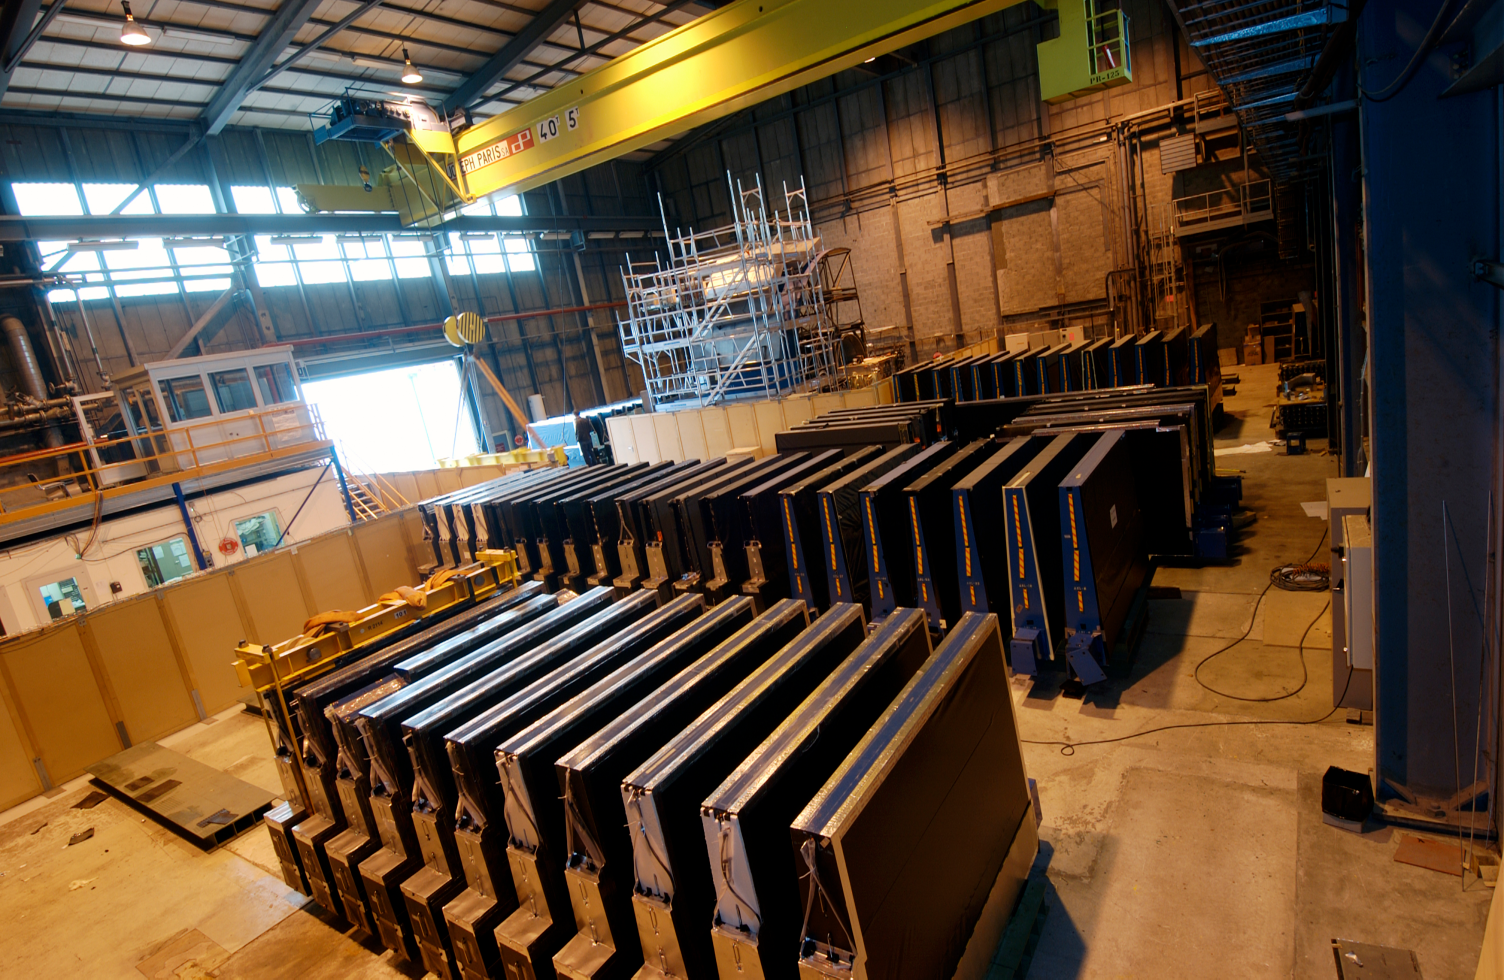
\includegraphics[width=0.495\textwidth]{figures/atlas/tile_pic.pdf}}
\caption{(a) Schematic representation of a TileCal module and its interface with the optical readout. (b)}
\label{fig:atlas:tile}
\end{figure}

An approximately projective geometry, shown in Fig. \ref{fig:atlas:tile_cells}, is provided by the grouping of the readout fibres into the PMTs: this defines a cell structure, and each cell has dimension $\Delta\eta \times \Delta\phi = $ 0.1 $\times$ 0.1 in the first two layers and $\Delta\eta \times \Delta\phi = $ 0.2 $\times$ 0.1 in the third layer. Special cells cover the gap region between the LB and the EB: the gap scintillators in the pseudorapidity region 1.0$<|\eta|<$1.2 and crack scintillators in the region 1.2$<|\eta|<$1.6, in front of the LAr end caps.

\begin{figure}[ht]
\centering
\subfigure{\includegraphics[width=0.7\textwidth]{figures/atlas/tile_cells.pdf}}
\caption{Layout of the projective geometry of the TileCal cells.}
\label{fig:atlas:tile_cells}
\end{figure}

The HEC shares the same cryogenic system as the ECal end caps, and covers the region with 1.5$<|\eta|<$3.2. Liquid argon is more resistant to radiation than the plastic scintillator used in TileCal, and is therefore the preferred choice in the end-cap region. Each side of the HEC consists of two wheels with outer radius of 2.03 m, and each wheel is composed by 32 identical modules. The electromagnetic signal produced in the LAr is collected by catodes on the plates. 

The FCal provides coverage in the forward region with 3.1$<|\eta|<$4.9. The FCal modules are located at high pseudorapidity, at a distance of 4.7 m along the $z$-axis from the interaction point.


\subsection{Muon Spectrometer}

\begin{figure}[ht]
\centering
\subfigure{\includegraphics[width=0.65\textwidth]{figures/atlas/muon}}
\caption{Layout of the ATLAS muon system. Figure from Ref. \cite{atlas:atlas}}
\label{fig:atlas:muon}
\end{figure}

\subsection{Luminosity Detectors}

\subsection{Luminosity Determination and Uncertainty}

\subsection{Trigger System}
\label{sec:cern:trigger}

\subsection{ATLAS Performance Summary}



\glsresetall
\glsunset{atlas}
\glsunset{cms}
\chapter{p-p Interactions and their Simulation}
\label{chap:event:MC}


\gls{pp} interactions at the \gls{lhc} are complicated processes that span very different energy scales. 
To interpret the \gls{lhc} data it is important to both 
develop a good understanding of the physics taking place during a \gls{pp} collision and also be able to simulate 
it, to allow a comparison of the observed data with data simulated based on a specific theory, first of all the \gls{sm}.
Section \ref{sec:ppint} focuses on the description of our understanding of a \gls{pp} collision, while Section \ref{sec:eventsimul} 
discusses the event-simulation process and the main \gls{mc} generators used in the \gls{atlas} Collaboration. 



\section{p-p Interactions}
\label{sec:ppint}

In hard-scattering processes, where the momentum transfer is much higher than the proton mass \cite{Butterworth:2012fj}, 
a \gls{pp} collision is easier to understand in terms of interactions between the constituents of the protons, quarks and gluons, 
collectively referred to as partons. A schematic view of \gls{pp} event is shown in Fig. \ref{fig:sim:pp2}. In this case, the interaction of a quark and a gluon leads to a final state with a Z boson and jets. 

\begin{figure}[h]
\begin{center}
%  \subfigure[]{
%    \label{fig:Comb_syst:pt}
    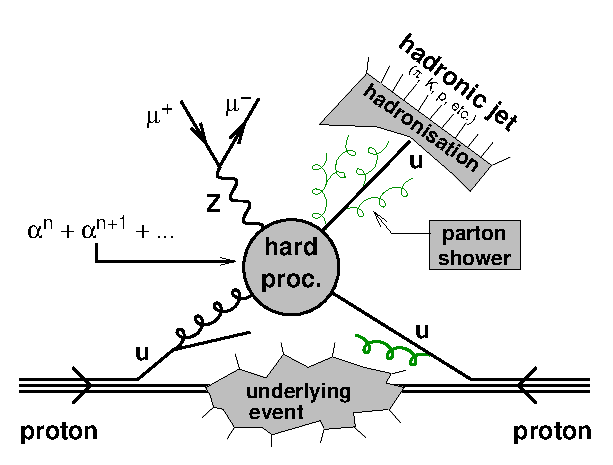
\includegraphics[width=0.58\textwidth]{figures/simul/ppcoll2}
%  }
\end{center}
 \caption{Schematic representation of a \gls{pp}, involving a quark-gluon scattering that leads to a final state consisting of a Z boson and a hard jet. Figure from Ref. \cite{Butterworth:2012fj}.}
  \label{fig:sim:pp2}
\end{figure}

As in can be understood from the figure, the hard process, which can be computed in perturbation theory, takes place between two of the proton partons; the probability that a gluon or a specific quark type takes part to the hard scattering is described the \glspl{partdf}, discussed in Section \ref{sec:ppint:hardscatter}. If the products of the hard scattering are quarks or gluons, after loosing energy by radiating other gluons (which in turn can generate quarks through gluon splitting) in the process of parton shower, they evolve into stable hadrons in the lower-energy hadronization process, which we can describe only through phenomenological models.
This picture is further complicated by the fact that also initial-state quarks and gluons can radiate. Also, the other partons not contributing to the hard scattering can interact, originating what is referred to as underlying event. 

\subsection{Factorization Theorem}
\label{sec:ppint:hardscatter}

The hard scattering between the partons inside the proton is in a kinematic regime where the \gls{qcd} coupling constant, $\alpha_s$, 
is small and therefore the partonic cross sections can be computed in perturbation theory. 
Thanks to the factorization theorem \cite{doi:10.1146}, the generic production cross section for a final state $X$ can be expressed in terms of the partonic cross section $\hat\sigma$ as:

\begin{equation}
  \label{eq:general-cross-section}
  \sigma(pp\rightarrow X) = \sum_{i,j} \int dx_1 dx_2\, 
     f_{i}(x_1,\mu_F^2)\, f_{j}(x_2,\mu_F^2)\, 
     \hat\sigma_{ij\rightarrow X}(x_1 x_2 s, \mu_R^2, \mu_F^2) \; .
\end{equation}
The $i$ and $j$ indexes run on all the possible partons, and $f_{i}(x_1,\mu_F^2)$ is the \gls{partdf} for the $i$-th parton, representing 
the distribution of probability for that parton to carry a fraction $x_1$ of the proton momentum when the proton is probed at a scale $\mu_F$
(factorization scale). $\hat\sigma_{ij\rightarrow X}$ is the partonic cross section, computer at the partonic center of mass energy \cmpart;   
it has to be noted that \cmpart is lower than the total center of mass energy, as its square is the product of square of the center of mass energy times
the fraction of the proton momentum that is carried by each of the two partons, $x_1$ and $x_2$. 
While, when considered at all orders in perturbative \gls{qcd}, the partonic cross section does not depend on $\mu_F$,
this dependence appears at any fixed order. $\hat\sigma$ depends also on the renormalization scale, $\mu_R$, which is the scale used for the evaluation of $\alpha_s$.



% factorization theorem 


%\begin{figure}[h]
%\begin{center}
%  \subfigure[]{
%    \label{fig:Comb_syst:pt}
%    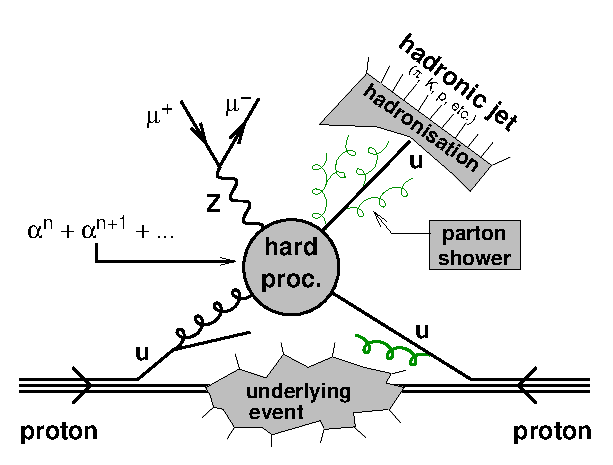
\includegraphics[width=0.48\textwidth]{figures/simul/ppcoll2}
%  }
%    \subfigure[]{
%    \label{fig:Comb_syst:pt}
%    \includegraphics[width=0.48\textwidth]{figures/simul/ppcoll}
%  }
%\end{center}
% \caption{Diagrammatic structure of a generic hard-scattering process. Figure from Ref. \cite{Campbell:2006wx}.}
%  \label{fig:sim:pp}
%\end{figure}

\subsection{Parton Density Functions}

The partons inside the proton can not be observed as free particles, and therefore their \glspl{partdf} can not be computed with
perturbative \gls{qcd}. In particular, for a given scale, it is not possible to predict theoretically the probability distribution 
of the momentum fraction. Instead, once the \glspl{partdf} are known for a certain scale, their energy evolution is 
determined by the equations derived independently by Dokshitzer \cite{Dokshitzer:1977sg} , Gribov and Lipatov \cite{Gribov:1972ri}, and Altarelli and Parisi \cite{ALTARELLI1977298} (DGLAP equations):

\begin{equation}
\begin{aligned}
\frac{\partial q(x,Q^2)}{\partial {\rm log}Q^2}~&=~\frac{\alpha_s}{2\pi}~\left( P_{qq} \otimes q~+~P_{qg} \otimes g \right) \, \\
\frac{\partial g(x,Q^2)}{\partial {\rm log}Q^2}~&=~\frac{\alpha_s}{2\pi}~\left( \sum_i P_{gq} \otimes (q_i+\bar{q}_i)~+~P_{gg} \otimes g \right) \; .
\label{eq:glap1}
\end{aligned}
\end{equation}

\noindent In the expressions above, $q(x,Q^2)$ and $g(x,Q^2)$ are the quark and gluon \gls{partdf} respectively, 
$P_{ij}$ describes the $i \to j$ parton splitting function
and $\otimes$ is a symbol for the convolution integral:
\begin{equation}
P \otimes f \equiv \int^1_x\frac{dy}{y}f_q(y)~P\left(\frac{x}{y}\right).
\end{equation}

As mentioned above, the $x$ dependence has to be extracted experimentally. This is done by several collaborations through fits (with typically 10 to 30 parameters) to data of \gls{dis}. As an example, Figure \ref{fig:sim:pp} shows the \gls{nlo} \glspl{partdf} obtained by the MSTW Collaboration for two different scales, Q$^2$ = 10 GeV$^2$ and Q$^2$ = 10$^4$ GeV$^2$. It is possible to notice how, with the increase of Q$^2$, the shape of the \glspl{partdf} changes to favor lower $x$ values. At low $x$ values the gluon \gls{pdf} is dominating (and this effect increases with Q$^2$), while for high $x$ values the \glspl{partdf} of the valence quarks are more relevant.

\begin{figure}[h]
\begin{center}
    \includegraphics[width=0.8\textwidth]{figures/simul/pdf}
\end{center}
\caption{MSTW 2008 \gls{nlo} \glspl{partdf} at Q$^2$ = 10 GeV$^2$ and Q$^2$ = 10$^4$ GeV$^2$. Figure from Ref. \cite{Martin:2009iq}.}
 \label{fig:sim:pp}
\end{figure}


\section{Event Simulation}
\label{sec:eventsimul}

\subsection{Matrix Element}

The factorization and renormalization scales are not predetermined, and are typically set to values related to the scale of the considered physical process. 
The impact of this subjective choice is taken into account by evaluating each production cross section at different scales (typically a variation of a factor two up and down), and assigning the difference as a systematic uncertainty on the cross section estimate.

\subsection{Parton Shower}

\subsection{Matching}

\subsection{Hadronization}

\section{MC Generators}

\section{Detector Simulation}

\section{Data-driven Corrections}

\glsresetall 
\glsunset{atlas}
\glsunset{cms}
\chapter{Event Reconstruction}
\label{sec:event:reco}

The particles produced in the \gls{pp} collisions in the center of the \gls{atlas} detector, interact with the detector material as discussed in Chapter \ref{chap:cern}. As a result of these interactions, electrical currents are recorded. \textit{Event reconstruction} is the process of recombining these digital signals and interpreting them as tracks and energy deposits in the calorimeters. A further step consists in analyzing the characteristics of the candidate tracks and calorimeter clusters and identify them as signs of the passage of specific particles.
This chapter describes the reconstruction and identification of the objects used in the analyses discussed in this thesis: tracks and vertices, electrons, muons, hadronic jets and missing transverse momentum. 


\subsection{Tracks and Primary Vertices}
\label{sec:reco:tracks}

In \gls{atlas} the identification of tracks from charged particles relies on the information collected by the \gls{id}. The tracking information is crucial to the reconstruction and identification of many types of particles, including electrons, muons, and the jest originating from the hadronization of a b-quark. The precision on the position measurement of the track depends on the granularity of the different subsystems of the \gls{id} and, since the \gls{id} is surrounded by a solenoidal magnetic field, the charged particles follow an helical trajectory. After the point of closest approach (perigee) to a given reference is defined, the trajectory of the track can be described by five parameters: 
\begin{equation}
\theta, \; \phi, \; q/p \; d_0, \; z_0 \;,
\end{equation}
\noindent where $\theta$ and $\phi$ are the azimuthal and polar angle, $q/p$ is the ratio of the charge of the track to the track momentum, and $d_0$ and $z_0$ are the distance to the point of closest approach in the transverse plane and along the $z$-axis. 

Primary tracks, originating from charged particles with a life time longer that $3 \times 10^{-11}$ s produced directly in the hard-scatttering vertex, are reconstructed with an inside-out approach \cite{Cornelissen:1020106}: the seed of the reconstruction are three hits in the silicon detector, and then compatible hits in the outer layers of the \gls{id} are added with a Kalman Filter \cite{citeulike:347166,Fruhwirth:1987fm}. The \gls{trt} segments that are not associated with primary tracks are used as starting point to reconstruct tracks from long-lived particles or from material interaction, with a back-tracking that extrapolates the \gls{trt} information to the pixel hits. 

Random groups of hits can be wrongly reconstructed as belonging to the helical trajectory of a track (\textit{fake tracks}). The amount of fake tracks increases with the increase of pile-up, and can be reduced by tightening the selection criteria of the track, at the expense of reconstruction efficiency. Three different selection criteria are used for the data collected in 2015 and 2016 (Loose, Loose-Primary and Tight-Primary), that differ in the requirements on the hits and holes (elements where a hit was expected but was not registered) in the different \gls{id} layers. The \textit{track reconstruction efficiency} is measured in \gls{mc} simulations as the ratio of the reconstructed tracks matched to a generated charged particle over the total number of generated charged particles. The reconstruction efficiency as a function of the track $\eta$ and \pt is shown in Fig. \ref{fig:obj:tracks} for Loose and Tight-Primary tracks.
 
\begin{figure}[ht]
\centering
\subfigure[]{\includegraphics[width=0.48\textwidth]{figures/objects/track1}}
\subfigure[]{\includegraphics[width=0.48\textwidth]{figures/objects/track2}}
\caption{Track reconstruction efficiency, evaluated by using minimum bias simulated events, as a function of truth $\eta$ (a) and \pt (b) for Loose and Tight Primary track selections.The bands indicate the total sstematic uncertainty. Figure from Ref. \cite{ATL-PHYS-PUB-2015-051}.}
\label{fig:obj:tracks}
\end{figure}

Tracks are the starting point for the identification of vertices. \glspl{pv} are reconstructed through a vertex fitting algorithm \cite{Fruhwirth:2007hz}, and then the vertex fitting algorithm identifies the vertex position and refits the tracks adding the constraint of the reconstructed interaction point. Once all the \glspl{pv} are reconstructed, the one with the highest sum of the squared transverse momenta of its associated tracks ($\sum_i^{N-tracks}p_{T,i}^2$) is identified as the hard scattering vertex, and $d_0$ and $z_0$ are recomputed with respect to its coordinates. The other vertices are named pile-up vertices, and their number is correlated  to the number of interactions per bunch crossing.


\subsection{Hadronic Jets}

The jet-finding algorithms of the $k_T$-family group together clusters that are close according to the metric $d_{i,j}$, defined as:

\begin{equation}
d_{i,j} = min\left( k_{T,i}^{2n}, k_{T,i}^{2n}  \right) \frac{\Delta R_{i,j}^2}{R^2},
\end{equation}

where $k_{T,i}$ is the transverse momentum of the cluster, $\Delta R_{i,j}$ is the angular distance defined as in \ref{eq:deltaR}, R is a fixed parameter, whose values sets the size of the jet, and n is the parameters that defines the kind of algorithm we are using and therefore the shape of the resulting jets. Besides the distance between clusters, the distance of a cluster form the beam is also defined:

\begin{equation}
d_{i,B} =  k_{T,i}^{2n}
\end{equation}

The $k_T$-family algorithms follow an iterative approach:
\begin{enumerate}
\item For each topocluster, the distances $d_{i,j}$ and $d_{i,B}$ are calculated
\item If $d_{i,B} < d_{i,j} \, \forall i \neq j $ the i-th cluster is defined as a jet
\item group together the two clusters i, j with the smallest $d_{i,j}$ among the remaining
\item Reiterate the procedure
\end{enumerate}

Depending on the value of the parameter n, we can distinguish different algorithms:
\begin{itemize}
\item $n=0$: Cambridge-Aachen. The grouping of the clusters depends only on geometrical considerations and not on their momentum. 
\item $n=1$: $k_T$ algorithm. Groups soft clusters first.
\item $n=-1$: $anti-k_T$ algorithm. Groups hard objects first; the shape of the jets is more regular than in the two previous cases and is a cone of radius R.
\end{itemize}

The choice of a particular algorithm results in different shapes of the jets, represented in fig. \ref{fig:jetsalg}. The standard algorithm used by \gls{atlas} is the $anti-k_T$ algorithm \cite{cacciari:antikt}.

\begin{figure}[h]
\includegraphics[width=\textwidth]{./figures/objects/jetsalg.pdf}
\caption[Shape of jets reconstructed with different algorithms]{Shape of jets reconstructed with different algorithms \cite{cacciari:antikt}.}
\label{fig:jetsalg}
\end{figure}


\subsubsection{Jets from B-hadrons}


\subsection{Electrons}

\subsection{Muons}

\subsection{Missing Transverse Momentum}

Particles that interact only weakly with the detector, such as neutrinos or BSM particles like neutralinos, are not reconstructed directly. 
Their presence is instead inferred by measuring the total momentum imbalance in the event. 

\begin{equation}
\met = \sqrt{(E_{X}^{miss})^{2}  +  (E_{Y}^{miss})^{2}},
\end{equation}

\begin{equation}
E_{X(Y)}^{miss} = E_{X(Y)}^{miss,e} +    E_{X(Y)}^{miss,\gamma} + E_{X(Y)}^{miss,\tau}    \nonumber \\
+ E_{X(Y)}^{miss,jets} + E_{X(Y)}^{miss,soft-terms}  +  E_{X(Y)}^{miss,\mu} 
\label{eq:etm} 
\end{equation}


\begin{equation}
\phi^{miss} = \arctan \left( \frac{E_Y^{miss}}{E_X^{miss}} \right)
\end{equation}





\glsresetall
\glsunset{atlas}
\glsunset{cms}
\chapter{Statistics Tool Box}
\label{chap:stat}

The data we collect is stochastic: quantum mechanics is not deterministic, so the particle content result of an interaction follows probabilistic laws. Furthermore, experimental effects need to be taken into account. Therefore, a proper statistical treatment is essential to extract quantitative statements from the observed data. This section describes the main statistical procedures that are used to obtain the results described in Chapter \ref{chap:strong_prod} and Chapter \ref{chap:ewk_prod}. The two main topics discussed are parameter estimation (Section \ref{sec:stat:pe}), that has the aim to determine the value of the input parameters that allows to best describe data, and hypothesis testing (Section \ref{sec:stat:ht}), that checks the plausibility of models against the observed data.

\section{Parameter Estimation}

\label{sec:stat:pe}



\subsection{Inclusion of Systematic Uncertainties}

\subsection{Profiled Likelihood Ratio}

\section{Hypothesis Testing}
\label{sec:stat:ht}


\subsection{The CLs Method}

\subsection{Asymptotic Approximation}



\glsresetall
\glsunset{atlas}
\glsunset{cms}
\chapter{Common Aspects to Multi-b SUSY Searches}
\label{chap:multib_general}

The main results presented in this thesis are the two analyses described in Chapter \ref{chap:strong_prod} and Chapter \ref{chap:ewk_prod}. While these analyses target two different \gls{susy} models they have many commonalities, since they both target \gls{susy} models leading to final states rich in b-jets and \met. This Chapter highlights these common aspects: Section \ref{sec:simplified_models} describes the philosophy of simplified models, used to design the signal models, Section \ref{sec:common_backgrounds} focuses on the background sources from \gls{sm} processes and how they are modeled in the analyses. 

\section{Simplified Models}
\label{sec:simplified_models}

\section{Analysis Strategy}

\section{Background Processes and their modelling}
\label{sec:common_backgrounds}

This section describes the main background processes from the \gls{sm} in the analysis regions and the way they are 
modeled in the analyses discussed in the next two chapters. In general, the modelling is based on \gls{mc} simulations for
all the backgrounds, except multi-jet which is emulated with a data-driven technique.
For the main background, pair production of top quark pairs, the shape of the different distributions is obtained from \gls{mc}
but the normalization is data-driven, derived in specifically designed \gls{cr} as described in Section \ref{sec:analyses:cr}.
Section \ref{sec:common_obj_def} focuses on the definition of the physic objects, and Section \ref{sec:common_syst} introduces the main sources of 
systematic uncertainties.

\subsection{Top quark pair production}

Top quark pair production constitutes the main source of background in all the analysis regions. 

\subsubsection{Truth-level classification: \ttbar decays}

\subsubsection{Truth-level classification: flavour of the associated jets}

\subsection{Control Regions}
\label{sec:analyses:cr}

\subsection{Single top quark production}

\subsection{Vector boson}

\subsection{Multi-bonson}

\subsection{\ttbar + V production}

\subsection{Multi-jet}


\section{Object Definition}
\label{sec:common_obj_def}

\section{Systematic Uncertainties}
\label{sec:common_syst}

\subsection{Experimental Systematic Uncertainties}

\subsection{Modeling Uncertainties} 


\glsresetall
\glsunset{atlas}
\glsunset{cms}
\chapter{Strong-production multi-b SUSY search}
\label{chap:strong_prod}


\section{Signal Model}

\section{Analysis Variables}


\section{Pre-fit Data-MC}


\section{Discovery Signal Regions}


\section{Exclusion Signal Regions}


\section{Results}


\section{Interpretation}

\section{Results in the Context of the ATLAS SUSY Group}
\glsresetall
\glsunset{atlas}
\glsunset{cms}
\chapter{Electroweak-production multi-b SUSY search}
\label{chap:ewk_prod}



\section{Signal Model}

\begin{figure}[htbp]
	\centering
	\includegraphics[width=0.35\textwidth]{figures/ewk_prod/varie/N1N1-hhGG-bbbb_Z}
	\caption{Diagram for the simplified model considered in the analysis. The primary interpretation of the analysis is the decay via Higgs bosons, but decays via varied branching ratios to $Z$ bosons are also studied. The production of the \hino\ occurs
via mass-degenerate pairs of charginos or neutralinos, which decay to the \ninoone\ and immeasurably low momentum particles.} 
	\label{fig:feyn}
\end{figure}

\subsection{Signal cross section}

%\section{Previous Limits}



\section{Discriminating variables}
\label{sec:ewk:sigbkg}

A key ingredient of the analysis is the reconstruction of the two Higgs bosons from the decay of the higgsinos.
Since this analysis targets events where both Higgs bosons decay to a $b\bar{b}$ pair, the reconstruction starts 
from four jets, which are chosen according to an ordering that favors $b$-tagged jets over non-tagged jets,
and then orders based on \pt. Practically, this results in the following criteria:
\begin{itemize}
\item If there are exactly four $b$-tagged jets in the event, those are used.
\item If there are more than four $b$-tagged jets, the selected ones are the four $b$-tagged jets with highest \pt.
\item If there are less than four $b$-tagged jets, the selected ones are the $b$-tagged jets and the non-tagged jets with highest \pt.
\end{itemize} 

Once the four jets have been selected, they are grouped in two pairs, each one constituting a candidate Higgs bosons. 
Different algorithms to pair the jets have been tested, and the chosen one is based on minimizing the angular separation 
between the two jets associated to the same Higgs boson candidate. 
In particular, the permutation chosen is the one that minimizes:
\begin{equation}
\dRmax = \mathrm{max}(\Delta R(h_1), \Delta R(h_2)) \; , \nonumber
\end{equation}

\noindent where $\Delta R(h)$ is the distance in the $\eta$--$\phi$ space between the two jets from the same candidate.
This choice has a good efficiency in reconstructing the Higgs bosons in the signal, 
and at the same time avoids creating artificial peaks in the background in correspondence of the Higgs boson mass. 
More details on the efficiency of the reconstruction and the comparison with other reconstruction algorithms are given in 
Appendix \ref{app:higgs}.

Beside the variables described in Section \ref{sec:common_variables}, a few other discriminating variables particularly 
effective for this signal model are described below.

\begin{description}
\item[Candidate Higgs bosons] The invariant mass of the two Higgs boson candidates built following the procedure outlined above 
is used as discriminating variable. In particular, we refer to m($h_1$) and m($h_2$) respectively for the mass of the Higgs candidate with 
the leading and subleading mass.

The variable \dRmax, defined in the previous section, is used to choose the pairing of the jets while reconstructing 
the Higgs boson candidates but also as a discriminating variable to separate signal and background. 

\item[Modified effective mass] In the signal model, only four jets come from the hard scattering process, and are therefore expected to be more energetic than the 
remaining jets in the event. Therefore the \meff definition is modified to include only the jets that are selected 
as originating from a Higgs boson; the modified definition is therefore:
\begin{equation}
\meffb = \sum_{i=1,..,4} {\pt}^{j_i} + \met \; , \nonumber
\end{equation}
\noindent where the sum runs over the jets selected according to the ordering procedure presented above.

\end{description}

The variables defined above, together with the ones defined in Section \ref{sec:common_variables},  
allow to identify a region of the phase space that is enriched in signal events. 
This study is performed after selecting events with high \met ($> 200$ GeV), at least four signal jets, at least three $b$-tagged jets, zero signal leptons, and \dphimin $>0.4$.

Figures \ref{fig:ewk:sig:1} and \ref{fig:ewk:sig:2}  show the distribution of the main kinematic variables for 
the sum of the \gls{sm} backgrounds and for different signal samples after these selections.
Figures \ref{fig:ewk:sig:mass_h1_min_dR} and \ref{fig:ewk:sig:mass_h2_min_dR} show the distribution of the mass of the Higgs 
candidate with the leading and subleading mass respectively. 
It can be appreciated that the distribution peaks at values around the Higgs mass for 
signals, while it is flatter for background. 
The distribution of \dRmax is shown in Figure \ref{fig:ewk:sig:dRmax_dR}. This variable assumes in general a lower value for 
signal events, in particular for the high-mass signals, where the Higgs bosons are produced with higher \pt and thus have 
more collimated decay products. Signal events also tend to have a lower number of signal jets, as can be observed in Figure 
\ref{fig:ewk:sig:jets_n}, and they occupy mostly the bins with three and four $b$-jets in the 
distribution of \nbjet, shown in Figure \ref{fig:ewk:sig:bjets_n}. 
The \met distribution, shown in Figure \ref{fig:ewk:sig:met}, displays the expected features: while signals with low-mass higgsinos 
have low \met values, the distribution tends to assume increasingly high values with the increase of the higgsino mass. 
A similar feature is shown in Figures \ref{fig:ewk:sig:meff_4bj} and \ref{fig:ewk:sig:mTb_min} for the \meffb and \mtb distributions respectively: 
the higher the higgsino mass in the signal, the more signal events differ from background events. 
While on the one hand this makes it easier to separate them from the \gls{sm} background, on the other hand the increase in signal mass 
implies a decrease in production cross-section, which will be the limiting factor in sensitivity to high-mass signals. 

\begin{figure*}[htbp]
\centering 
\subfigure[m($h_1$)]{\includegraphics[width=0.48\textwidth]{figures/ewk_prod/sig_bkg/hh_compare_mass_h1_min_dR.pdf}\label{fig:ewk:sig:mass_h1_min_dR}}
\subfigure[m($h_2$)]{\includegraphics[width=0.48\textwidth]{figures/ewk_prod/sig_bkg/hh_compare_mass_h2_min_dR.pdf}\label{fig:ewk:sig:mass_h2_min_dR}} \\
\subfigure[\dRmax]{\includegraphics[width=0.48\textwidth]{figures/ewk_prod/sig_bkg/hh_compare_dRmax_dR.pdf}\label{fig:ewk:sig:dRmax_dR}}
\subfigure[\meffb]{\includegraphics[width=0.48\textwidth]{figures/ewk_prod/sig_bkg/hh_compare_meff_4bj.pdf}\label{fig:ewk:sig:meff_4bj}}
\caption{Distribution of  the main kinematic variables in background and signal events after the selections described in the text.}
\label{fig:ewk:sig:1}
\end{figure*}

\begin{figure*}[htbp]
\centering
\subfigure[\njet]{\includegraphics[width=0.48\textwidth]{figures/ewk_prod/sig_bkg/hh_compare_jets_n.pdf}\label{fig:ewk:sig:jets_n}}
\subfigure[\nbjet]{\includegraphics[width=0.48\textwidth]{figures/ewk_prod/sig_bkg/hh_compare_bjets_n.pdf}\label{fig:ewk:sig:bjets_n}}\\
\subfigure[\met]{\includegraphics[width=0.48\textwidth]{figures/ewk_prod/sig_bkg/hh_compare_met.pdf}\label{fig:ewk:sig:met}}
\subfigure[\mtb]{\includegraphics[width=0.48\textwidth]{figures/ewk_prod/sig_bkg/hh_compare_mTb_min.pdf}\label{fig:ewk:sig:mTb_min}}
\caption{Distribution of  the main kinematic variables in background and signal events after the selections described in the text.}
\label{fig:ewk:sig:2}
\end{figure*}

\FloatBarrier

\section{Signal regions}
\label{sec:ewk:SR}

This section describes the optimization of the \glspl{sr}. 
The high \gls{br} of the Higgs boson to a $b\bar{b}$ pair (58\%) makes a channel with at least three $b$-jets very 
promising to look for signal models 
in which both higgsinos decay to h+$\gravino$. 
Therefore, the analysis selections are optimized to maximize the expected sensitivity to signals leading to $hh+\met$ 
and all the \glspl{sr} require both boson candidates to have masses compatible with the Higgs mass (the specific mass range is chosen during the optimization). 
%The target signal model is shown in Figure \ref{fig:opt_sighh4b}.

\subsection{Multi-bin regions}
\label{sec:ewk:multibin}

The optimization of the multi-bin \glspl{sr} aims at constructing several orthogonal \glspl{sr}, that can be statistically combined. 
The optimization strategy follows these steps:
\begin{enumerate}
\item A first variable (var$_1$) is chosen to define a coarse binning. 
    This variable should provide both a good signal-to-background discrimination and discrimination between signal 
    with different higgsino masses.
\item For each of these bins in var$_1$, a \gls{cr} is defined to normalize the \ttbar background in a kinematic regime close to the corresponding \gls{sr}.
\item Each bin based on var$_1$ is further split based on a second variable, var$_2$ (in this case all the bins based on the second variable share the same \gls{cr}).
\item The selections on the remaining kinematic variables are optimized independently in each var$_1$ bin (i.e. all the regions sharing the same 
\gls{cr} have the same selections on all the variables except var$_2$).
\end{enumerate}

\noindent As described above, var$_1$ must be able to provide at the same time a good separation between signal and background 
and a good separation between signals with different \hino masses. 
The latter is necessary in order to be able to optimize each bin in var$_1$ based on a different signal mass, 
providing in the end a good sensitivity to the entire mass spectrum. 
In order to understand which variable works best for this scope, the separation algorithm provided by the TMVA toolkit \footnote{TMVA is a toolkit designed for multivariate analyses, this in not the case here: it's only used as a quick way to access the discrimination power of the individual variables.} \cite{Hocker:2007ht} is used, defined as:

\begin{equation}
          \mathrm{separation} = \frac{1}{2} \int\frac{\left(f_s(x) - f_b(x)\right)^2}{f_s(x) + f_b(x)} dx \; , 
\label{eq:separation}
\end{equation}
\noindent where $f_s$ and $f_b$ are the signal and background \glspl{pdf} of $x$. 

The separation provided by the most promising analysis variables between background and 
signals with m(\hino)=300, 500 and 800 GeV is shown in Figure \ref{fig:ewk:separation}.
It is possible to see that \meffb is the best variable for our requirements (even if there are individual bins where this is not the case). 

\begin{figure}[htpb]
\begin{center}
%\subfigure[]{\includegraphics[width=0.43\textwidth]{figures/ewk_prod/separation/saparation_Dphi.pdf}}
\subfigure[\meffb]{\includegraphics[width=0.43\textwidth]{figures/ewk_prod/separation/saparation_meff_4bj.pdf}}
\subfigure[\dRmax]{\includegraphics[width=0.43\textwidth]{figures/ewk_prod/separation/saparation_dR_max.pdf}}\\
\subfigure[\nbjet]{\includegraphics[width=0.43\textwidth]{figures/ewk_prod/separation/saparation_Njets.pdf}}
\subfigure[\njet]{\includegraphics[width=0.43\textwidth]{figures/ewk_prod/separation/saparation_Nb_jets.pdf}}\\
\subfigure[\mtb]{\includegraphics[width=0.43\textwidth]{figures/ewk_prod/separation/saparation_mTbmin.pdf}}
\subfigure[\met]{\includegraphics[width=0.43\textwidth]{figures/ewk_prod/separation/saparation_MET.pdf}}\\
%\subfigure[]{\includegraphics[width=0.43\textwidth]{figures/ewk_prod/separation/saparation_MET_sig.pdf}}
\caption{Separation offered by different analysis variables. The separation is defined as in Equation \ref{eq:separation}.}
\label{fig:ewk:separation}
\end{center}
\end{figure}

Three regular bins with a width of 150 GeV each are defined in \meffb. 
The edges of the bins are defined starting from the one with the highest value. 
As it has already been discussed in Section \ref{sec:ewk:sigbkg},
signals with high m(\hino) have kinematic features that distinguish them clearly from the background, 
but at the same time a low cross-section (e.g. for m($\tilde{H}$) = 800 GeV, the cross-section is about 3 fb). 
This makes it more convenient to define the selection that maximize the expected significance for a high-mass benchmark point (800 GeV) 
as a single-bin region, to concentrate as much as possible the signal events in one single \gls{sr}, 
instead of diluting it in several \glspl{sr}. % to try to exploit shape information.
The optimal selection for the high-m(\hino) benchmark signal occupies the highest \meffb bin,
and is determined my maximizing the expected significance over all the other discriminating variables,
leading to the selection:
\meffb $>$ 1100 GeV, \mtb$>$130 GeV, \dRmax $<$ 1.4, \met $>$200, $\geq$ 3 $b$-jets (77\% \gls{op}), 
4-5 jets, m($h_1$) in the range 110--150 GeV, and m($h_2$) in the range 90--140 GeV.

Considering the separation power of the different variables shown in Figure  \ref{fig:ewk:separation} 
and the signal-to-background comparison in Figure \ref{fig:ewk:sig:1}, 
\dRmax is chosen as second binning variable. 
%to gain signal acceptance also for signals less boosted than the 800 GeV mass one, where the angular separation between the two $b$-jets originating from the same higgs is larger.
Once the selections for the high-\meffb \gls{sr} have been defined, 
a similar procedure is repeated for the other \meffb ranges: 600-850 GeV and 850-1100 GeV. 
These two bins with lower \meffb are also split according to the number of $b$-jets: exactly 3 and $\geq$4. 
The two bins in $b$-jet multiplicity are optimized separately. 
For each of the four remaining regions, the following steps are taken:

\begin{enumerate}
\item Optimize for one specific signal benchmark: \mhino = 300, 500 GeV for the 600--850 and 850--1100 GeV \meffb bins respectively.
\item  Where possible with a loss in significance $<$ 15\%, the selections are made uniform. 
This results to be the case for the m($h_1$) and m($h_2$) ranges, for the selection in \met, for the first bin in \dRmax, 
and for the number of jets. In the case of this last variable, it is possible to make it uniform (4--5 jets) 
without consistent loss in sensitivity in all bins except in the 4b-meff2 bin, where a veto on a 6th jet is penalizing; 
in this region, the selection on the number of jets is 4--6.
\item Use \dRmax to define further bins.
\end{enumerate}

It is found that a second bin in \dRmax is really helpful only in the regions with low and intermediate \meffb, and  $\geq$ 4 $b$-jets. 
This is because the highest \meffb region is particularly sensitive to high-mass signals, where \dRmax is small. 
For signals with lower masses, the signal-to-background ratio in regions with exactly 3 $b$-jets and high \dRmax is too low, 
while the requirement of a fourth $b$-jet suppresses the \gls{sm} background further and gives good sensitivity 
also to the kinematic region with higher \dRmax.
The selections that define the \glspl{sr} are summarized in Table \ref{tab:SR}.

\begin{table}[htbp]
\begin{center}
%\resizebox{1.\textwidth}{!}{
\renewcommand{\arraystretch}{1.1}
\begin{tabular}{|l|c|c|c|}
\toprule
  & SR-3b-meff1-A & SR-3b-meff2-A & SR-3b-meff3-A\\
 \hline
\nbjet &  $=$3 &  $=$3 &  $\geq$3 \\
 \hline
\met & \multicolumn{3}{c|}{$>$ 200}\\
\hline
\dphimin    & \multicolumn{3}{c|}{$>$0.4}\\
 \hline
\njet &  4--5 &  4--5 &  4--5 \\
 \hline
\mtb &  $>$150 &  $>$150 &  $>$130 \\
 \hline
$m(h_1)$ &    \multicolumn{3}{c|}{110--150}\\
 \hline
$m(h_2)$ &    \multicolumn{3}{c|}{90--140}\\
 \hline
\dRmax &  0.4--1.4 &  0.4--1.4 &  0.4--1.4 \\
 \hline
\meffb &  600--850 &  850--1100 &  $>$1100  \\
\bottomrule
\end{tabular} 

\vspace{0.4cm}

\begin{tabular}{|l|c|c|c|c|}
\toprule
   & SR-4b-meff1-A & SR-4b-meff1-B & SR-4b-meff2-A & SR-4b-meff2-B  \\
 \hline
\nbjet &  $\geq$4 &  $\geq$4 &  $\geq$4 &  $\geq$4 \\
 \hline
\met & \multicolumn{4}{c|}{$>$ 200}\\
\hline
\dphimin    & \multicolumn{4}{c|}{$>$0.4}\\
 \hline
\njet & 4--5 &  4--5 &  4--6 &  4--6 \\
 \hline
\mtb &   - & - & - & -  \\
 \hline
$m(h_1)$ &    \multicolumn{4}{c|}{110--150}\\
 \hline
$m(h_2)$ &    \multicolumn{4}{c|}{90--140}\\
 \hline
\dRmax &   0.4--1.4 &  1.4--2.4 &  0.4--1.4 &  1.4--2.4\\
 \hline
\meffb &  600--850 &  600--850 &  850--1100 &  850--1100 \\
\bottomrule
\end{tabular} 
%}
\caption{Signal region definitions for the high-mass analysis. The units of \met, \mtb, $m(h_1)$, $m(h_2)$, and \meffb are GeV. 
Table from Ref. \cite{Aaboud:2018htj}.
%These variables are defined in Section~\ref{high_event_selection}.
}
\label{tab:SR}
\end{center}
\end{table}

\subsection{Cut-and-count regions}

The analysis strategy described in Section \ref{sec:ewk:multibin} leads to a good sensitivity for exclusion across the entire mass spectrum, 
but the constraint of building orthogonal regions makes it hard to have a high discovery significance 
for signals with intermediate masses. 
To solve this problem cut-and-count \glspl{sr} are defined as well, with the goal of
providing robust regions capable of discovering \gls{susy} signatures, 
and allowing an easier reinterpretation of the results.

The upper selection on \meffb, that makes the different \glspl{sr} orthogonal, 
is the one limiting the most the sensitivity of the individual \glspl{sr}.
In the exclusion fit this is not a problem, as the sensitivity lost in one bin is recovered in the neighbouring one. 
To define the discovery regions, all the individual \glspl{sr} are considered without the upper cut on \meffb
and the expected significance for some benchmark signal models is computed in each. 
The expected significance is computed as discussed in Section \ref{sec:example_sr}, 
assuming 36.1 \ifb{} of data and a normalization uncertainty of 30\% on the background. 

Figure \ref{fig:ewk:disc_sig} shows the expected significance for all the multi-bin analysis regions once the upper \meffb 
selection is removed. 
Using only the modified versions of SR-4b-meff1-A, referred to as SR-4b-meff1-A-disc, 
and SR-3b-meff3 (orange and green line respectively in the figure) allows us to have good expected sensitivity for 
all the signal considered.  
This is always larger than three standard deviations for 
signals with \mhino  
in the 300--600 GeV range, and $\approx$ 2.5 standard deviations for the signal with $\mhino=800$ GeV. 
The definition of SR-4b-meff1-A-disc is reported in Table \ref{tab:SR-disc}.

\begin{figure*}[htbp]
\centering
\includegraphics[width=0.7\textwidth]{figures/ewk_prod/discovery/significances_hh_regions.pdf}
\caption{Expected significance for the multi-bin regions after removing the upper \meffb selection. 
\label{fig:ewk:disc_sig}
}
\end{figure*}

\begin{table}[htbp]
\begin{center}
\renewcommand{\arraystretch}{1.1}
\begin{tabular}{|l|c|}
\toprule
   & SR-4b-meff1-A-disc \\
 \hline
\nbjet &  $\geq4$\\
 \hline
\met & $>$ 200\\
\hline
\dphimin    &$>$0.4\\
 \hline
\njet &  4--5\\
 \hline
\mtb &  - \\
 \hline
$m(h_1)$ &    110--150\\
 \hline
$m(h_2)$ &   90--140\\
 \hline
\dRmax &  0.4--1.4 \\
 \hline
\meffb &  $>600$ \\
\bottomrule
\end{tabular} 
%}
\caption{Definition of the high-mass analysis  SR-4b-meff1-A-disc. The units of \met, \mtb, $m(h_1)$, $m(h_2)$, and \meffb are GeV. 
Table from Ref. \cite{Aaboud:2018htj}.
%These variables are defined in Section~\ref{high_event_selection}.
}
\label{tab:SR-disc}
\end{center}
\end{table}


\section{Control and validation regions}
\label{sec:ewk:CRVR}

The \ttbar background is normalized in specifically designed \glspl{cr}.
A different \gls{cr} is built for each bin in \meffb and $b$-tagging multiplicity. 
These \glspl{cr} are built using side-bands both in m($h_1$) and m($h_2$). 
The extrapolation between \glspl{cr} and \glspl{sr} is tested in the \glspl{vr}, which take advantage of events
where only one between m($h_1$) and m($h_2$) is in the \gls{sr} mass range, 
as shown in Figure \ref{fig:binning_crvr}.

\begin{figure}[htbp]
	\centering
	\includegraphics[width=0.490\textwidth]{figures/ewk_prod/varie/schema-1}
	\caption{The division of signal, control, and validation regions using the $m(h_1)$ and $m(h_2)$ variables in the high-mass analysis.}
	\label{fig:binning_crvr}
\end{figure}

Some of the selections of the \glspl{sr} are modified when moving to the \glspl{cr} or \glspl{vr}
 to allow enough events and low signal contamination.
The main extrapolation between \glspl{cr} and \glspl{sr} are:

\begin{itemize}
\item In the \gls{cr}, both m($h_1$) and m($h_2$) are required to be outside the \gls{sr} mass ranges.
\item \dRmax is relaxed to $<$4 (or removed).
\item \mtb is relaxed by 30 GeV in 3b-meff3 and by 50 GeV in 3b-meff1 and 3b-meff2.
\end{itemize}

To allow enough events in the \glspl{vr}, the \glspl{vr} are non orthogonal. Since these regions do not enter the fit, but are only used to validate the background prediction, non-orthogonality is not an issue here. 
The selections that remove the orthogonality between the different \glspl{vr} are:
\begin{itemize}
\item The edges of \meffb selection are relaxed by 50 GeV up and down.
\item The edges of the \dRmax bins are relaxed and, when two \dRmax bins are present for the same type of regions, they are partially overlapping.
\end{itemize}

With respect to the \glspl{sr}, the \mtb selection in the \glspl{vr} (where present) is relaxed as well by 50 GeV. 
Note that \glspl{cr} and \glspl{vr} do not have extrapolation in \nbjet or \njet with respect to the SRs.
The selections for all the \glspl{cr} and \glspl{vr} are summarized respectively in Tables \ref{tab:ewk:CR} and \ref{tab:ewk:VR}.


\begin{table}[htbp]
\begin{center}
%\resizebox{0.75\textwidth}{!}{
\renewcommand{\arraystretch}{1.1}
\begin{tabular}{|l|c|c|c|c|c|}
\toprule
  & CR-3b-meff1 & CR-3b-meff2 & CR-3b-meff3 & CR-4b-meff1 & CR-4b-meff2 \\
 \hline
\nbjet &  $=$3 &  $=$3 &  $\geq$3 &  $\geq$4 &  $\geq$4 \\
 \hline
\met  & \multicolumn{5}{c|}{$>$ 200}\\
 \hline
\dphimin  & \multicolumn{5}{c|}{$>$0.4}\\
 \hline
\njet &  4--5 &  4--5 &  4--5 &  4--5 &  4--6 \\
 \hline
\mtb &  $>$100 &  $>$100 &  $>$100 & - & - \\
 \hline
$m(h_1)$, $m(h_2)$  &  \multicolumn{5}{c|}{ ($m(h_1)<$80, $m(h_2)<$80) or ($m(h_1)>$150, $m(h_2)<$80) or ($m(h_1)>$150, $m(h_2)>$140)    }\\
 \hline
\dRmax &  0.4--4 &  0.4--4 &  0.4--4 &  0.4--4 &  $\geq$ 0.4 \\
 \hline
\meffb &  600--850 &  850--1100 &  $>$1100 &  600--850 &  850--1100 \\
\bottomrule
\end{tabular} 
%} 
\caption{Control region definitions in the high-mass analysis. The units of \met, \mtb, $m(h_1)$, $m(h_2)$, and \meffb are GeV. 
Table from Ref. \cite{Aaboud:2018htj}.
%These variables are defined in Section~\ref{high_event_selection}.
}
\label{tab:ewk:CR}
\end{center}
\end{table}

\begin{table}[htbp]
\begin{center}
\renewcommand{\arraystretch}{1.1}
%\resizebox{1\textwidth}{!}{
\begin{tabular}{|l|c|c|c|}
\toprule
  & VR-3b-meff1-A & VR-3b-meff2-A & VR-3b-meff3-A \\
 \hline
\nbjet &  $=$3 &  $=$3 &  $\geq$3  \\
 \hline
\met  &  \multicolumn{3}{c|}{$>$200}\\
 \hline
\dphimin &  \multicolumn{3}{c|}{$>$0.4}\\
 \hline
\njet &  4--5 &  4--5 &  4--5 \\
 \hline
\mtb  & $>$120   & $>$100  & $>$80 \\
 \hline
$m(h_1)$, $m(h_2)$  &  \multicolumn{3}{c|}{   (80<$m(h_1)$<150, $m(h_2)$<80) or ($m(h_1)$>150, 90<$m(h_2)$<140)   }\\
 \hline
\dRmax &  0.4--1.5 &  0.4--1.7 &  0.4--1.7  \\
 \hline
\meffb   & 550--900   & 800--1150  & $>$1050    \\
\bottomrule
\end{tabular} 

\vspace{0.4cm}

\begin{tabular}{|l|c|c|c|c|}
\toprule
  &  VR-4b-meff1-A & VR-4b-meff1-B & VR-4b-meff2-A & VR-4b-meff2-B \\
 \hline
\nbjet &   $\geq$4 &  $\geq$4 &  $\geq$4 &  $\geq$4 \\
 \hline
\met  &  \multicolumn{4}{c|}{$>$200}\\
 \hline
\dphimin &  \multicolumn{4}{c|}{$>$0.4}\\
 \hline
\njet &   4--5 &  4--5 &  4--6 &  4--6 \\
 \hline
\mtb   &  \multicolumn{4}{c|}{-}\\
 \hline
$m(h_1)$, $m(h_2)$  &  \multicolumn{4}{c|}{   (80<$m(h_1)$<150, $m(h_2)$<80) or ($m(h_1)$>150, 90<$m(h_2)$<140)   }\\
 \hline
\dRmax &   0.4--1.7 &  1.4--3 &  0.4--1.7 &  1.4--3 \\
 \hline
\meffb   &  550--900  & 550--900  & 800--1150  & 800--1150  \\
\bottomrule
\end{tabular} 
%} 
\caption{Validation region definitions in the high-mass analysis. The units of \met, \mtb, $m(h_1)$, $m(h_2)$, and \meffb are GeV. 
Table from Ref. \cite{Aaboud:2018htj}.
%These variables are defined in Section~\ref{high_event_selection}.
}
\label{tab:ewk:VR}
\end{center}
\end{table}

\section{Background composition}
\label{sec:ewk:bkgcomp}

The pre-fit background composition of the analysis regions is show in Figures \ref{fig:bkgcomp_hh3b} and \ref{fig:bkgcomp_hh4b}.
It is possible to see how \ttbar is the dominant background in all the \glspl{sr}.
%The \glspl{cr} and the \glspl{vr} have a high \ttbar purity by construction. 
%, since they are designed to respectively normalize this background and validate the extrapolation of this normalization to 
%a phase space closer to the \glspl{sr}.
% chiara: change, sentence from paper
The subdominant background contributions are $Z(\to \nu\nu)$+jets and $W(\to \ell\nu)$+jets events.
%where for W+jets events the lepton is electron or muon that is not reconstructed or a hadronically decaying $\tau$-lepton. 
%In the 1-lepton \glspl{sr}, the subdominant backgrounds are single-top, \ttbar+W and \ttbar+Z.
Figures \ref{fig:ttcomp_hh3b} and \ref{fig:ttcomp_hh3b} show the decay type of the \ttbar background,
while the heavy-flavor composition of the jets that are produced together with the \ttbar pair is shown 
in Figures \ref{fig:HFcomp_hh3b} and \ref{fig:HFcomp_hh4b}.

\begin{figure}[htbp]
\includegraphics[width=\textwidth]{figures/ewk_prod/comp_plots/hh_3b_bkg.pdf}
\caption{Background composition in the regions with exactly three $b$-jets.}
	\label{fig:bkgcomp_hh3b}
\end{figure}

\begin{figure}[htbp]
\includegraphics[width=\textwidth]{figures/ewk_prod/comp_plots/hh_4b_bkg.pdf}
\caption{Background composition in the regions with at least four $b$-jets.}
	\label{fig:bkgcomp_hh4b}
\end{figure}

\begin{figure}[htbp]
\includegraphics[width=\textwidth]{figures/ewk_prod/comp_plots/hh_3b_tt.pdf}
\caption{Decay mode of the \ttbar background in the regions with exactly three $b$-jets.}
	\label{fig:ttcomp_hh3b}
\end{figure}

\begin{figure}[htbp]
\includegraphics[width=\textwidth]{figures/ewk_prod/comp_plots/hh_4b_tt.pdf}
\caption{Decay mode of the \ttbar background in the regions with at least four $b$-jets.}
	\label{fig:ttcomp_hh4b}
\end{figure}

\begin{figure}[htbp]
\includegraphics[width=\textwidth]{figures/ewk_prod/comp_plots/hh_3b_HF.pdf}
\caption{Heavy-flavor composition of the \ttbar background in regions with exactly three $b$-jets.}
	\label{fig:HFcomp_hh3b}
\end{figure}

\begin{figure}[htbp]
\includegraphics[width=\textwidth]{figures/ewk_prod/comp_plots/hh_4b_HF.pdf}
\caption{Heavy-flavor composition of the \ttbar background in regions with at least four $b$-jets.}
	\label{fig:HFcomp_hh4b}
\end{figure}

\FloatBarrier

\section{Comparison between data and simulation}
\label{sec:ewk:dataMC}

The modeling of the main kinematic variables is very similar to what discussed in Section \ref{sec:strong:dataMC} 
for the gluino search, as the few differences in object definitions are not enough to 
lead to a substantial change in the agreement between data and simulation. 
This section therefore focuses on the variables specific to Higgs boson reconstruction.
The comparison between data and simulation for the variables already shown in Section \ref{sec:strong:dataMC} but with the object definitions 
specific to this analysis are shown in Appendix \ref{app:ewk:datamc}.
There is nevertheless a notable exception: in the analysis described in this chapter, the agreement between data and simulation in the 
distribution of the number of $b$-jets is improved, as can be appreciated comparing Figure \ref{fig:strong:datamc0L:bjets_n} with Figure \ref{fig:ewk:datamc_bjets}.
This is the result of the improvement in the $b$-tagging calibration: as discussed in Section \ref{sec:obj:btaggingcalib}, 
the calibration of $c$-jets used in this analysis is based on \ttbar events, rather than on $W+c$ events as in the gluino analysis.
The other important difference with respect to the strong-production analysis is that in this case the analysis is performed 
only in regions with a lepton veto; it is not therefore sensitive to the mis-modelling in the 1-lepton channel discussed in Section 
\ref{sec:strong:kinrw} and no kinematic reweighting is required. 

As can be observed in Figure \ref{fig:ewk:datamc_a}, all the variables specific to this analysis show a good 
agreement between data and the simulation. 

\begin{figure*}[htbp]
\centering 
%\subfigure[\nbjet]{
\includegraphics[width=0.45\textwidth]{figures/ewk_prod/data_mc/0L_3bin/data_mc_bjets_n.pdf}
%\label{fig:ewk:datamc:bjets_n}}\\
\caption{Comparison of the number of $b$-jets between data and simulation in the preselection described in the text.
}
\label{fig:ewk:datamc_bjets}
\end{figure*}

\begin{figure*}[htbp]
\centering 
\subfigure[m($h_1$)]{\includegraphics[width=0.45\textwidth]{figures/ewk_prod/data_mc/0L_3bin/data_mc_mass_h2_min_dR.pdf}
\label{fig:ewk:datamc:mass_h2_min_dR}}
\subfigure[m($h_2$)]{\includegraphics[width=0.45\textwidth]{figures/ewk_prod/data_mc/0L_3bin/data_mc_mass_h2_min_dR.pdf}
\label{fig:ewk:datamc:mass_h2_min_dR}}\\
\subfigure[\dRmax]{\includegraphics[width=0.45\textwidth]{figures/ewk_prod/data_mc/0L_3bin/data_mc_dRmax_dR.pdf}
\label{fig:ewk:datamc:dRmax_dR}}
\subfigure[\meffb]{\includegraphics[width=0.45\textwidth]{figures/ewk_prod/data_mc/0L_3bin/data_mc_meff_4bj.pdf}
\label{fig:ewk:datamc:pt_meff_4bj}}
\caption{Comparison between data and simulation in the preselection described in the text.
}
\label{fig:ewk:datamc_a}
\end{figure*}

\clearpage



\section{Systematic Uncertainties}
\label{sec:ewk:syst}

The effect of the systematic uncertainties discussed in Sections \ref{sec:common_syst} and \ref{sec:common_backgrounds} 
is summarized in Figure \ref{fig:syst_etmiss}, which shows the relative size of each group of systematics after the fit in the 
\glspl{cr}. 
The meaning of each group of systematics is the same as discussed for the gluino search in Section \ref{sec:strong:syst}.


% \gls{jes} (that has a relative impact on the expected background between 4 and 35\% in the different \glspl{sr}), \gls{jer} (0-26\%) and the uncertainties on the b-tagging efficiency and mistagging rate (3-24\%).
%  \ttbar background, whose impact ranges between 5 and 76\%).

\begin{figure}[htbp]
	\centering
	\includegraphics[width=0.85\textwidth]{figures/ewk_prod/etmiss_misc/High-MET-syst.pdf}
	\caption{Relative systematic uncertainties in the background estimate for the high-mass analysis. The individual uncertainties can be correlated, such that the total background uncertainty is not necessarily their sum in quadrature. Figure from Ref. \cite{Aaboud:2018htj}. 
	} 
	\label{fig:syst_etmiss}
\end{figure}

\section{Results}
\label{sec:ewk:results}

Figure \ref{fig:ewk:pullCR} shows the comparison between data and simulation in the \glspl{cr} before the fit (top panel)
and the scale factor for the \ttbar background that is derived from the fit in the \glspl{cr} (bottom panel).
If we compare with the equivalent result for the gluino search, in Figure \ref{fig:pullCR}, it is possible 
to see that on average the \ttbar scale factors have values closer to one. 
This is again because of the improvement in the $b$-tagging calibration of $c$-jets was implemented in this analyses. 
The fit in the \glspl{cr} is extrapolated to the \glspl{vr} and to the \glspl{sr}. 

The post-fit data-\gls{mc} agreement in the \glspl{vr} is shown in Figure \ref{fig:ewk:pullVR}: the top panel of this figure 
shows the post-fit predicted yields in each of the \glspl{vr} and the data yields, while the bottom panel quantifies the 
difference between observed data and predictions in terms of the significance, defined as in Ref. \cite{Choudalakis:2011okv}. 
Note that this is different from the pull definition adopted in the gluino search. 
The closure in the \glspl{vr} is good: all the bins have discrepancies with significance lower than 0.8. 

The results in the \glspl{sr} are shown in Figure \ref{fig:ewk:pullSR}. As in Figure \ref{fig:ewk:pullVR}, the top panel shows the 
predicted and observed yields in each \gls{sr}, and the bottom panel the significance of the discrepancy. 
No significant excess is observed and the observations are in agreement with the \gls{sm} predictions. 
The numerical results of the background-only fit extrapolated to the \glspl{sr} are presented in Table \ref{tab:ewk:yieldsSR},
where the background prediction is also broken down by component. 
This table shows also the total background prediction before the fit in the \glspl{cr}, which is labeled as ``MC-only background''.


\begin{figure}[htbp]
	\centering
	\includegraphics[width=0.9\textwidth]{figures/ewk_prod/etmiss_results/histpull_pulls_in_CR_qcdStrong}
	\caption{Event yields in control regions and related \ttbar\
          normalization factors after the background-only fit for
          %Inputs and results of the likelihood fit in the control
          %regions of
          the high-mass analysis. The upper panel shows 
		the observed number of events and the predicted background yield before the fit.
		All uncertainties  shown in Figure \ref{fig:syst_etmiss} are included in the uncertainty band. The background category $\ttbar+X$ includes $\ttbar W/Z$, $\ttbar H$, and $\ttbar \ttbar$ events.  
		The $\ttbar$ normalization is obtained from the fit
                and is displayed in the bottom panel. Figure from Ref. \cite{Aaboud:2018htj}.
	} 
	\label{fig:ewk:pullCR}
\end{figure}


\begin{figure}[htbp]
	\centering
	\includegraphics[width=0.9\textwidth]{figures/ewk_prod/etmiss_results/histpull_pulls_in_VR_qcdStrong}
	\caption{Results of the background-only fit extrapolated to the \glspl{vr}. 
	    The $\ttbar$ normalization is obtained from the fit to the \glspl{cr} shown in Figure~\ref{fig:ewk:pullCR}. The upper panel shows 
		the observed number of events and the predicted background yield. The bottom panel shows the significance of any disagreement between the data and the background model, computed as in Ref. \cite{Choudalakis:2011okv}.
		All uncertainties  shown in Figure \ref{fig:syst_etmiss} are included in the 
		uncertainty band. The background category $\ttbar+X$ includes $\ttbar W/Z$, 
		$\ttbar H$, and $\ttbar \ttbar$ events. Figure from Ref. \cite{Aaboud:2018htj}.}
	\label{fig:ewk:pullVR}
\end{figure}

\begin{figure}[htbp]
	\centering
	% \subfigure[]{\includegraphics[width=0.65\textwidth]{figures/etmiss_results/histpull_pulls_in_CR_qcdStrong}\label{fig:pullCR}}\\
	\includegraphics[width=0.9\textwidth]{figures/ewk_prod/etmiss_results/histpull_pulls_in_SR_qcdStrong}
	\caption{Results of the background only fit extrapolated to the \glspl{sr}. 
	The $\ttbar$ normalization is obtained from the fit to the CRs shown in Figure~\ref{fig:pullCR}. The data in the  SRs are 
	not included in the fit.  The upper panel shows the observed number of events and the predicted background 
	yield.  The bottom panel shows the significance of any disagreement between the data and the background model, computed as in Ref. \cite{Choudalakis:2011okv}. All uncertainties  shown in Figure \ref{fig:syst_etmiss} are included in the uncertainty band. 
	The background
	category $\ttbar+X$ includes $\ttbar W/Z$, $\ttbar H$, and $\ttbar \ttbar$ events. Figure from Ref. \cite{Aaboud:2018htj}.} 
	\label{fig:ewk:pullSR}
\end{figure}

\begin{table}
%\resizebox{1.\textwidth}{!}{
\renewcommand{\arraystretch}{1.1}
\begin{tabular}{l|c|c|c|c}
\toprule
SR name & SR-3b-meff1-A & SR-3b-meff2-A & SR-3b-meff3-A & SR-4b-meff1-A \\
\hline
$N_{\mathrm{obs}}$ & 4 & 3 & 0 & 1 \\
\hline
Total background & 2.6 $\pm$ 1.0 & 2.0 $\pm$ 0.5 & 0.8 $\pm$ 0.5 & 0.5 $\pm$ 0.4  \\
Fitted \ttbar & 1.4 $\pm$ 0.8 & 0.89 $\pm$ 0.32 & 0.5 $\pm$ 0.4 & 0.35 $\pm$ 0.33 \\

Single top & 0.43 $\pm$ 0.29 & 0.17 $\pm$ 0.14 & 0.040 $\pm$ 0.017 & $<$ 0.01 \\
$\ttbar+X$ & 0.39 $\pm$ 0.16 & 0.34 $\pm$ 0.14 & 0.09 $\pm$ 0.04 & 0.08 $\pm$ 0.06  \\
$Z$+jets & 0.18 $\pm$ 0.14 & 0.21 $\pm$ 0.16 & 0.07 $\pm$ 0.20 & $<$ 0.01 \\
$W$+jets & 0.20 $\pm$ 0.06 & 0.21 $\pm$ 0.09 & 0.08 $\pm$ 0.06 & 0.013 $\pm$ 0.009  \\
Diboson & $<$ 0.01 & 0.16 $\pm$ 0.11 & $<$ 0.01 & $<$ 0.01 \\
Multijet & $<$ 0.01 & 0.004 $\pm$ 0.005 & 0.004 $\pm$ 0.006 & 0.06 $\pm$ 0.05 \\
\hline
MC-only background & 2.5 $\pm$ 1.0 & 2.0 $\pm$ 0.5 & 0.6 $\pm$ 0.4 & 0.43 $\pm$ 0.31 \\
\bottomrule
\end{tabular}

\vspace{0.4cm}

\begin{tabular}{l|c|c|c|c}
\toprule
SR name & SR-4b-meff1-B & SR-4b-meff2-A & SR-4b-meff2-B & SR-4b-meff1-A-disc\\
\hline
$N_{\mathrm{obs}}$ & 2 & 1 & 0 & 2\\
\hline
Total background &  3.2 $\pm$ 1.5 & 0.7 $\pm$ 0.5 & 2.0 $\pm$ 1.1 & 0.8 $\pm$ 0.7\\
Fitted \ttbar &  2.8 $\pm$ 1.5 & 0.6 $\pm$ 0.5 & 1.6 $\pm$ 1.0 & 0.6 $\pm$ 0.6\\
Single top &  0.06 $\pm$ 0.13 & 0.030 $\pm$ 0.019 & $<$ 0.01 & 0.030 $\pm$ 0.019\\
$\ttbar+X$ & 0.24 $\pm$ 0.10 & 0.045 $\pm$ 0.025 & 0.039 $\pm$ 0.033 & 0.09 $\pm$ 0.06\\
$Z$+jets &  0.09 $\pm$ 0.04 & $<$ 0.01 & $<$ 0.01 & 0.004 $\pm$ 0.011\\
$W$+jets & $<$ 0.01 & 0.022 $\pm$ 0.027 & 0.18 $\pm$ 0.10 & 0.013 $\pm$ 0.008\\
Diboson &  $<$ 0.01 & $<$ 0.01 & 0.17 $\pm$ 0.08 & $<$ 0.01\\
Multijet &  0.0027 $\pm$ 0.0021 & 0.03 $\pm$ 0.04 & 0.007 $\pm$ 0.012 & 0.07 $\pm$ 0.05\\
\hline
MC-only background & 2.6 $\pm$ 0.9 & 0.43 $\pm$ 0.27 & 1.3 $\pm$ 0.6 & 0.7 $\pm$ 0.5\\
\bottomrule
\end{tabular}
%} 
\caption{Results of the background-only fit extrapolated to the SRs of the high-mass analysis, for the total background prediction and breakdown of the main background sources. 
	The uncertainties shown include all systematic uncertainties. The data in the SRs are not included in the fit. 
	The background category $\ttbar+X$ includes $\ttbar W/Z$, $\ttbar H$, and $\ttbar \ttbar$ events.
	The row ``MC-only background'' provides the total background prediction when the
	$\ttbar$ normalization is obtained from a theoretical
	calculation~\cite{Czakon:2011xx}. Table from Ref. \cite{Aaboud:2018htj}.}
\label{tab:ewk:yieldsSR}
\end{table}




\FloatBarrier

\section{Interpretation}
\label{sec:ewk:interp}

The results presented in Section \ref{sec:ewk:results} are used to set limits on the presence of \gls{bsm} signals.

\subsection{Model-independent limits}
\label{sec:ewk:modelindepUL}

The number of expected and observed events in the two discovery \glspl{sr} SR-4b-meff1-A-disc and SR-3b-meff3-A are used to set model-independent limits on the number of \gls{bsm} events. 
These limits, obtained with the \gls{cls} procedure, ignore any signal contamination in the \glspl{cr} and are reported in Table \ref{tab:ewk:UL_toys}.
In the same table are reports also the model-independent limits obtained from the low-mass analysis, complementary to the analysis 
discussed in this document, which is briefly presented in Section \ref{sec:ewk:LM}. 
To distinguish them from the ones of the low-mass analysis, the results in SR-4b-meff1-A-disc and SR-3b-meff3-A are labeled as 
high-SR-4b-meff1-A-disc and high-SR-3b-meff3-A respectively. 

\begin{table}
\begin{center}
\begin{tabular}{
      lr
      S[table-format=4.1(1)]
      S[table-format=1.1(2)]
      S[table-format=2.1(1)]
      cc
      }
\toprule
{ Signal channel}           &   $N_\mathrm{obs}$ & \multicolumn{1}{c}{$N_\mathrm{pred}$}       & \multicolumn{1}{c}{$\sigma^\mathrm{95}_\mathrm{vis}$ [fb]}  &  $S_\mathrm{obs}^\mathrm{95}$  & $S_\mathrm{exp}^\mathrm{95}$ & $p_0$ (Z)  \\
\midrule
high-SR-4b-meff1-A-disc   &    2 &     0.8 $\pm$ 0.7  & 0.15 &   5.5 & ${ 4.2 }^{ +1.3 }_{ -0.4 }$  &  0.15$~$(1.02) \\%
high-SR-3b-meff3-A        &    0 &     0.8 $\pm$ 0.5  & 0.08 &   3.0 & ${ 3.1 }^{ +1.2 }_{ -0.1 }$  &  0.50$~$(0.00) \\%
low-SR-MET0-meff440       & 1063 &    1100 $\pm$ 25   & 2.3  &  56   & ${ 79 }^{ +31 }_{ -23 }$     &  0.50$~$(0.00) \\%
low-SR-MET150-meff440     &   17 &      12 $\pm$ 8    & 0.90 &  22   & ${ 19 }^{ +5 }_{ -4 }$       &  0.21$~$(0.80) \\%
\bottomrule
\end{tabular}
\end{center}
\caption[Model independent upper limits]{For each discovery region, the number of observed events ($N_\mathrm{obs}$), the number of predicted events ($N_\mathrm{pred}$), and 95\% CL upper limits on the visible cross-section ($\sigma^\mathrm{95}_\mathrm{vis}$) and on the number of signal events ($S_\mathrm{obs}^\mathrm{95}$ ) are shown.  The fifth column ($S_\mathrm{exp}^\mathrm{95}$) shows the 95\% CL upper limit on the number of signal events given the expected number (and $\pm 1\sigma$ excursions of the expectation) of background events. The last column indicates the discovery $p$-value ($p(s=0)$) in significance units. The $p$-values are capped at 0.5. Results are obtained with $20\,000$ pseudoexperiments.
Table from Ref. \cite{Aaboud:2018htj}.
}
\label{tab:ewk:UL_toys}
\end{table}

\subsection{Model-dependent limits}
\label{sec:ewk:modeldep}

A combined fit that includes simultaneously all the \glspl{cr} and all the orthogonal \glspl{sr} (i.e. all the \glspl{sr}
except from  SR-4b-meff1-A-disc) is used to place limits on the specific models described in Section \ref{sec:ewk:sig}.

The signal model that is used to optimize the analysis regions is higgsino pair production with \gls{br}$(\hino\rightarrow h \tilde{G})=100$\%.
The 95\% CL upper limit on the total pair production cross-section for this model is shown in Figure \ref{fig:exclusion_high}, 
as a function of \mhino. 
The expected exclusion is between 250 and 830 GeV in \mhino. 
Due to the slight deficit in the region with the highest \meffb selection, the observed exclusion is up to 880 GeV.

A second interpretation of the results is provided in Figure \ref{fig:exclusion_high:BR}, which shows the exclusion contour in the 
plane \gls{br}$(\hino\rightarrow h \tilde{G})$--\mhino, with the assumption \gls{br}$(\hino\rightarrow h \tilde{G})$+\gls{br}$(\hino\rightarrow Z \tilde{G}) =1$.
For $\mhino = 400$ GeV, which is the mass point with the lowest excluded $\sigma/\sigma_{\rm theory}$, we exclude at 95\% \gls{cl}
\glspl{br} as low as 45\%.


\begin{figure}[htbp]
	\centering
	\includegraphics[width=0.8\textwidth]{figures/ewk_prod/interpretation/limit_HM}
	\caption{The observed (solid black) vs expected (dashed black) 95\% upper limits on the total pair production cross-section for degenerate higgsinos as a function of \mhino. The 1$\sigma$ and 2$\sigma$ uncertainty bands are shown as green and yellow, respectively. The theory cross-section is shown in the red curve. The bottom panel shows the ratio of the observed and expected limits with the theory cross-section. Figure from Ref. \cite{Aaboud:2018htj}.} 
	\label{fig:exclusion_high}
\end{figure}

\begin{figure}[htbp]
	\centering
	\includegraphics[width=0.8\textwidth]{figures/ewk_prod/interpretation/br_limit_HM.pdf}
	\caption{The observed (solid) vs expected (dashed) 95\% limits in the \mhino--\gls{br}$(\hino\rightarrow h \tilde{G})$ plane, where \gls{br}$(\hino\rightarrow h \tilde{G})$ denotes the branching ratio for the decay $\hino \rightarrow h \gravino$. The 1$\sigma$ uncertainty band is overlaid in green and the 2$\sigma$ in yellow. The regions above the lines are excluded by the analysis.} 
	\label{fig:exclusion_high:BR}
\end{figure}

\FloatBarrier



\section{Complementary low-mass higgsino search}
\label{sec:ewk:LM}

The analysis discussed in this chapter is limited in sensitivity for low \mhino, as it is clear from Figure \ref{fig:exclusion_high}. 
This is because when \mhino approaches the Higgs mass, the decay products (Higgs boson and \gravino)
have increasingly low \pt, and a low \pt \gravino does not produce enough \met to satisfy the \met trigger requirements and be selected 
in the analysis. 
To gain sensitivity also to the low-\mhino part of the mass spectrum, which is particularly interesting for Naturalness arguments (see the 
discussion in Section \ref{sec:theo:naturalsusy}), 
this analysis is complemented by a second analysis that targets low-\met events, referred to as "low-mass" analysis \cite{Aaboud:2018htj}. 
Events are selected using $b$-jet triggers and are required to have at least four $b$-tagged jets, 
using a $b$-tagging \gls{op} with an efficiency of 70\%
(tighter than the 77\% used in the high-mass analysis).
This analysis uses data from 2016 where the $b$-jet triggers are available, corresponding to an integrated luminosity of 24.3 \ifb.

The jets used to reconstruct the Higgs candidates are the four with the highest $b$-tagging score, and are paired minimizing the quantity 
$D_{hh}$, defined as:
\begin{equation}
  D_{hh} = \left|m_{2j}^\textrm{lead} - \frac{120}{110}m_{2j}^\textrm{subl}\right| \; , \nonumber
\end{equation}
where $m_{2j}^\textrm{lead}$ and $m_{2j}^\textrm{subl}$ are the masses of the Higgs boson candidates with leading and subleading \pt respectively.
This pairing choice tends to create two Higgs candidates with similar mass; 
for low higgsino masses the $b$-jets originating form the decay of the Higgs bosons are less collimated, 
and this choice is therefore more effective than minimizing \dRmax. 

The main background is constituted by multijet events and a small fraction of \ttbar events, as opposed to the
high mass analysis, where multijet is an almost-negligible background after applying the \dphimin selection. 
The background from \ttbar events is further reduced by requiring $X_{Wt}>1.8$, defined as:

\begin{equation}
 X_{Wt} = \sqrt{\left( \frac{m_W - 80.4\,\ \gev}{0.1  m_W} \right)^2 + \left( \frac{m_t - 172.5\,\ \gev}{0.1  m_t} \right)^2 } \;, \nonumber
\end{equation}

\noindent where the top and W-boson candidates are built as described in Ref. \cite{Aaboud:2018htj}. 
A low value of $X_{Wt}$ corresponds to a high probability of the event to be a \ttbar event. 

The \gls{sr} is defined by requiring: 
\begin{equation}
X_{hh}^\textrm{SR} = \sqrt{ \left( \frac{m_{2j}^\textrm{lead} - 120\ \gev}{0.1 m_{2j}^\textrm{lead}} \right)^2 + \left( \frac{m_{2j}^\textrm{subl} - 110\ \gev}{0.1 m_{2j}^\textrm{subl}} \right)^2} \ <\ 1.6 \; , \nonumber
\end{equation}
\noindent where $0.1  m_{2j}^\textrm{lead}$ and $0.1 m_{2j}^\textrm{subl}$ approximate the mass resolution of the two Higgs 
boson candidates. 

The events in the \gls{sr} are further binned based on the two-dimensional distribution of \met and \meff, 
and this is used as input in the statistical analysis. The binning used is:
\begin{eqnarray*} 
\met &=& \{0, 20, 45, 70, 100, 150, 200\} \;, \\
\meffb &=&\{160, 200, 260, 340, 440, 560, 700, 860\} \;, \nonumber
\end{eqnarray*}

\noindent where the values are expressed in GeV.

Two dedicated discovery regions have optimized selections to maximize the discovery significance for \mhino = 150 and 300 GeV:
\begin{itemize}
\item low-SR-MET0-meff440: \meffb $>$ 440 GeV.
\item low-SR-MET150-meff440: \meffb $>$ 440 GeV, \met $>$ 150 GeV.
\end{itemize}

The background estimate is fully data-driven and relies on a sample with exactly two $b$-tagged jets (orthogonal to the \gls{sr} and 
with very low signal contamination). $m_{2j}^\textrm{lead}$ and $m_{2j}^\textrm{subl}$ are used to define a \gls{cr} and two \glspl{vr}, both in the $\geq4b$ and in the $2b$ samples; all these regions exclude the $X_{hh}^\textrm{SR}<1.6$ area, to be orthogonal to the \gls{sr}.
The 2-tag and 4-tag \glspl{cr} are used to derive a reweighting function to go from the 2-tag sample to the 4-tag sample, that consists in two steps:
first of all an overall normalization correction is applied, and then 
a reweighting based on boosted decision trees corrects for further kinematic differences. 
This reweighting procedure is tested in the \glspl{vr} and then applied to the \glspl{vr}.
More details on the background estimate and its validation are available in Ref. \cite{Aaboud:2018htj}.

The number of expected and observed events in the \glspl{sr} of the low-mass analysis 
is shown in Figure \ref{fig:btrig_bgModel_SR}, whose bottom panel shows the 
significance of any disagreement between the data and background model. 
A mild excesses is present in the bin with $860 < \meffb < 2000$ GeV and $150 < \met < 200$ GeV, where four events are observed 
while the predicted background is $1.0\pm 0.2$ events. 

\begin{figure}[!t]
\centering
\includegraphics[width=1\textwidth]{figures/ewk_prod/LM/Unroll_MEt_meff_signal.pdf}
\caption{The unrolled distribution of \met and \meffb for data, background and an example signal sample in the signal region of the low-mass analysis. 
The bottom panel shows the significance of any disagreement between the data and the background model \cite{Choudalakis:2011okv}. 
The dashed line includes the signal contribution and defines the significance as signal/$\sigma$. 
Figure from Ref. \cite{Aaboud:2018htj}. 
}
\label{fig:btrig_bgModel_SR}
\end{figure}


\section{Combined Results}
\label{sec:ewk:HMLM}

Figures \ref{fig:ewk:exclusion_comb} and \ref{fig:ewk:exclusion_combBR} show the combined results of the two analyses for the model-dependent 
exclusion, respectively in the case $B(\hino\rightarrow h \tilde{G})=100$\% and in the \mhino vs $B(\hino\rightarrow h \tilde{G})$ plane.
The results of the low-mass analysis are used below 300 GeV, while above it is the high-mass search that provides the nominal result.
The transition at 300 GeV is chosen such that in the transition point the two analyses have 
similar sensitivity in the case $B(\hino\rightarrow h \tilde{G})=100$\%.
In the low-mass analysis the high-\met bins of the \gls{sr} show a mild excess; 
therefore, the observed limit is weaker than expected and the portion of the mass spectrum between 230 and 290 GeV is not excluded in the 
$B(\hino\rightarrow h \tilde{G})=100$\%, despite the expected sensitivity. 

\begin{figure}[htbp]
	\centering
\includegraphics[width=0.75\textwidth]{figures/ewk_prod/interpretation/GGMupperLimit_unblinded_jump}
	\caption{The observed (solid) vs expected (dashed) 95\% upper limits on the \hino\ pair production cross-section as a function of \mhino.  The 1$\sigma$ and 2$\sigma$ uncertainty bands on the expected limit are shown as green and yellow, respectively. The theory cross-section and its uncertainty are shown in the solid and shaded red curve.
   The results of the low-mass analysis are used below $\mhino = 300$ GeV, while those of the high-mass analysis are used above. 
   Figure from Ref. \cite{Aaboud:2018htj}. } 
	\label{fig:ewk:exclusion_comb}
\end{figure}


\begin{figure}[htbp]    
	\centering    
    \includegraphics[width=0.75\textwidth]{figures/ewk_prod/interpretation/my_br_plot_unblind_yellow_band}\label{fig:exclusion_br}
	\caption{The observed (solid) vs expected (dashed) 95\% limits in the \mhino\ vs $B(\hino\rightarrow h \tilde{G})$ plane, where $B(\hino\rightarrow h \tilde{G})$ denotes the branching ratio for the decay $\hino \rightarrow h \gravino$. The 1$\sigma$ uncertainty band is overlaid in green and the 2$\sigma$ in yellow.
	The results of the low-mass analysis are used below $\mhino = 300$ GeV, while those of the high-mass analysis are used above.
	 The regions above the lines are excluded by the analyses. Figure from Ref. \cite{Aaboud:2018htj}. } 
	\label{fig:ewk:exclusion_combBR}
\end{figure}



%\section{Results in the Context of the ATLAS SUSY Group}

\glsresetall
\glsunset{atlas}
\glsunset{cms}
\chapter{Other SUSY results}
\label{chap:summary_susy}

In this chapter we discuss the interplay of the searched presented in the previous two chapters and the 
wide program of \gls{susy} searched carried on by the \gls{atlas} and \gls{cms} collaborations. 

\section{Gluino pair production}

\begin{figure}[htbp]
	\centering
	\includegraphics[width=0.65\textwidth]{figures/summary_plots/ATLAS_SUSY_Gtt.pdf}
	\caption{Exclusion limits at 95\% CL based on 13 TeV data in the (gluino, lightest neutralino) 
	mass plane for the Gtt simplified model where a pair of gluinos decays promptly via off-shell top 
	squarks to four top quarks and two lightest neutralinos. Theoretical signal cross section uncertainties are 
	not included in the limits shown. Figure from Ref. \cite{atlasSUSYSummary}.
	} 
	\label{fig:summary_atlas_Gtt}
\end{figure}

\begin{figure}[htbp]
	\centering 
	\subfigure[]{\includegraphics[width=0.49\textwidth]{figures/cms/T1tttt_limits_summary_cms.pdf}\label{fig:limits_Gtt_cms}}
	\subfigure[]{\includegraphics[width=0.49\textwidth]{figures/cms/T1bbbb_limits_summary_cms.pdf}\label{fig:limits_Gbb_cms}}
	\caption{Mass limits at 95\% CL obtained for simplified models of gluino pair production 
	with gluino decays to \subref{fig:limits_Gtt_cms} pairs of top quarks and the LSP and \subref{fig:limits_Gbb_cms}
	pairs of bottom quarks and the LSP. 
	In the figures, the solid (dashed) 
	lines correspond to the observed (median expected) limits. The arXiv numbers corresponding to the different analyses are shown in the legend.
	}
	\label{fig:limits_GbbGtt_comp}
\end{figure}

\FloatBarrier

\section{RPV interpretation}

\FloatBarrier

\section{Higgsino pair production in GMSB models}

\begin{figure}[htbp]
	\centering
	\includegraphics[width=0.65\textwidth]{figures/summary_plots/ATLAS_SUSY_EWSummary_GGM.pdf}
	\caption{The 95\% CL exclusion limits on a general gauge mediation model from 13 TeV data. 
	The model assumes a pure Higgsino NLSP that promptly decays to either Z gravitino or Higgs gravitino. 
	The limits are displayed as a function of the mass of the nearly mass-degenerate Higgsino triplet and the branching fraction of lightest Higgsino to Higgs gravitino. 	Figure from Ref. \cite{atlasSUSYSummary}.
	} 
	\label{fig:summary_atlas_higgsino_GMSB}
\end{figure}

\FloatBarrier


\section{Higgsino pair production in GMSB models}

\begin{figure}[htbp]
	\centering
	\includegraphics[width=1\textwidth]{figures/summary_plots/ATLAS_SUSY_Summary.pdf}
	\caption{	Mass reach of the ATLAS searches for Supersymmetry. 
	A representative selection of the available search results is shown. Results are quoted for the nominal cross section 
	in both a region of near-maximal mass reach and a demonstrative alternative scenario, in order to display the range in 
	model space of search sensitivity. Some limits depend on additional assumptions on the mass of the intermediate states, 
	as described in the references provided in the plot. Figure from Ref. \cite{atlasSUSYSummary}.
	} 
	\label{fig:summary_atlas_summary}
\end{figure}
\glsresetall
\glsunset{atlas}
\glsunset{cms}
\chapter{Conclusion}
\label{chap:concl}

\section{It was fun, but no SUSY }



%----------------------------------------------------------------------------------------
%	THESIS CONTENT - APPENDICES
%----------------------------------------------------------------------------------------

\appendix % Cue to tell LaTeX that the following "chapters" are Appendices

% Include the appendices of the thesis as separate files from the Appendices folder
% Uncomment the lines as you write the Appendices

\chapter{Kinematic reweighting in strong-production analysis}
\label{app:meffrw}

In this appendix we discuss in more details the kinematic reweighting mentioned in Section \ref{sec:strong:dataMC},
designed to mitigate the effect of the mismodelling that affects all the energy-related variables in the 1-lepton channel,
where we observe a downward trend in the data/MC ratio, clearly visible e.g. in the bottom panel of 
Figure \ref{fig:strong:datamc:meff_prerw_1L}; this is not present in the 0-lepton channel, as can be seen in 
Figure \ref{fig:strong:datamc:meff_prerw_0L}.
This difference in trends is problematic for the analysis, since all of the \glspl{vr} require at least one signal lepton, 
including the ones used to derive the prediction for 0-lepton \glspl{sr}.

To have a better estimate of the background in the high-$\meff$ regime, a reweighting has been derived to bring the MC prediction closer to the observed data. This reweighting is computed in a region that requires:
\begin{itemize}
\item At least one lepton,
\item $\met$ $>$ 200 GeV,
\item exactly 2 b-jets,
\item $\mtb$ $<$ 140 GeV.
\end{itemize}

This selection is orthogonal to \glspl{sr} and \glspl{cr} but has a similar background composition. 
The $\mtb$ selection reduces further the signal contamination and allows for a validation region with exactly 2 b-jets and high $\mtb$. 
The same trend in the ration data/MC in the \meff distribution has been observed also in other regions non $\ttbar$-domninated,
therefore the reweighting is computed taking into account all backgrounds and applied to all backgrounds. 
The binning of the reweighitng is chosen to be 50 GeV for most of the \meff spectrum, 
while at high \meff the width of the bins is larger to allow $\approx$ 100 data events in each bin. 
The final reweighting for the 1-lepton channel is shown in the bottom panel of Figure \ref{}.

\begin{figure}[h]
\centering
\subfigure[]{\includegraphics[width=0.55\textwidth]{figures/strong_prod/meff_rw/corr_meff_lowmTb_all_1L.pdf}}
%\subfigure[0L]{\includegraphics[width=0.45\textwidth]{figures/meff_corr/no_meff_corr_2b/meff_incl_Presel_in2b_0l.pdf}}
\caption{$\meff$ distribution in data and MC in a selection that requires exactly 2 b-jets, $\met$ $>$ 200 GeV, $\mtb$ $<$ 140 GeV and
at least one lepton.}
\label{fig:meff_in2b_no_corr}
\end{figure}


\chapter{Comparison between data and MC for the higgsino search}
\label{app:ewk:datamc}

This appendix contains the data-MC comparison for the analysis variables not shown in Chapter \ref{chap:ewk_prod}.

\begin{figure*}[htbp]
\centering 
\subfigure[\pt leading jet]{\includegraphics[width=0.4\textwidth]{figures/strong_prod/data_mc/0L_2bin/data_mc_pt_jet_1.pdf}
\label{fig:ewk:datamc0L:meff_incl}}
\subfigure[\met]{\includegraphics[width=0.4\textwidth]{figures/ewk_prod/data_mc/0L_3bin/data_mc_met.pdf}
\label{fig:ewk:datamc0L:met}}\\
\subfigure[$\phi$(\met)]{\includegraphics[width=0.4\textwidth]{figures/ewk_prod/data_mc/0L_3bin/data_mc_met_phi.pdf}
\label{fig:ewk:datamc0L:met_phi}}
\subfigure[\mt]{\includegraphics[width=0.4\textwidth]{figures/ewk_prod/data_mc/0L_3bin/data_mc_dphi_min.pdf}
\label{fig:ewk:datamc0L:mT}}
\caption{Comparison between data and simulation in the 0-lepton channel.
}
\label{fig:ewk:datamc0L_b}
\end{figure*}


\begin{figure*}[htbp]
\centering 
\subfigure[\mtb]{\includegraphics[width=0.4\textwidth]{figures/ewk_prod/data_mc/0L_3bin/data_mc_mTb_min.pdf}
\label{fig:ewk:datamc0L:mTb_min}}
\subfigure[\njet]{\includegraphics[width=0.4\textwidth]{figures/ewk_prod/data_mc/0L_3bin/data_mc_jets_n.pdf}
\label{fig:ewk:datamc0L:jets_n}}
\caption{Comparison between data and simulation in the 0-lepton channel.
}
\label{fig:ewk:datamc0L_c}
\end{figure*}
\chapter{TileCal PMT response}
\label{app:pmt}

\section{Luminosity measurement with TileCal}

The general strategy to measure the luminosity in \gls{atlas} is outlined in Section \ref{sec:lumimeas}.
LUCID is the \gls{atlas} detector that, during \gls{vdm} runs, measures the absolute luminosity. 
LUCID algorithms are non-linear with $\mu$, and this non-linearity is corrected with the calibration transfer, 
that 
allows to extrapolate the absolute LUCID calibration from conditions corresponding to few low-$\mu$, isolated bunches 
to the conditions of the physics runs, where we have many high-$\mu$ bunches in trains. 

The default system used to provide the calibration transfer is track. As already discussed in Section \ref{sec:lumimeas},
the number of reconstructed tracks in the \gls{id} is proportional to $\mu$. 
The track selection that is used for the calibration transfer corresponds to the TightPrimary quality criteria but dropping 
the requirement on the Pixel holes (that have to be $\leq 1$ for the standard TightPrimary selection);
furthermore there is a requirement on the impact parameter significance, $|d_0|/\sigma(d_0)<7$, and on 
the pseudorapidity of the track, $|\eta|<1$. These criteria have been optimized to reduce the dependence on the Pixel conditions. 

The procedure to determine the calibration transfer consists of three steps:
\begin{enumerate}
\item The bunch-averaged track luminosity during the \gls{vdm} run is normalized to the LUCID luminosity (which in these runs 
undergo the absolute calibration). The \gls{vdm} runs have low-$\mu$ isolated bunches.
\item The ratio of the luminosity measured by LUCID and track is measured as a function of $\mu$ (as measured by LUCID) 
in a single run with high-$\mu$ trains. The distribution of the values of this ratio is fitted with a straight line.
\item The result of the fit is used to apply a correction to the luminosity measured by LUCID in physics runs. 
%Fit the relative mu-dependence between the two in a single calibration-transfer run with high-mu trains. In the plot: x-axis mu measured by lucid. y: ratio of track to lucid luminosity. Fit the line. The mu dependence corresponds to an 11\% correction at mu=50 to the lucid response. This is a large number that we have to control at sub-percent level. 
%Apply to LUCID in physics runs 
\end{enumerate}

To assign an uncertainty to the calibration transfer, 



\section{PMT response in empty bunches}
\label{sec:app:pmtresponse}

\section{Impact on calibration transfer uncertainty}

The change in the \gls{pmt} response with the increase in luminosity has a direct implication in the 
\gls{tilecal} luminosity measurement. 
In particular, it means that the increase in measured current with the increase in luminosity comes from 
two distinct factors:
\begin{itemize}
\item The actual increase in luminosity, i.e. having more particles traversing the detector.
\item The increase in \gls{pmt} response.
\end{itemize}

While the first bullet is the effect that we want to measure to provide a luminosity calibration, 
the second bullet has the effect of artificially increasing the \gls{tilecal} 
luminosity measurement. The value of the \gls{pmt} non-linearity measured in Section \ref{sec:app:pmtresponse} 
is used to correct for this undesired effect, with the net result of \gls{tilecal} providing a higher value 
for the luminosity measurement for the \gls{vdm} run, as schematically illustrated in Figure \ref{fig:apppmt:sketch}.


\begin{figure}[ht]
\centering
\subfigure{\includegraphics[width=0.65\textwidth]{figures/pmt_response/sketch.pdf}}
\caption{Schematic effect of the correction of the \gls{pmt} response on the \gls{tilecal} luminosity measurement.}
\label{fig:apppmt:sketch}
\end{figure}


\section{Conclusion}

The effect a non-linearity in the \gls{pmt} response with the increase in luminosity in the calibration transfer uncertainty from 
\gls{tilecal} has been studies. 
The calibration transfer uncertainty is one of the major sources of uncertainty in the \gls{atlas} luminosity 
measurement, and it has a relevant impact for analyses that rely on a precise luminosity measurement. 
A correction has been derived, that allowed to reduce the calibration transfer uncertainty by XX \%.
This correction has been applied to the computation of the luminosity uncertainty released in March 2018, 
leading to a total luminosity uncertainty of 2.4\% on the 2017 data-taking periods. 



%----------------------------------------------------------------------------------------
%	LIST
%----------------------------------------------------------------------------------------


%\listoffigures % Prints the list of figures
%\listoftables % Prints the list of tables

\clearpage
% GLOSSARY
\addcontentsline{toc}{chapter}{Abbreviations}
\printglossary[title={Abbreviations}]
\clearpage

%----------------------------------------------------------------------------------------
%	BIBLIOGRAPHY
%----------------------------------------------------------------------------------------

%\printbibliography[heading=bibintoc]
\addcontentsline{toc}{chapter}{Bibliography}
\bibliography{main}

%----------------------------------------------------------------------------------------
%----------------------------------------------------------------------------------------
%	ACKNOWLEDGEMENTS
%----------------------------------------------------------------------------------------
\begin{acknowledgements}
\addchaptertocentry{\acknowledgementname} % Add the acknowledgements to the table of contents
%The acknowledgments and the people to thank go here, don't forget to include your project advisor\ldots
\par\bigskip 
\par\bigskip 

During the last four years I have had the opportunity to work and share fun times with a lot 
of brilliant and kind people, and this really been at the heart of my PhD. 

\par\bigskip 

% Aurelio
First of all, I would like to thank you my PhD supervisor, Prof. Aurelio Juste, who has always been 
extremely supportive of my work; 
he let me free to explore my ideas, while being always available to provide guidance and support. 

\par\bigskip 

% Tommaso
This PhD has not been the beginning of my journey in High Energy Physics, and I am extremely grateful to 
Dott. Tommaso Lari, who supervised me during my bachelor and master thesis at the University of Milan, 
and continued begin a reference point also during my PhD; 
He thought me how to appreciate the most interesting aspects of high energy physics research 
and have fun while doing it.  

\par\bigskip 
 
% IFAE all
Aurelio and Martine have been able to create a great working environment in the IFAE group, and 
all the people who are (or have been) part of the IFAE group during my PhD have been helpful colleagues and 
good friends.  
Carlos, Davide, Julian, Mirko, Nicola and Tal have been great office mates in the past few years.  
All the post-docs in the group have always been available to help me with 
anything from technicalities to long discussions to gain a better understanding of many aspects of physics analyses, 
and I am particularly indebted to Loic and Trisha, who have helped me growing as a scientist and have offered me 
their friendship for the past four years. 

\par\bigskip

% multi-b team
Since the beginning of the PhD I have found in the multi-b team a 
group of people who kept me motivated and helped me 
gaining independence in my work, 
in an atmosphere that always enhanced collaboration and friendship.  
I am particularly grateful to Max, whose expertise, energy and dedication have been 
invaluable ingredients in building a wonderful team, 
and to Giordon, who has always been available to patiently help me and many others (and 
to whom goes also the credit for the super pretty event display on the cover). 

\par\bigskip
% SUSY conveners and sub-conveners 
I have had the chance to work with many great people in the ATLAS SUSY group, and 
I want to thank particularly Iacopo, Till and Zach, who have been conveners of the group,
and all the subconveners who in the past years 
have put a lot of effort and passion in organizing the group and providing to each 
analysis support and critical review. 

\par\bigskip 

% Milano people
%People who pass by the Milano ATLAS group never really leave it. 
During the last few years a lot of people that are currently studying in Milan, or that like me 
studied in Milan to then continue working somewhere else, created a lively CERN-based community that 
makes me feel closer to home. 
Thanks to Alessandra, Carlo, Davide, Giacomo, Giulia, Maria Giulia and Stefano and the rest of the 
lunch crew! A special thank you goes to Claudia, Sonia and Lorenzo who have helped me reviewing this document and 
helped me a lot in the last-minute panic moments. 

\par\bigskip 
% Mamma papa' e Laura 
My family has been supportive of my choices for my entire life. 
Without the help and love of my mom, my dad and Laura I would not have even been able to start this work. 
Thank you for giving me all the opportunities I could ask for. 

\par\bigskip 
% Topolino 
Throughout these years I've had one person who never doubted that I'd make it, 
who lived with me through the darkest times of missed deadlines 
and who still makes me smile every single day independently 
of of everything else. 
Thank you Giuseppe for knowing me better than anybody else, 
and yet deciding to share your life with me! 

%I have said thank you to a lot of people who contributed to make these last few years a memorable experience. 
%But it has not been always easy. There have been days when I was so stressed about missed deadlines, 
%about failures at multi-tasking, that 
%I would barely speak to anybody. 
%Days when I doubted I could make it. 

%I am lucky enough that I can't really say "I would never have made it without you", 
%because I don't know how it would have been without you, you have always been there for me. 

\end{acknowledgements}


\end{document}  
